\documentclass[UTF8,a4paper,cs4size,hyperref]{ctexart}

\title{毕业设计论文草稿}
%\begin{large}\qquad \qquad \qquad—— \end{large}}
\author{姓名:张雪悦\ \ 班级:微32\ \ 学号:2013011756}
%\date{\today}

\usepackage[left=31.75mm,right=31.75mm]{geometry}
\usepackage{upgreek}
\usepackage{hyperref}
\usepackage{booktabs}
\usepackage{tabularx}
\usepackage{graphicx}
\usepackage{amsmath}



\hypersetup{
colorlinks=false}



\pagestyle{plain}

\bibliographystyle{unsrt}

\begin{document}

\maketitle
\section{引言}

\subsection{非线性光学}

非线性光学是光学中的一个重要分支,它是用来描述光在非线性介质中行为的一门科学。其中最为核心的问题是,电介质极化P随着电场E呈现怎样的非线性关系。通常情况下,在光强较弱时,大部分介质可以看作线性介质,而它们的非线性效应在光强很强的时候才能够体现出来(通常在108 V/m)。当光强极强的时候,甚至真空本身都可以被看作是非线性介质。线性光学当中非常重要的叠加原理到了非线性介质中都将不再成立。也正是因为探究非线性光学需要非常强的光强,整个非线性光学的发展都在Maiman制造出第一台红宝石激光器之后才开始\cite{maiman1960stimulated}。1961年Peter Franken等人首次发现的二次谐波被视作非线性光学学科的开端\cite{franken1961generation}。从那之后,更多的非线性光学现象被发现并探究,包括二次谐波、三次谐波产生,差频产生,光学参量放大,光学参量震荡,光学参量产生,自发参量下转换,光学整流,非线性光-物质相互作用等等。由这些基础非线性光学现象本身又带来很多有趣的光学效应,如自聚焦效应,自相位调制,交叉相位调制,光学孤子,四波混频,多光子吸收等等。还有一些非线性现象,是由外加电压、声波或材料中的声子引起的,如拉曼散射、布里源散射、电光效应和声光效应等\cite{boyd2003nonlinear}。

非线性光学的出现和发展极大地推进了光学和其他科学发展的疆域。非线性光学最常见的应用之一是频率转换,由于激光器输出波长与材料能级密切相关,所以可供选择的频段比较有限,但通过非线性材料,可以实现频率加倍,如,将Nd:YAG激光器输出的1064nm光倍频成为532nm的绿光就有了这个频段的激光器。另外,非线性效应应用在成像领域,还可以实现可逆光束用来进行图像重建。另外,在量子光学当中,双光子、多光子过程也扮演着非常重要的角色\cite{scully1999quantum}。

\subsection{微型谐振腔}

\begin{figure}
\centering
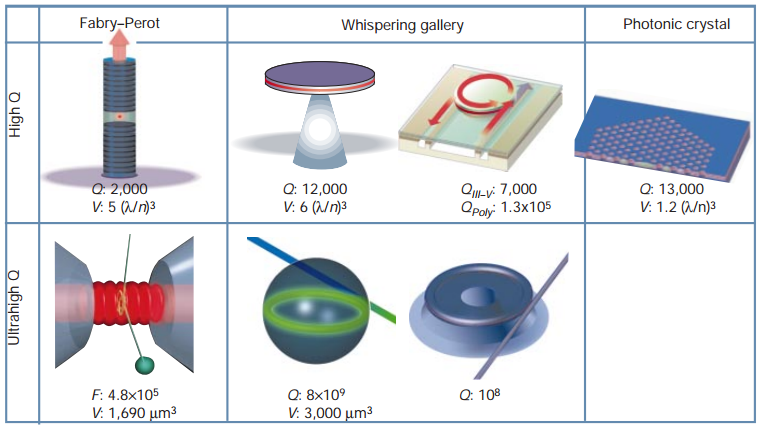
\includegraphics[width=14cm]{Microcavity}
\caption{不同种类的光学微型谐振腔,上排为高品质因子微腔,下排为超高品质因子微腔,左边一列为法布里珀罗腔,中间为回音壁微腔,右侧为光子晶体微腔。图引自\cite{vahala2003optical}}
\label{pic:Microcavity}
\end{figure}

微型谐振腔是一种能够将电磁场或光场局域在一个很小的范围内的结构。在空间上,这种结构的模式体积非常小。而在时间上,微型谐振腔非常高的光学品质因子(Q)能够保证腔中的光子泄露出腔的速率非常慢。结合了小的模式体积和很高的品质因子,微型谐振腔能够显著地增强腔中光场的能量,比自由空间中的光强增加了几个数量级。因此,当输入光功率仅仅只有1mW时,腔中的能量密度可以高达1GW/cm$^2$\cite{vahala2003optical}。这也使得微型谐振腔成为了一种用来探究非线性光学现象的极好的平台,如图\ref{pic:Microcavity}为几种典型的光学微腔示意图。用来制作微型谐振腔的材料大多数是非线性较弱的材料,如二氧化硅、氮化硅、碱金属氟化物等,对于这些材料来说,由于微型谐振腔本身对于光强极大的增强作用,使得在正常输入光下也可以看到在极高功率下才能观察到的非线性效应。而对于用具有强非线性材料制备的微型谐振腔,如铌酸锂微腔,在这种结构中可以显著降低某些非线性过程的阈值,并有效提高产率。在过去的十几年间,各种各样的非线性现象相继在微型谐振腔中被观察到,譬如,拉曼散射和拉曼激光\cite{spillane2002ultralow, cai2000fiber, kippenberg2004ultralow},布里源散射和激光\cite{li2012characterization, li2013microwave, li2014low, loh2015dual},三次谐波产生\cite{carmon2007visible, farnesi2014optical}	和四波混频\cite{kippenberg2004kerr}。这些非线性现象不仅在物理上非常有趣,而且也有许多有价值的应用,譬如,在生物传感方面\cite{ozdemir2014highly}和光学陀螺仪\cite{li2015microresonator}。

\subsection{二次谐波产生}

二阶非线性过程在量子光学中有许多有价值的应用,比如,非经典态光的产生\cite{scully1999quantum}	和量子纠缠对的产生\cite{xu2008second}。而二次谐波产生,作为最基本的二次非线性过程,通常是研究材料二阶非线性的第一步。在二次谐波产生过程当中,两个泵浦光子湮灭并产生一个拥有两倍频率的新光子\cite{boyd2003nonlinear},在正过程当中需要满足能量和动量守恒,属于典型的参量过程,而同时满足这两个守恒,也是有效产生二次谐波的条件之一,其中动量守恒又经常被称为相位匹配过程。

	二次非线性过程在非中心对称材料当中是最显著的非线性过程,这些材料包括铌酸锂、KTP等等。为了能够利用微腔增强作用,同时应用这些材料较大的二阶非线性系数,晶态铌酸锂被打磨成为微型谐振腔,Q值接近100亿\cite{ilchenko2004nonlinear}。与此同时,为了进一步能够提高转化效率,人们采用了周期极化的方法,来实现类相位匹配。之后,人们又利用铌酸锂晶体的双折射,来实现自然相位匹配,从而使得转化效率在低输入功率下提高了两个数量级\cite{furst2010naturally}。虽然打磨的方法能够制备品质因子极高的微腔,但是这种方法与标准CMOS工艺不兼容,无法批量生产,所以人们也在研究片上铌酸锂微腔,并用它成功产生了二次谐波\cite{lin2015second}。其他的一些具有较大非线性系数的材料,如砷化镓,也被用于二次谐波产生,而这里的相位匹配则利用了砷化镓晶体本身对称性的特点\cite{kuo2014second}。
	
	而在中心对称材料当中,电偶极子的二阶非线性相应是被禁止的\cite{boyd2003nonlinear}。然而,大部分和CMOS工艺相容的高品质因子、超高品质因子微型谐振腔基本都是由中心对称材料制成,如,二氧化硅\cite{armani2003ultra, kippenberg2003fabrication}	和氮化硅\cite{levy2011harmonic}。一种利用这种微腔实现二次非线性过程的方法是在这些微腔的表面镀一层非线性分子\cite{xu2008second},比如说,晶体紫罗兰\cite{dominguez2011whispering}。为了实现相位匹配,除了调节微型谐振腔的大小来控制色散并且利用更高阶径向模式以外,镀上去的非线性分子还可以被刻蚀出图案,如,可以刻成条纹状,利用非线性强度的周期性变化实现类相位匹配\cite{dominguez2011whispering}。然而,镀分子的过程本身非常复杂,而且会使得品质因子降低一到两个数量级\cite{xu2008second},这会使得非线性过程效率降低。
	
中心对称材料的一些本征的性质也可以被用来产生二次谐波。在材料的表面或者两种材料的交界面上,原本的中心对称性被打破,进而可以引入二次非线性\cite{heinz1991second}。这种非线性过程对材料表面的性质非常敏感,譬如,粘附分子或者表面化学键的一些活动。这就使得这种二次谐波产生或二次合频过程可以作为非常有效的表面性质探测器\cite{shen1989surface, shank1983femtosecond, heinz1985study, tom1986investigation}。除了表面非线性之外,中心对称性并没有禁止电四极子和磁偶极子对于二次非线性过程的相应\cite{heinz1991second},它们也是引入二阶非线性的重要渠道之一。尽管在小电介质球集合中的二次谐波产生早在二十年前就被观察到了\cite{martorell1997scattering, maymo2006visible, shan2006experimental},但直到最近,利用中心对称材料制成的微型谐振腔中的二次谐波产生过程才首次被观察到\cite{asano2016visible}。
	
\cite{asano2016visible}中的工作仅给出了780nm附近的光谱图,没有给出泵浦光光谱,没有换算出二次谐波产生功率,对于二次谐波的来源,及二次谐波功率对泵浦功率、偏振等参数的依赖关系也没有深入地研究。本文将从理论和实验两方面对二氧化硅微腔中的二次非线性现象进行深入研究,对上述几个问题都将给出答案。作为后文讨论的基础,第\ref{sec:WGM}章将对回音壁微腔中的模式进行简介;第\ref{sec:nonlinearTheo}章将介绍二次非线性的理论,是分析后文的实验结果的基础;第\ref{sec:fab}章将简述实验设计和器件制备的过程;第\ref{sec:measurement}章分析实验结果;第\ref{sec:conclu}章对全文做出总结。

\newpage
\section{回音壁模式微腔简介}
\label{sec:WGM}

二氧化硅等材料的折射率大于空气,从二氧化硅射向空气中的光会存在全反射临界角。如果将二氧化硅做成圆环、圆球等形状,光就可以在其内壁多次反射。如果光传播到圆周某处的相位条件使得每次都能形成相干增强(即谐振),则光子可以在腔中被束缚较长时间,光强也会在微腔当中得到显著增强。由于光在腔中传播类似于声音在天坛回音壁或圣保罗大教堂耳语墙的传播,如图\ref{pic:WGM},因而这种微型谐振腔得名回音壁模式微腔。

\begin{figure}
\centering
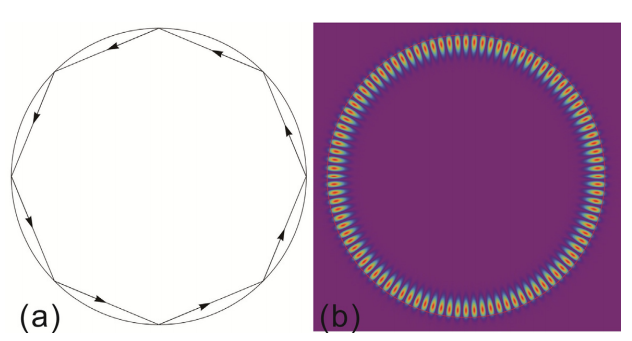
\includegraphics[width=14cm]{WGM}
\caption{回音壁模式微腔。a,声波在建筑物内壁上的反射。b,回音壁模式微腔中电场强度剖面图。图引自\cite{LiBeiBei2014}}
\label{pic:WGM}
\end{figure}

\begin{figure}
\centering
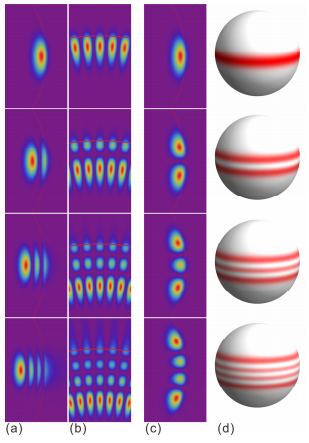
\includegraphics[scale=1 ]{mode.png}
\caption{一些不同模式数的回音壁模式的场分布。a-b, 上到下依次为$m = 50$, $q= 1\sim4$的模式在截面上和赤道面上的场分布。 c-d,从上到下依次为$q = 1$,$l = 50$,  $m = 50, 49, 48, 47$的模式在截面上和微球表面上的场分布。图引自\cite{LiBeiBei2014}}
\label{pic:mode}
\end{figure}

用光反射的射线模型描述回音壁模式的光场分布还是过于粗略,对于本次实验所采用的球腔来说,通常需要在球坐标系下解亥姆霍兹方程,解出的本征方程即为模式分布(回音壁模式求解的概述,见\cite{oraevsky2002whispering})。当掠入射条件满足时,模式与腔的外表面距离很近,此时可以近似认为电场只有球坐标系一个方向的分量,这样模式可以分为两类,电场与径向垂直(即沿角向)为TE模式;电场沿径向为TM模式。对于这两种情况,均可以将电场写成球坐标($r, \phi, \theta$)的函数并分离变量$\psi(r, \phi, \theta) = \psi_r(r)\psi_{\phi}(\phi)\psi_{\theta}(\theta)$,求解亥姆霍兹方程可得
\begin{equation}
\psi_{\phi} = \frac{1}{\sqrt{2\pi}}exp(\pm im\phi)
\end{equation}

\begin{equation}
\frac{1}{\cos(\theta)}\frac{d}{d\theta}(\cos(\theta)\frac{d}{d\theta}\psi_{\theta})-\frac{m^2}{\cos(\theta)^2}\psi_{\theta}+l(l+1)\psi_{\theta} = 0
\end{equation}
此方程的解为球谐函数$Y^l_m(\theta)$.

\begin{equation}
\frac{d^2}{dr^2}\psi_r+\frac{2}{r}\frac{d}{dr}\psi_r+(n^2k^2-\frac{l(l+1)}{r^2})\psi_r = 0
\end{equation}
其中$n$为介质折射率,$k=2\pi/\lambda$为波矢,$\lambda$为波长。此方程的解为球Bessel函数$j_r(nkr)$(腔内)和球第二类Hankel函数$h_r(kr)$(腔外)。一个球腔模式可以由四个参数确定下来,分别是角向量子数$l$,环向量子数$m$,径向量子数$q$和偏振$p$。$m$代表有$m$个环向电场强度极大值,$q$代表着径向有$q$个电场强度极大值,而角向电场强度极大值的个数由$l-m+1$来决定,一些量子数下的模式分布举例见图\ref{pic:mode}。$l, m$还满足$-l\le m\le l$。


\newpage
\section{二次非线性理论基础}
\label{sec:nonlinearTheo}
\subsection{基于电偶极子的二次非线性}
\label{sec:dipole}
在经典光学中,介质与电磁波的相互作用通常用介质极化率来描述,这一介质极化率随电场变化的函数关系可以展开为电场的幂级数,
\begin{equation}
P(t) = \epsilon_0(\chi^{(1)}E(t)+\chi^{(2)}E^2(t)+\chi^{(3)}E^3(t)+\dots)
\end{equation}
线性项被归入介质折射率中,而一阶以上的项就进入了非线性光学的范畴。非线性极化率又可以作为波动方程中的源激发出新的辐射场。
\begin{equation}
\nabla^2E-\frac{n^2}{c^2}\frac{\partial^2E}{\partial t^2} = \frac{1}{\epsilon_0c^2}\frac{\partial^2P^{NL}}{\partial t^2}
\label{eq:wave}
\end{equation}
不同阶数的非线性项将引出不同的非线性过程,这里我们主要着眼于二阶非线性项,即与$\chi^{(2)}$有关的项。

首先考虑单一频率的光输入,
\begin{equation}
E(t) = E_0e^{-i\omega t}+\textrm{c.c.} 
\end{equation}
	其中c.c.表示复共轭。这样的输入在具有二次非线性的材料当中将激发出如下的极化率
\begin{equation}
P^{(2)}(t) = 2\epsilon_0\chi^{(2)}E_0E_0^*+(\epsilon_0\chi^{(2)}E_0^2e^{-2i\omega t}+\textrm{c.c.})
\end{equation}
可以看到第一项对应着一个直流分量,不激发辐射场,被称作光学整流效应optical rectification。而第二项就产生了新的频率分量,从量子光学的角度来看,可以看成是材料中的原子吸收了两个光子,又产生了一个能量等于两个光子之和的二倍频光子,如图\ref{pic:energyLevel}(a)。

\begin{figure}
\centering
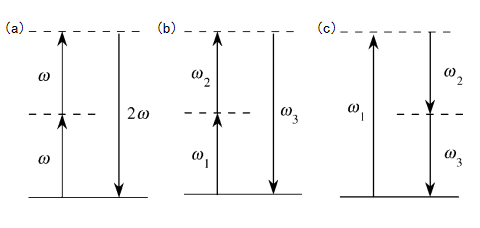
\includegraphics[scale=0.8 ]{energyLevel.png}
\caption{二次非线性过程的能级示意图。(a)二次谐波产生。(b)二次合频信号产生。(c)二次差频信号产生。图引自\cite{boyd2003nonlinear}}
\label{pic:energyLevel}
\end{figure}

当我们考虑输入光由两种频率组成,则可以通过二阶非线性产生合频和差频效应。电场可以写成
\begin{equation}
E(t) = E_1(t)e^{-i\omega_1 t}+E_2(t)e^{-i\omega_2 t}+\textrm{c.c.}
\end{equation}
该电场通过具有二次非线性的材料之后,将产生具有若干不同频率分量的极化率$P^{(2)}(t) = \sum_n P(\omega_n)e^{-i\omega_nt}$,包括
\begin{gather}
P(2\omega_1) = \epsilon_0\chi^{(2)}E_1^2 \ \ \textrm{(SHG)} \notag \\
P(2\omega_2) = \epsilon_0\chi^{(2)}E_2^2\ \  \textrm{(SHG)} \notag \\
P(\omega_1+\omega_2) = \epsilon_0\chi^{(2)}E_1E_2\ \  \textrm{(SFG)}  \\
P(\omega_1-\omega_2) = \epsilon_0\chi^{(2)}E_1E_2^*\ \  \textrm{(DFG)} \notag \\
P(0) = \epsilon_0\chi^{(2)}(E_1E_1^*+E_2E_2^*)\ \  \textrm{(OR)} \notag 
\end{gather}
其中SHG代表二次谐波产生,SFG代表二次合频信号产生,可以由图\ref{pic:energyLevel}(b)的过程来表示,DFG则是差频信号产生,可以由图\ref{pic:energyLevel}(c)的过程来表示。

介质的介电常数$\epsilon_0\chi$和材料的性质紧密相关,在经典理论当中,可以将材料中的原子(原子核+电子)看成是一个谐振子,标准的抛物线型谐振子势会带来材料的线性响应,而偏离抛物线型的谐振子势则是非线性响应的源头。

在非标准抛物线势中,又可以分为两种,一种是具有中心对称性的势,另一种是不具有中心对称性的势,一维的情况如图\ref{pic:potential}所示。电子的运动方程可以写成
\begin{equation}
\ddot{x}+2\gamma\dot{x}+\omega_0^2x+ax^2+bx^3 = -eE(t)/m
\end{equation}
其中左边第二项是阻尼项,后面的三项是谐振子势带来的加速度,右边是外加电场对于电子的影响。由此方程,结合微扰法,可以推出使用这种模型近似下的$\chi$与谐振子势的非线性系数$a$, $b$的关系\cite{boyd2003nonlinear}。其中,二次非线性系数$\chi^{(2)}$与谐振子的非对称势系数$a$成正比,即,如果材料具有中心对称性($a=0$),或材料是非晶态的(各个方向的非对称响应抵消),则$\chi^{(2)}=0$。

也可以从更高的层面上理解这个结论,对于二次谐波对应的极化率
\begin{equation}
P(t) = \epsilon_0\chi^{(2)}E^2(t),
\end{equation}
如果将电场反向,即上式中的$E(t)$变为$-E(t)$,由式子本身来看极化率不变,而根据中心对称性或非晶态材料性质,电场反向的时候,极化率也应当反向。由此推出在这类材料当中的二阶非线性极化率始终为0.

\begin{figure}
\centering
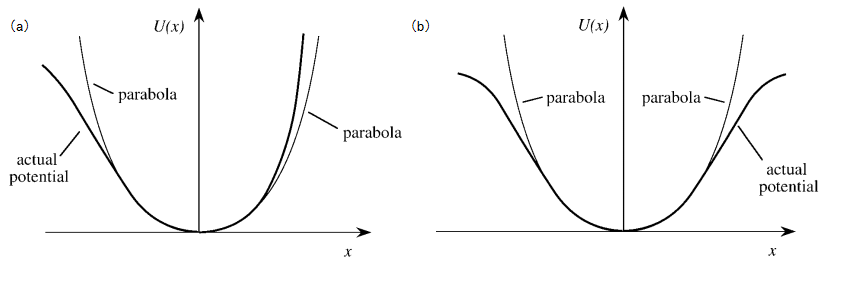
\includegraphics[scale=0.6 ]{potential.png}
\caption{原子的一维非标准抛物线势。(a)非中心对称势。(b)中心对称势。图引自\cite{boyd2003nonlinear}}
\label{pic:potential}
\end{figure}

从\ref{pic:response}中可以更加直观地看到,中心对称材料或非晶态材料的极化率随电场的变化虽然比起标准正弦形式有所变形,但依然是奇函数,不含偶次分量,即没有二次非线性响应,而非中心对称材料则会呈现出含偶次分量的特点。

\begin{figure}
\centering
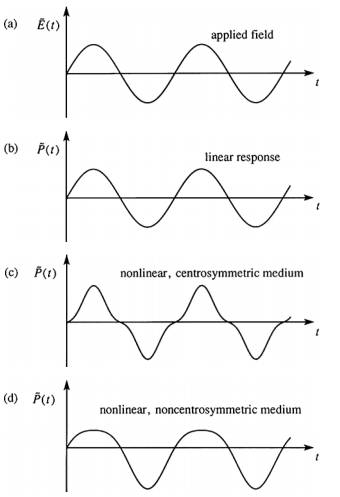
\includegraphics[scale=1 ]{response.png}
\caption{不同材料的极化率响应。图引自\cite{boyd2003nonlinear}}
\label{pic:response}
\end{figure}

\subsection{在介质表面或界面处的二次非线性}
虽然中心对称或非晶态材料的体内缺乏偶极近似下的二次非线性,在介质表面处,这种对称性被破坏,例如,最外层的原子向介质两侧振动所感受到的势是不一致的,这就会导致二次非线性的产生,同时,从直观上来看,只有靠近表面的一个薄层内具有这种表面非线性。

这里,我们在理论上探究一种最简单的情况,界面是平面,两种波长的光入射,两侧介质均为中心对称介质。将具有非线性的一个薄层抽象出一个单独的介电常数,并使其厚度趋近于0。原理图如图\ref{pic:surface},这里考虑两束光($\omega_1$, $\omega_2$)以不同的入射角射在材料界面出同一位置,反射波和投射波中都带有了新的频率分量。考虑非线性极化率的麦克斯韦方程组为
\begin{gather}
\nabla \cdot \mathbf{D}  = -\nabla \cdot \mathbf{P^{nls}} , \\
\nabla \times \mathbf{E }	+ \frac{\partial\mathbf{B} }{\partial t} = 0, \\
\nabla \cdot \mathbf{B} = 0, \\
\nabla \times \mathbf{H} - \frac{\partial \mathbf{D}}{\partial t} = \frac{\partial \mathbf{P^{nls}}}{\partial t}.
\end{gather}
由这一组方程组,结合界面两侧的边界条件,可以推出\cite{heinz1991second}
\begin{gather}
\Delta D_z = -\nabla_t \cdot \mathbf{P_s^{nls}}, \\
\Delta E_t = -1/\epsilon' \nabla_t P_{s,z}^{nls}, \\
\Delta B_z = 0, \\
\Delta \mathbf{H_t} = \partial \mathbf{P_s^{nls}}/\partial t \times \mathbf{\hat z} 
\end{gather}
其中$\Delta X = X(0^+)-X(0^-)$, $\mathbf{P^{nls}}  = \mathbf{P_s^{nls}}\delta(z)$,$\epsilon'$是界面层中的介电常数。通过上述表达式,借助菲涅耳修正,可以最终推出由这一层非线性极化层带来的向两种介质中辐射的电场信息\cite{heinz1991second}。
\begin{figure}
\centering
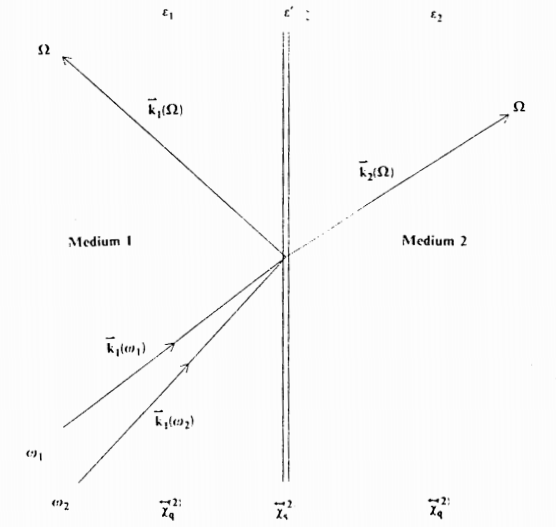
\includegraphics[scale=1 ]{surface.png}
\caption{界面二次非线性示意图。图引自\cite{heinz1991second}}
\label{pic:surface}
\end{figure}

在微型谐振腔中,依然可以通过考虑表面的非线性极化层来解决问题。具体有两种方式,一种将极化层看成厚度无限小的薄层,另一种则直接将极化层处理为空间上的$\delta$函数。首先来看第一种方法,设基波、二次谐波的电场为
\begin{equation}
\mathbf{E}_i(x,y,z,t) = a_i(t)\mathbf{E}_{0i} (x,y,z)e^{-i\omega_it},
\end{equation}
其中$i = 1, 2$分别代表基波和二次谐波,$\mathbf{E}_{0i} (x,y,z)$是空间腔膜分布,$a_i(t)$是慢变电场幅值,$\omega_i$是光场频率。由式\ref{eq:wave},得
\begin{equation}
a_2(t)\nabla^2\mathbf{E}_{02}e^{-i\omega_2t}-\frac{n^2}{c^2}\frac{\partial^2a_2(t)e^{-i\omega_2t}}{\partial t^2}\mathbf{E}_{02} = \frac{1}{\epsilon_0c^2}\frac{\partial^2\mathbf{P}^{NL}}{\partial t^2},
\end{equation}
其中
\begin{equation}
\mathbf{P}^{NL} = a_1^2(t)e^{-2i\omega_1t}\chi^{(2)}:\mathbf{E}_{01}\mathbf{E}_{01}
\end{equation}
由于$d^2 a_2/d t^2 << -i\omega_2\cdot d a_2/d t $,只保留后一项,同时注意到由于$\mathbf{E}_{02}$是腔膜的空间分布,在线性情况下满足普通波动方程
\begin{equation}
\nabla^2\mathbf{E}_{02}e^{-i\omega_2t}-\frac{n^2}{c^2}\frac{\partial^2e^{-i\omega_2t}}{\partial t^2}\mathbf{E}_{02} = 0 
\end{equation}
故由二阶非线性极化层带来的二次谐波幅度增速为
\begin{equation}
\frac{da_2}{dt} = g_sa_1^2e^{-i(2\omega_1-\omega_2)t},
\end{equation}
其中
\begin{equation}
g_s = 2i\frac{\omega_1^2}{\omega_2n^2}\frac{\int \mathbf{E}_{02}^*:\chi^{(2)}_s:\mathbf{E}_{01}\mathbf{E}_{01} d\mathbf{V}}{\int |\mathbf{E}_{02}|^2 d\mathbf{V}}
\end{equation}
注意$\chi^{(2)}$只在表面附近的区域内不为0,如果采用表面非线性系数,则分子上的积分化为$\int \mathbf{E}_{02}^*:\chi_s^{(2)}:\mathbf{E}_{01}\mathbf{E}_{01} d\mathbf{S}$。

考虑实际的腔膜还有耗散,输入输出,失谐等关系,可以得出基波、二次谐波腔膜幅度的耦合模方程\cite{haus1991coupled}
\begin{gather}
\label{eq:cpmode}
\frac{da_1}{dt} = -(\frac{\kappa_{10}+\kappa_{1e}}{2} )a_1+\sqrt{\kappa_{1e}}se^{-i(\omega_s-\omega_1)t}+g_s^*a_1a_2^*e^{i(2\omega_1-\omega_2)t} \\
\frac{da_2}{dt} = -(\frac{\kappa_{20}+\kappa_{2e}}{2})a_2+g_sa_1^2e^{-i(2\omega_1-\omega_2)t}
\end{gather}
其中$\omega_i$为腔膜的频率,$s$为输入驱动,$|s|^2$是输入功率,$\omega_s$是输入光频率,$\kappa_i0, \kappa_ie$分别是内在损耗和耦合损耗,与光学品质因子$Q$之间的关系为$\kappa_i = \omega_i/Q_i$。

将表面非线性层处理为$\delta$函数的方法比较繁琐,可参看\cite{kozyreff2008whispering}。

\subsection{由体多极效应带来的二阶非线性}
在\ref{sec:dipole}中计算的二阶非线性都是在电偶极子近似下进行的,在这种情况下,中心对称或非晶态材料中不存在二阶非线性。然而,当我们考虑更高阶的效应,如电四极子和磁偶极子时,在这些材料中依然可以出现二阶非线性。

体多极效应带来的二阶非线性可以由自由能量密度来计算\cite{bloembergen1965nonlinear,shen1984principles},化简之后的体多极效应可以表示为
\begin{equation}
P^{NL}_i = \gamma\nabla_i(\mathbf{E}\cdot\mathbf{E})+(\delta-\beta-2\gamma)(\mathbf{E}\cdot\nabla)E_i+\beta(\nabla \cdot \mathbf{E})E_i+\zeta E_i\nabla_iE_i
\label{eq:surfaceN}
\end{equation}
其中$\gamma, \delta, \beta, \zeta$是用来描述体效应的系数。其中第三项在均匀体介质中,由于$\nabla \cdot \mathbf{E}=0$所以不存在,而在非晶态材料(如熔融二氧化硅)中,$\zeta=0$,第四项也为0。可以看到,第一项对应着一个纵波$\mathbf{P}_\gamma =  \gamma\nabla(\mathbf{E}\cdot\mathbf{E})$,即,$\nabla \times \mathbf{P}_\gamma = 0$,这样的源在均匀介质当中是不会激发出辐射场的(磁场分量始终为0),然而当这个纵波传播到介质界面处的时候,则可以耦合产生正常的电磁波,并且根据边界条件计算,无论对于怎样的场分布,这一项对二次谐波产生带来的贡献将与上一节所述的表面二次非线性不可区分\cite{sipe1987new},由这一项带来的等效表面非线性系数可以写成\cite{heinz1991second}
\begin{gather}
(\chi^{(2)}_{s,\gamma})_{\perp \parallel \parallel} = \gamma_1\frac{\epsilon '(\Omega)}{\epsilon_1(\Omega)}-\gamma_2\frac{\epsilon '(\Omega)}{\epsilon_2(\Omega)}, \\
(\chi^{(2)}_{s,\gamma})_{\perp \perp \perp} = \gamma_1\frac{\epsilon '(\Omega)}{\epsilon_1(\Omega)}(\frac{\epsilon '(\omega)}{\epsilon_1(\omega)})^2-\gamma_2\frac{\epsilon '(\Omega)}{\epsilon_2(\Omega)}(\frac{\epsilon '(\omega)}{\epsilon_2(\omega)})^2
\end{gather}
其中$\epsilon ', \epsilon_1$和$\epsilon_2$分别是表面层,界面两侧的介电常数,$\Omega, \omega$分别是二次谐波和基波的频率。

在同一材料体系中,在实验上除非能够测量体内纵波的情况,否则不能通过改变光场分布来对这两种效应加以区分。另一种更具有可行性的方法则是,换用不同体和界面参数的材料进行实验,然后推知此项效应。

总而言之,式\ref{eq:surfaceN}中第一项与表面非线性无法区分,第二项是体效应,可以通过变换不同的光场分布测得材料的响应系数,第三、四项对于熔融二氧化硅来说为0.

在微型谐振腔中,第一项的贡献可以与表面非线性和在一起,写成一个等效的表面非线性系数
\begin{equation}
g_s = 2i\frac{\omega_1^2}{\omega_2n^2}\frac{\int \mathbf{E}_{02}^*:(\chi^{(2)}_s+\chi^{(2)}_{s,\gamma}):\mathbf{E}_{01}\mathbf{E}_{01} d\mathbf{S}}{\int |\mathbf{E}_{02}|^2 d\mathbf{V}}
\label{eq:gs}
\end{equation}


第二项的贡献可以写成另一个等效的基波、二次谐波耦合系数
\begin{equation}
g_b =  2i\frac{\omega_1^2}{\omega_2n^2}\frac{\int \mathbf{E}_{02}^* \cdot (\delta-\beta-2\gamma)(\mathbf{E}_{01}\cdot\nabla)\mathbf{E}_{01} d\mathbf{V}}{\int |\mathbf{E}_{02}|^2 d\mathbf{V}}
\label{eq:gb}
\end{equation}

最终的耦合模方程可以写为
\begin{gather}
\label{eq:cpmode}
\frac{da_1}{dt} = -(\frac{\kappa_{10}+\kappa_{1e}}{2})a_1+\sqrt{\kappa_{1e}}se^{-i(\omega_s-\omega_1)t}+(g_s+g_b)^*a_1a_2^*e^{i(2\omega_1-\omega_2)t} \\
\frac{da_2}{dt} = -(\frac{\kappa_{20}+\kappa_{2e}}{2})a_2+(g_s+g_b)a_1^2e^{-i(2\omega_1-\omega_2)t}
\label{eq:cpmode2}
\end{gather}

由于通过实验无法直接测量$g_s$中来自表面项和$\gamma$项的相对大小,通过理论估计,利用\cite{terhune1987second}中的数据计算,得$\chi^{(2)}_s/\chi^{(2)}_{s,\gamma}\approx 6.2$。$g_s$与$g_b$的比较可以利用\cite{rodriguez2008calibration}中给出的实验数据,但是具体数值大小依赖于基波模式和二次谐波模式的空间分布,以直径为62$\mu m$的球腔中基波模式为TM偏振,径向量子数$q$为1,角向$l$和方位角向量子数$m$均为171的模式(基模),二次谐波为TM偏振,径向量子数$Q$为2(出于相位匹配的考虑,见下一节),角向$L$和方位角向量子数$M$均为342的模式为例,得到$|g_b|/|g_s|\approx12.09$。

对于球腔来说,偏振方向以$\mathbf{r}\cdot\mathbf{H} = 0$为TM方向,$\mathbf{r}\cdot\mathbf{E} = 0$为TE方向。径向、角向和方位角向量子数的示意见图\ref{pic:mode}


\subsubsection{空间交叠积分及双共振条件}
\label{sec:2Resonance}
式\ref{eq:gs} \ref{eq:gb}的耦合系数表达式中均含有空间交叠积分,其中$g_s$的空间积分在球坐标系下对应着量子力学中的CG系数,即,需要$M=2m$, $0\le L \le 2l$,这时$g_s$才不为0。对于$g_b$,因为还涉及空间微分,所以还需考虑空间分布函数的奇偶性。总而言之,两模式之间是否有非线性耦合,不仅与材料是否有较大的非线性系数有关,还与空间交叠积分是否不为0有关。

将式\ref{eq:cpmode}\ref{eq:cpmode2}中的$a_1, a_2$换到旋转坐标系中来求解耦合模方程,$\tilde{a}_1 = a_1e^{i(\omega_s-\omega_1)t}$, $\tilde{a}_2 = a_2e^{i(2\omega_s-\omega_2)t}$,做这样变换后的耦合模方程可以写成
\begin{gather}
\label{eq:cpmoder}
\frac{d\tilde{a}_1}{dt} = [i(\omega_s-\omega_1)-\frac{\kappa_{20}+\kappa_{1e}}{2}]\tilde{a}_1+\sqrt{\kappa_{1e}}s+(g_s+g_b)^*\tilde{a}_1\tilde{a}_2^* \\
\frac{d\tilde{a}_2}{dt} = [i(2\omega_s-\omega_2)-\frac{\kappa_{20}+\kappa_{2e}}{2}]\tilde{a}_2+(g_s+g_b)\tilde{a}_1^2
\label{eq:cpmoder2}
\end{gather}

在稳态情况下,假设二次谐波产生对基波的幅度不产生影响(在二次非线性极弱的介质,如二氧化硅中是成立的),上面两式可推出输出的二次谐波功率和输入基波功率之间的关系
\begin{equation}
P_2 = \kappa_{2e}\frac{|g_s+g_b|^2}{(2\omega_s-\omega_2)^2+(\frac{\kappa_{20}+\kappa_{2e}}{2})^2}\frac{\kappa_{1e}P_1^2}{(\omega_s-\omega_1)^2+(\frac{\kappa_{10}+\kappa_{1e}}{2})^2}
\end{equation}
可以看到,在损耗和非线性耦合一定的情况下,输入光与腔膜之间的失谐越小,二次谐波的功率就越大。并且,我们希望输入光与基波、二次谐波同时达到共振,这需要满足$\Delta \omega = \omega_2 - 2\omega_1=0$,即双共振条件。

在晶体非线性光学当中,由于光频是连续分布的,故需要满足的是两种频率具有尽量接近的波矢$k$,即通常所说的相位匹配条件。而在微型谐振腔中,相位匹配条件由角量子数关系$M=2m$来满足,但同时,由于腔膜频率是分立的,因而还需要满足双共振条件来确保二次谐波的有效产生。

由于微型谐振腔中存在色散,包括材料色散和几何色散,色散使得腔中满足相位匹配条件的两个基模模式并不能满足双共振条件,图\ref{pic:mode}(a)就展示了在直径为60$\mu m$的二氧化硅微球腔中的二次谐波(SH)与基波(FW)的色散情况。可以看到,由于不同径向量子数的模式色散情况不一致,事实上可以选用SH与FW拥有不同径向量子数的情况来实现双共振条件。如,图中所示选取FW的q=1,SH的q=2,在角向量子数$l=166$附近可以实现较好的双共振条件。然而需要指出的是,即使使用这样的方法,也不能够保证精确的双共振。首先,由于模式的分立性(即,色散曲线上实际是一个个单独的点),虽然在$l=166$附近的曲线一定具有双共振,但这里并不一定有模式,如图\ref{pic:mode}(b)中的红色点所示,在这种条件下效率最好的模式由于双共振条件带来的功率降低也在$10^{-6}$量级,并且随着模式数的变化,效率也急剧下降。另一方面,实验中很难精确控制球腔的几何形状,比如直径或球的非理想性等等,以直径变化为例,图\ref{pic:mode}(b)中三种不同的直径相差极小,但是对双共振条件带来的效率影响极大,在同一波长范围内,直径稍微变动就会使得效率急剧下降。

\begin{figure}
\centering
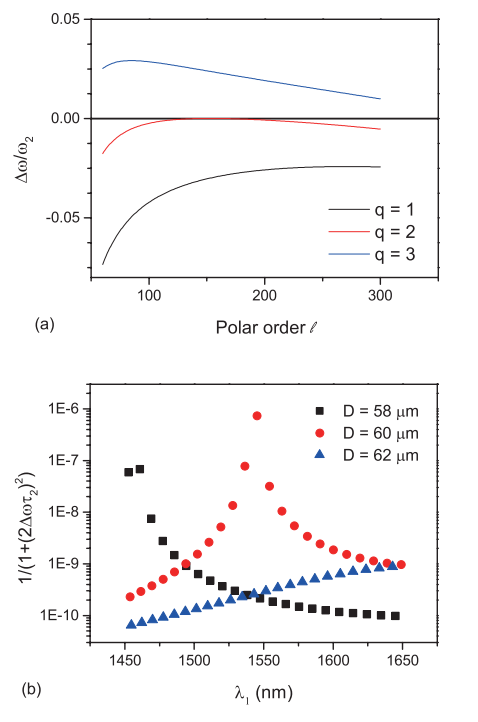
\includegraphics[width=11cm]{disp_ed2_ai.png}
\caption{\textbf{Frequency mismatch induced by dispersion. a,}   Calculated relative
frequency mismatch between SH with different radial orders q and FW as a function of
the polar order of FW.   \textbf{b,}  The calculated off-resonance coefficient of the
q = 2 mode family in microspheres with different diameters D versus the wavelength of
FW. The symbols represent modes with different polar orders separated by a free spectra
range of around 10nm.}
\label{pic:mode}
\end{figure}

为了能在实验中观察到二次谐波,必须采取其他方法来实现双共振。在上述分析当中,没有考虑微型谐振腔的热效应和Kerr非线性。这两种效应都会使得腔膜频率随着输入光功率的变化而发生变化,从而给实现双共振条件提供了可能。

在微腔中起作用的热效应主要包括热折变和热膨胀,热折变是指材料温度发生变化后,折射率也随之发生变化;而热膨胀指的是腔的体积随着温度发生变化。这两种效应结合起来,将使得腔中模式的频率发生变化,对于二氧化硅来说,单位温度变化带来的相对腔膜波长变化为$6\times 10^{-6} K^{-1}$\cite{nikogosyan2003properties,carmon2004dynamical}。较为完整的腔中热过程模型应当理解为,腔膜处能量增加,温度升高,且此热量向腔中非腔膜处及腔外扩散\cite{ilchenko1992thermal},最终达到热平衡,在新的温度下考虑此时的腔膜频率。

而Kerr效应则来源于三阶非线性系数$\chi^{(3)}$,介质极化率除了线性分量还有一个三阶非线性分量也可以产生同样频率的电磁波,$P(\omega) = \epsilon_0(\chi^{(1)}+\chi^{(3)}E(\omega)E(\omega)^*)E(\omega)$,因此也同样会产生一个随着腔中能量变化的折射率,进而引起腔膜频率的变化。

考虑这两种效果之后,得到新的耦合模方程,同样认为二次谐波的能量远远小于基波的能量,因而忽略二次谐波带来的热效应。
\begin{gather}
\label{eq:cpmodec}
\frac{d\tilde{a}_1}{dt} = [i(\omega_s-\omega_1)+iB_{11}|\tilde{a}_1|^2-\frac{\kappa_{20}+\kappa_{1e}}{2}]\tilde{a}_1+\sqrt{\kappa_{1e}}s+(g_s+g_b)^*\tilde{a}_1\tilde{a}_2^* \\
\frac{d\tilde{a}_2}{dt} = [i(2\omega_s-\omega_2)+iB_{12}|\tilde{a}_1|^2-\frac{\kappa_{20}+\kappa_{2e}}{2}]\tilde{a}_2+(g_s+g_b)\tilde{a}_1^2
\label{eq:cpmodec2}
\end{gather}
其中,
\begin{gather}
B_{11} = \frac{\int|\mathbf{E}_{01}|^4d\mathbf{V}}{\int|\mathbf{E}_{01}|^2d\mathbf{V}}[\frac{3\chi_{Kerr}\omega_1}{n_1^2}+(\frac{\partial n}{\partial T})_{eff}\frac{\epsilon_0}{\rho C \delta_{\theta 1}}\frac{\omega_1^2}{Q_{1,abs}}], \\
B_{12} = \frac{\int|\mathbf{E}_{01}|^2|\mathbf{E}_{02}|^2d\mathbf{V}}{\int|\mathbf{E}_{02}|^2d\mathbf{V}}[\frac{6\chi_{Kerr}\omega_2}{n_2^2}+(\frac{\partial n}{\partial T})_{eff}\frac{\epsilon_0}{\rho C \delta_{\theta 2}}\frac{\omega_1\omega_2n_1^2}{n_2Q_{1,abs}}]
\end{gather}
$\chi_{Kerr}$为Kerr非线性系数,$n_i$为材料在基波和二次谐波波段的折射率,$(\partial n/\partial T)_{eff}$是同时考虑了热膨胀和热折变两种效应之后的等效折射率随温度变化关系,$\rho$是材料密度,$C$是材料比热容,$\delta_{\theta i}$是表征腔膜散热的量\cite{fomin2005nonstationary},$Q_{i,abs}$代表由材料吸收所限制的光学品质因子\cite{rokhsari2004loss},品质因子由材料吸收、辐射、散射和外界耦合等因素共同决定,其中由材料吸收所带来的损耗会转化成使得腔中温度升高的能量来源。

由以上方程可以直观的看到,由热效应和Kerr效应可能补偿失谐以及未达到的双共振条件,从而实现有效二次谐波产生,下面来分析其中的物理过程。

\begin{figure}
\centering
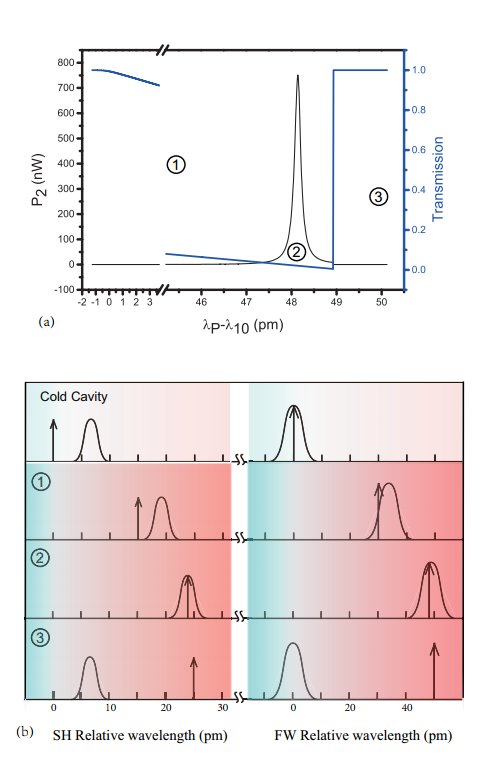
\includegraphics[width=13cm]{try_ed2}
%\caption{\textbf{Third order nonlinearity assisted double resonance. a,} The output SH power (left ordinate, black) and the FW transmission (right ordinate, blue) versus detuning in wavelength between the pump and FW. The numbers in circle indicate three different states corresponding to the schematics with the same number in panel b. \textbf{b,} Schematics of the process to achieve double resonance. The right part is the wavelength relative to the FW wavelength in cold cavity and the left part is the wavelength relative to half of the FW wavelength in cold cavity. Note that the scale of the right part is twice of that on the left. The arrows represent the pump wavelength on the right and half of the pump wavelength on the left. The Lorentz line shapes represent the FW and the SH cavity mode on the right and the left respectively. The top schematics illustrates the relative position of the pump and the cavity mode when the input power is too small to introduce obvious third order nonlinear effects while the lower ones show the position information of the corresponding states in panel a.}

\end{figure}
\begin{figure}
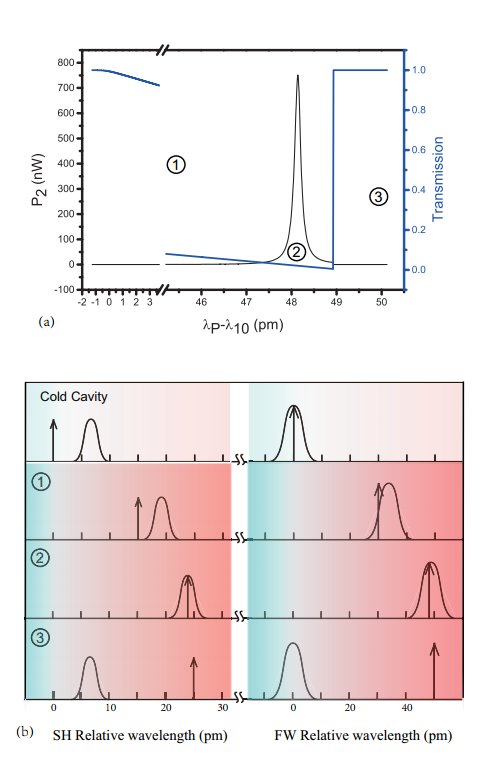
\includegraphics[width=0cm]{try_ed2}
\caption{\textbf{Third order nonlinearity assisted double resonance. a,} The output SH power (left ordinate, black) and the FW transmission (right ordinate, blue) versus detuning in wavelength between the pump and FW. The numbers in circle indicate three different states corresponding to the schematics with the same number in panel b. \textbf{b,} Schematics of the process to achieve double resonance. The right part is the wavelength relative to the FW wavelength in cold cavity and the left part is the wavelength relative to half of the FW wavelength in cold cavity. Note that the scale of the right part is twice of that on the left. The arrows represent the pump wavelength on the right and half of the pump wavelength on the left. The Lorentz line shapes represent the FW and the SH cavity mode on the right and the left respectively. The top schematics illustrates the relative position of the pump and the cavity mode when the input power is too small to introduce obvious third order nonlinear effects while the lower ones show the position information of the corresponding states in panel a.}
\label{pic:try_ed2}
\end{figure}

在二氧化硅腔中,热效应对于腔膜的影响是使腔膜产生一个红移,因而如果要增加输入功率,则腔膜红移,导致输入光和腔膜之间的失谐增大,从而由输入光到腔内能量的转化效率变低,另一方面,如果输入光功率不变,而是在蓝失谐一侧缓慢增加波长,则由于失谐逐渐减小,转化效率逐渐增加,耦合进腔的功率变大,从而使得腔膜再次红移,最终,当转化效率已经达到最大之后,输入光变到腔膜的红失谐处,导致转化效率降低,腔膜蓝移的更加厉害,最终使得输入光几乎不能耦合进腔中\cite{carmon2004dynamical}。

而如果同时考虑二次谐波腔膜的移动,如图\ref{pic:try_ed2}(b)所示,当腔中能量极小时(cold cavity),输入光与基波共振,但其二倍频不与二次谐波模式共振,此时二次谐波产生效率极低。如果输入光功率足够大,则基波和二次谐波腔膜都会发生红移,但是二次谐波腔膜的移动要比输入光的二倍频移动速度慢,则如果开始时输入光二倍频与二次谐波腔膜是蓝失谐的位置关系,则在某一失谐时,能够满足双共振条件图\ref{pic:try_ed2}(b2),此后,如果波长继续增大,则会从两个腔膜中跳出。此过程对应的二次谐波能量和基波经过腔的透射谱如图\ref{pic:try_ed2}(a)所示。

由上述过程可知,如果输入光功率较小,则即使有腔膜移动,也不足以达到双共振条件,因而产生二次谐波功率极低,当输入光功率达到某一临界值时,恰好能够达到双共振条件,当输入光功率继续增大,则在基波达到共振前二次谐波就达到了共振,此时对于实验来说最为稳定,但由于基波未达到共振,虽然输入功率增加了,总体而言产生二次谐波的功率并没有显著变化,该过程如图\ref{pic:P2change_ed2_ai}(a)所示。

转化效率随耦合系数$K$的变化如图\ref{pic:P2change_ed2_ai}(b)所示,在临界耦合的时候转化效率达到最高。不同波长对应的临界功率与色散曲线有关图\ref{pic:P2change_ed2_aicd}(c),但一般来说,转化效率与临界功率成正比,这与二次谐波的二阶功率关系是相适应的,同时可以看到,同一个临界功率下,球越大,转化效率会越低,可能是由于球大了之后场比较弥散且更靠近体内,因而表面和体的非线性效应都会有所下降,如图\ref{pic:P2change_ed2_aicd}(d)。
\begin{figure}
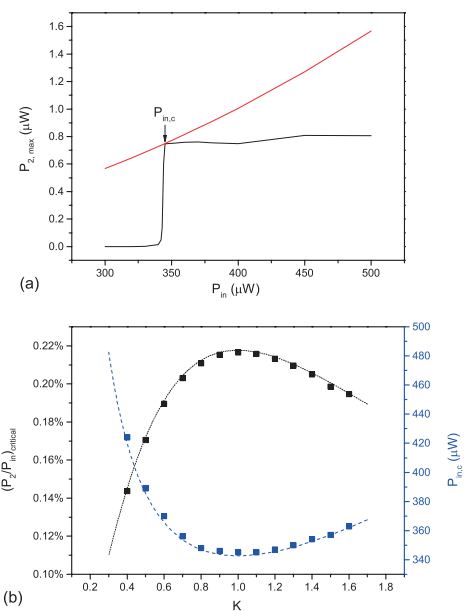
\includegraphics[width=11cm]{P2change_ed2_ai}
\centering
\caption{\textbf{Maximum output SH power and efficiency. a,} The maximum output SH power versus input power. The red line is the ideal output SH power by setting the off-resonance coefficient to one. The black line represents the maximum output SH power considering all the possible detuning (corresponds to state 2 in Fig. 2a). \textbf{b, } The conversion efficiency at the critical input power (left ordinate, black) and the critical input power (right ordinate, blue) as a function of coupling coefficient K. The dashed lines are results of the analytical expression and the symbols are calculated numerically with nonlinear coupled-mode equations. \textbf{c-d, } The influence of different diameters of microsphere and various polar order $l$. }
\label{pic:P2change_ed2_ai}
\end{figure}

\begin{figure}
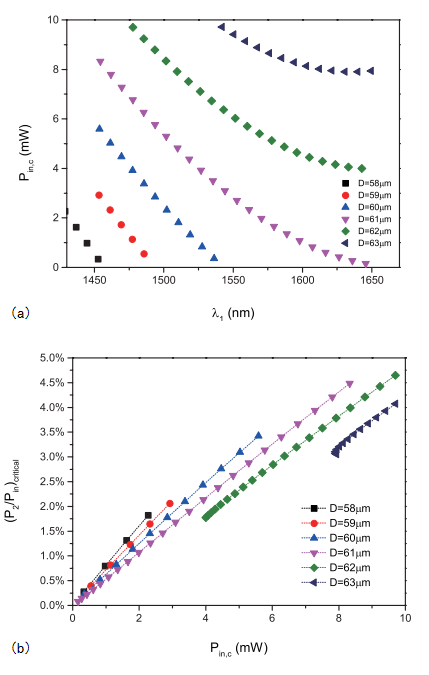
\includegraphics[width=11cm]{P2change_ed2_aicd}
\centering
\caption{\textbf{Influence of the size of microcavity. c,} The critical input power versus the FW wavelength. The symbols represents a pair of FW and SH modes with $l_2=2l_1$.  \textbf{d, }The critical conversion efficiency as a function of different critical input power. The symbols are the same with those in panel c and the dashed lines are only guides for the eye. }
\label{pic:P2change_ed2_aicd}
\end{figure}

\newpage
\section{实验设计与器件制备}
\label{sec:fab}
\subsection{实验设计}
\label{sec:ExpSetup}

从原理上考虑实验设计非常简单,只需要将泵浦光有效地耦合进腔,再通过合适的方式探测产生的二次谐波即可,不论是表面还是体多极二次非线性,都是腔内在的性质,不直接依赖于输入输出关系。\cite{carmon2007visible}中的三次谐波产生就只用了最简单的光纤锥耦合的方法,并用CCD摄像头收集产生的绿光。

对于本实验来说,由于信号光的光强非常弱,需要解决两个技术问题,一是如何有效收集二次谐波信号,二是如何有效探测二次谐波信号。如果采用\cite{carmon2007visible}中的方法,用传统CCD完成收集和探测的任务会导致实验装置复杂,且收集效率低。而如果仅用针对泵浦光的光纤锥收集,则由于泵浦光光纤锥是专门针对泵浦光设计的,仅在泵浦光波段能够达到临界耦合,在信号光波段由于无法较好地匹配光纤锥和球腔当中的波矢,收集效率非常低,另一方面,信号光在通信波段光纤中传播的过程中也会有较大的损失,这是三次谐波实验当中没有用光纤锥进行收集的主要原因。而我们认为,这也是之前实验当中几乎没有人观测到二次谐波信号的重要原因。

本实验中为了解决第一个问题,在泵浦光光纤锥之外,又专门加入了一根信号光光纤锥。在制备的时候,信号光光纤锥就设计为达到了信号光波段的单模条件,可以实现该波段的波矢与微球腔当中的波矢匹配,从而达到较高的耦合效率。而为了解决第二个问题,从信号光光纤锥中收集到的信号最终被送到EMCCD(电子放大电荷耦合器件)当中,与普通的CCD相比,EMCCD加入了电子放大功能,探测器部分也有专门的冷却装置,整体能够实现更高的信噪比,从而完成对弱信号的探测。

%如果仅使用这种实验设计,就完全与\ref{sec:2Resonance}中的理论分析一致,这将会导致二次谐波输出功率随着泵浦光功率呈一个阶跃式的变化,无法验证二次谐波功率与输入功率呈平方关系的特性。因而,在基础实验设计之上,再使用一路控制光源,专门用于调控腔的热效应及Kerr效应,使得达到双共振条件时的腔内泵浦光光强可以在较大范围内变化。

\begin{figure}
\centering
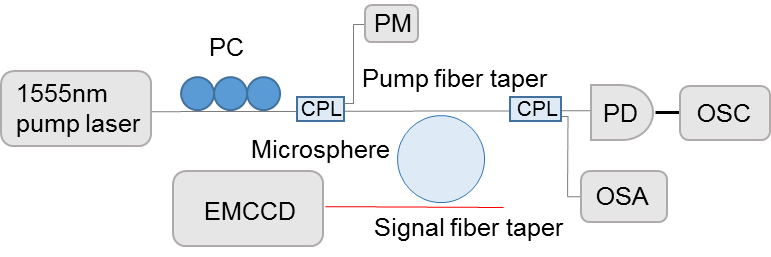
\includegraphics[width=16cm ]{ExpSetup.png}
\caption{实验设计示意图。pump laser:泵浦光激光光源;PC:偏振控制器;CPL:光耦合器;PM:光功率计;Microsphere:微球谐振腔;PD:光探测器;OSC:示波器;OSA:光谱仪;EMCCD:电子放大电荷耦合元件;Pump fiber taper:泵浦光波段相位匹配的光纤锥;Signal fiber taper:信号光波段相位匹配的光纤锥。}
\label{pic:ExpSetup}
\end{figure}

如图\ref{pic:ExpSetup}所示,泵浦光在1555nm附近,经过PC(偏振控制器)调节偏振后,输入泵浦光耦合光纤锥中。首先通过CPL分出一部分光进入OSA(光谱仪)中检测通讯波段光谱和拉曼等信号,另一部分光输入PD(光探测器)将光信号转化为电信号最后输入OSC(示波器)进行,监测泵浦光的透射谱。

二次谐波这一路光信号由二次谐波波段的光纤锥进行收集,并送入EMCCD(电子放大电荷耦合器件)中进行光谱探测。

\subsection{微球腔的制备}

%装置照片,制备步骤,成品照片,Q值,Transmission谱,半径,选取半径值的原因
\begin{figure}
\centering
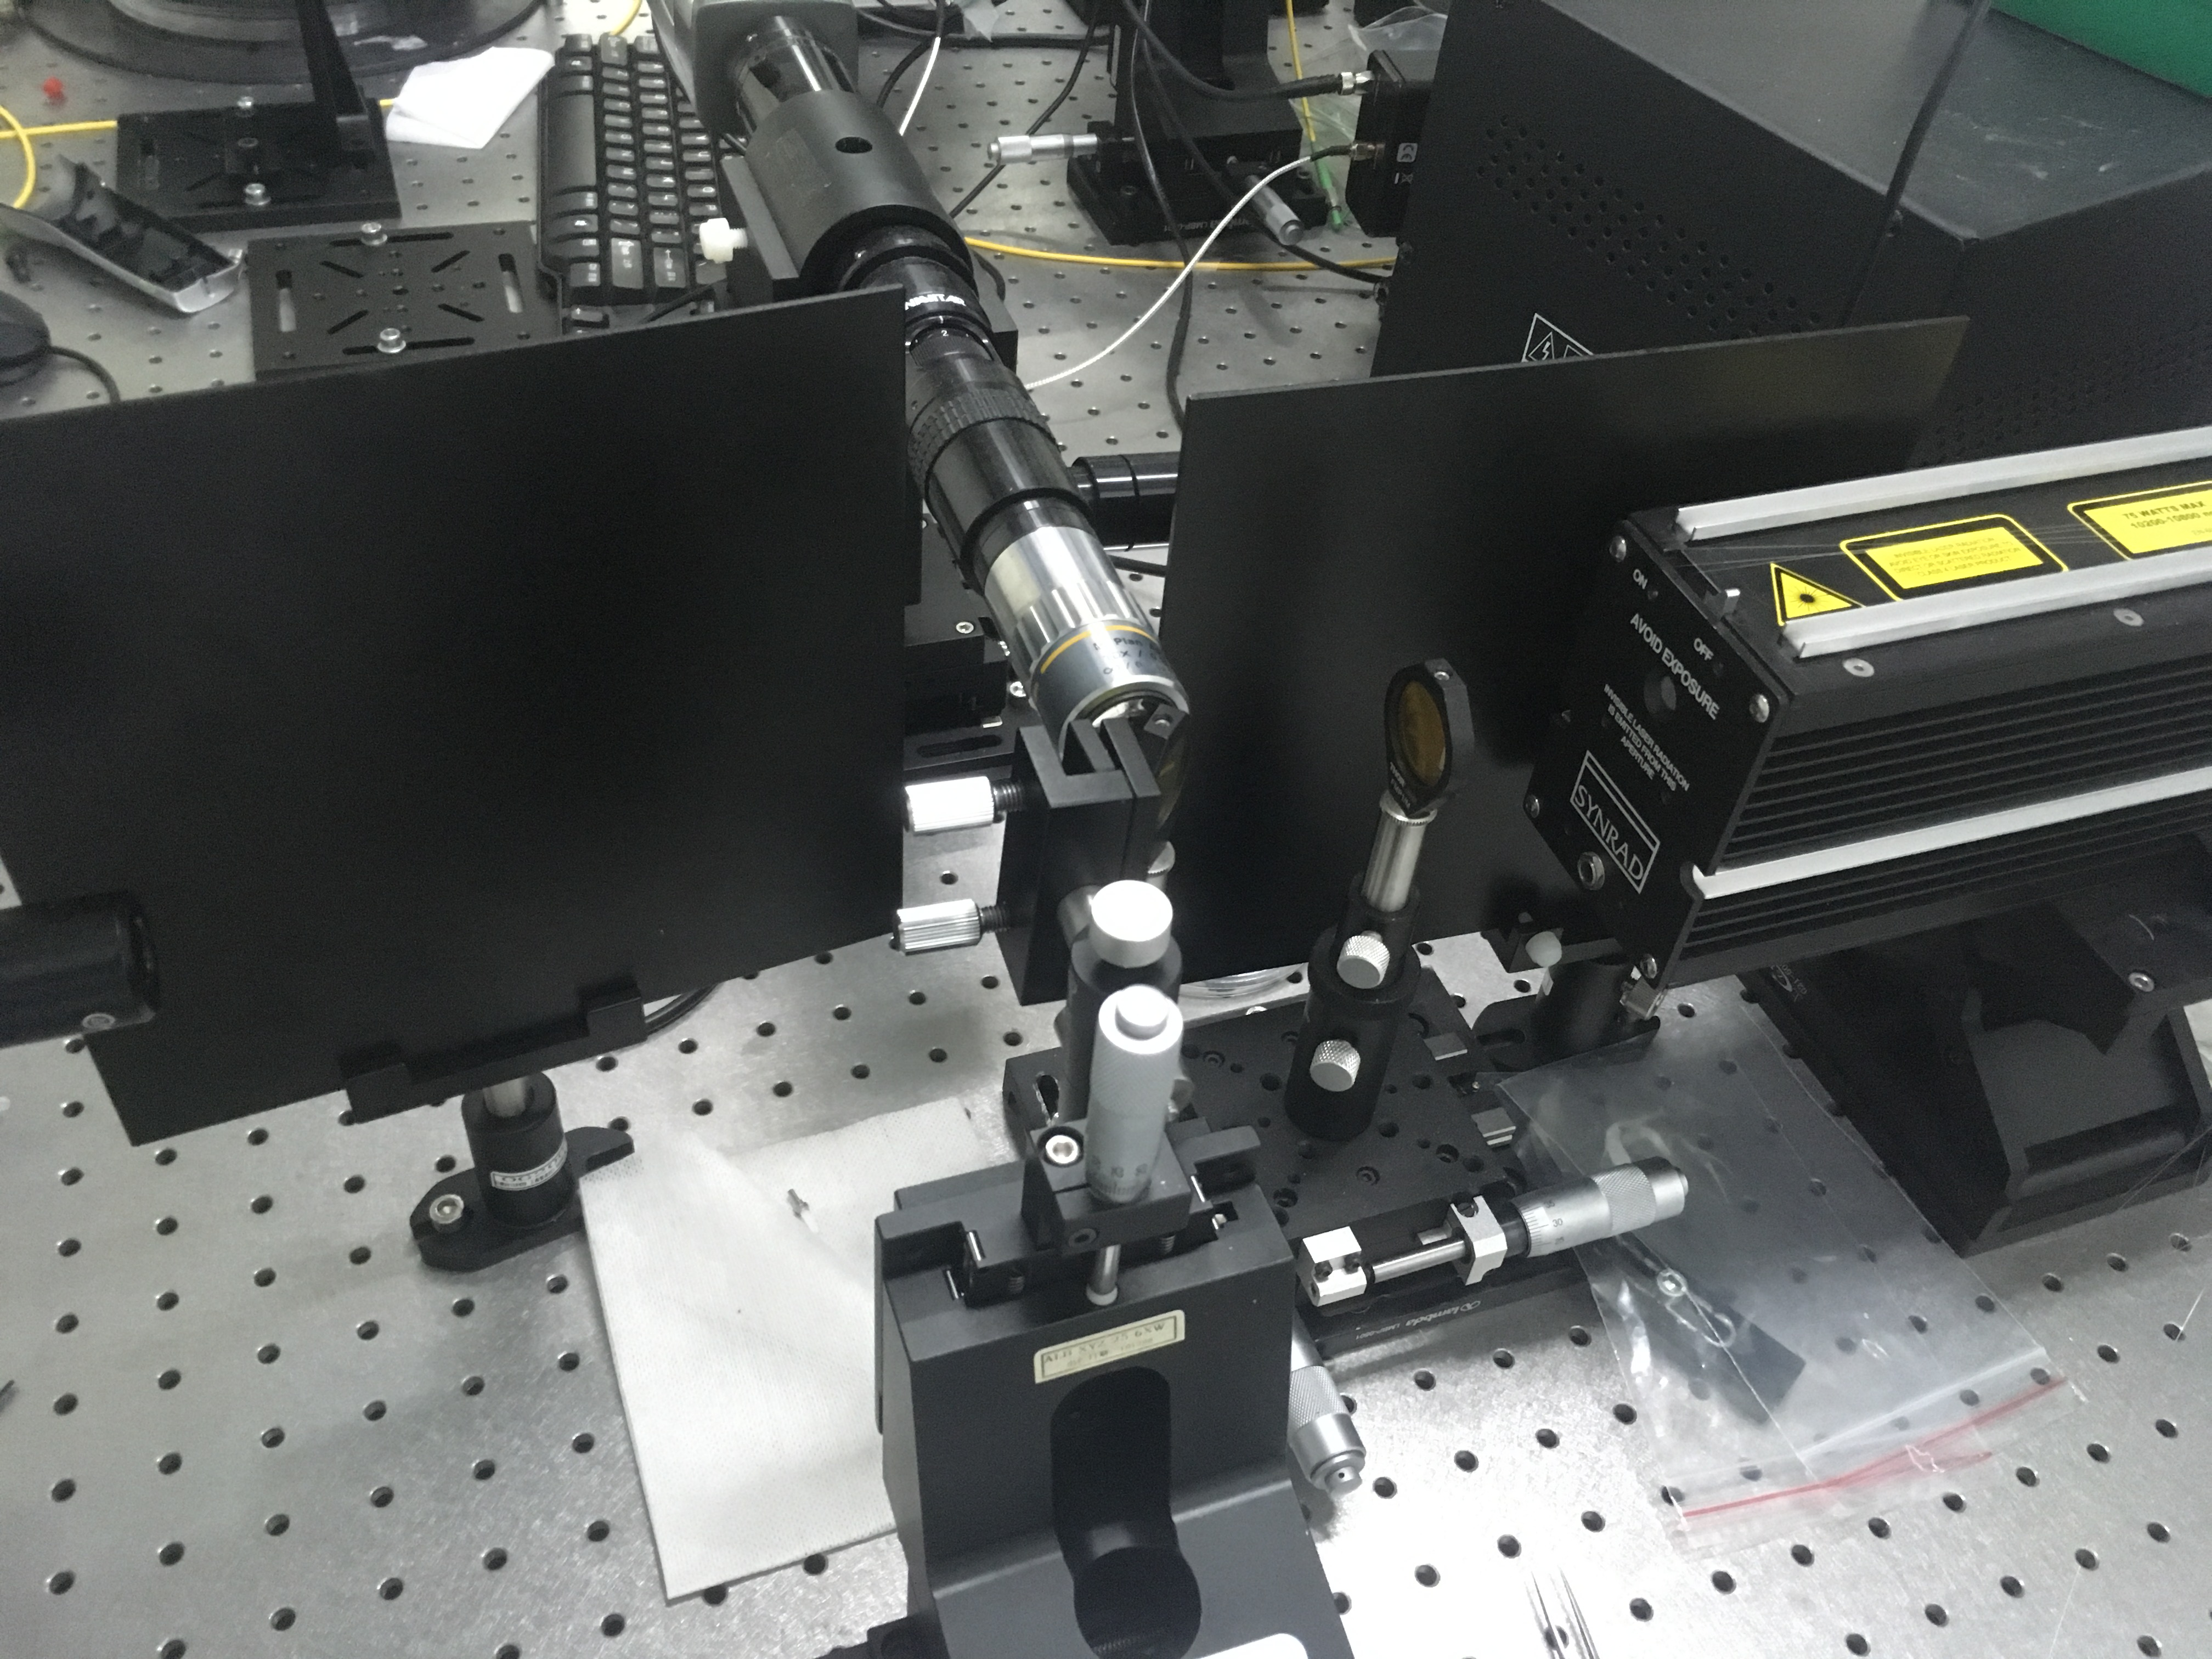
\includegraphics[width=16cm ]{Setup_makingSphere}
\caption{微球腔制备实验装置图}
\label{pic:Setup_makingSphere}
\end{figure}

微球腔的制备主要使用图\ref{pic:Setup_makingSphere}中的装置,图片右侧为一台二氧化碳激光器,输出约10$\mu m$波长的激光,主要产生热效应,激光通过前方放置的透镜聚焦。制备时首先取一小段清洁的去包层光纤,下坠一个重物(如垫片),固定在玻片上,将玻片夹持在三维平移台上,通过图中所示的成像系统进行成像,用来调整光纤的位置,使得操作点在三个维度上都与激光器输出光的焦点重合。

通过函数信号发生器产生的方波来控制二氧化碳激光器的出光,方波为最大值时激光器出光,为零时不出光,这样可以通过控制方波的占空比来控制激光器的有效出光功率。

根据有效出光功率的不同,微球腔的制备可以分为三个阶段:第一阶段,采用较小的占空比(本实验中为7.5\%)出光约0.2s,配合重物,将光纤中的一段拉细拉长而不至于断裂,可以将原直径为125$\mu m$的光纤拉细为直径$10\mu m$以下,这是为了使得一般大小的微球(如,本实验中的62$\mu m$直径微球)的根部不会对整个微球的形状产生大的影响;第二阶段,将光纤上移至细光纤底部与粗光纤交界处在焦点上,提高占空比(本实验中为20\%),可以在很短时间内将光纤打断,下端随重物落下,上端则熔成一个近似于微球状的核;第三阶段,采用较高的占空比(本实验中为17\%),聚焦在微球下方约200$\mu m$处,对微球和光纤进行加热,使得微球熔化上卷,不断消耗细光纤,微球的体积也逐渐增大,当微球上卷到细光纤部分只剩下约10$\mu m$的时候,停止加热,微球腔制备完成。

在实验中,可以通过经验性地控制第二阶段打断细光纤的位置来控制球腔的大小,但做不到非常精确。因此也没有办法通过这种方法精确控制腔的色散,所以需要用\ref{sec:2Resonance}中的方法来实现双共振。理论仿真的结果表明,在微球直径为60$\mu m$或略大一些时,能够在1550nm波段比较接近双共振条件,之后再进用三次非线性辅助的方法接近双共振条件会更容易。因此在实验中,我们尽可能地选用这样尺寸的微球,最终测得下一章中用来产生二次谐波的微球直径为62$\mu m$。


\subsection{双光纤的制备与操控}

拉光纤装置照片,步骤,成品照片,透过率,操控光纤耦合方法,耦合球腔照片

\begin{figure}
\centering
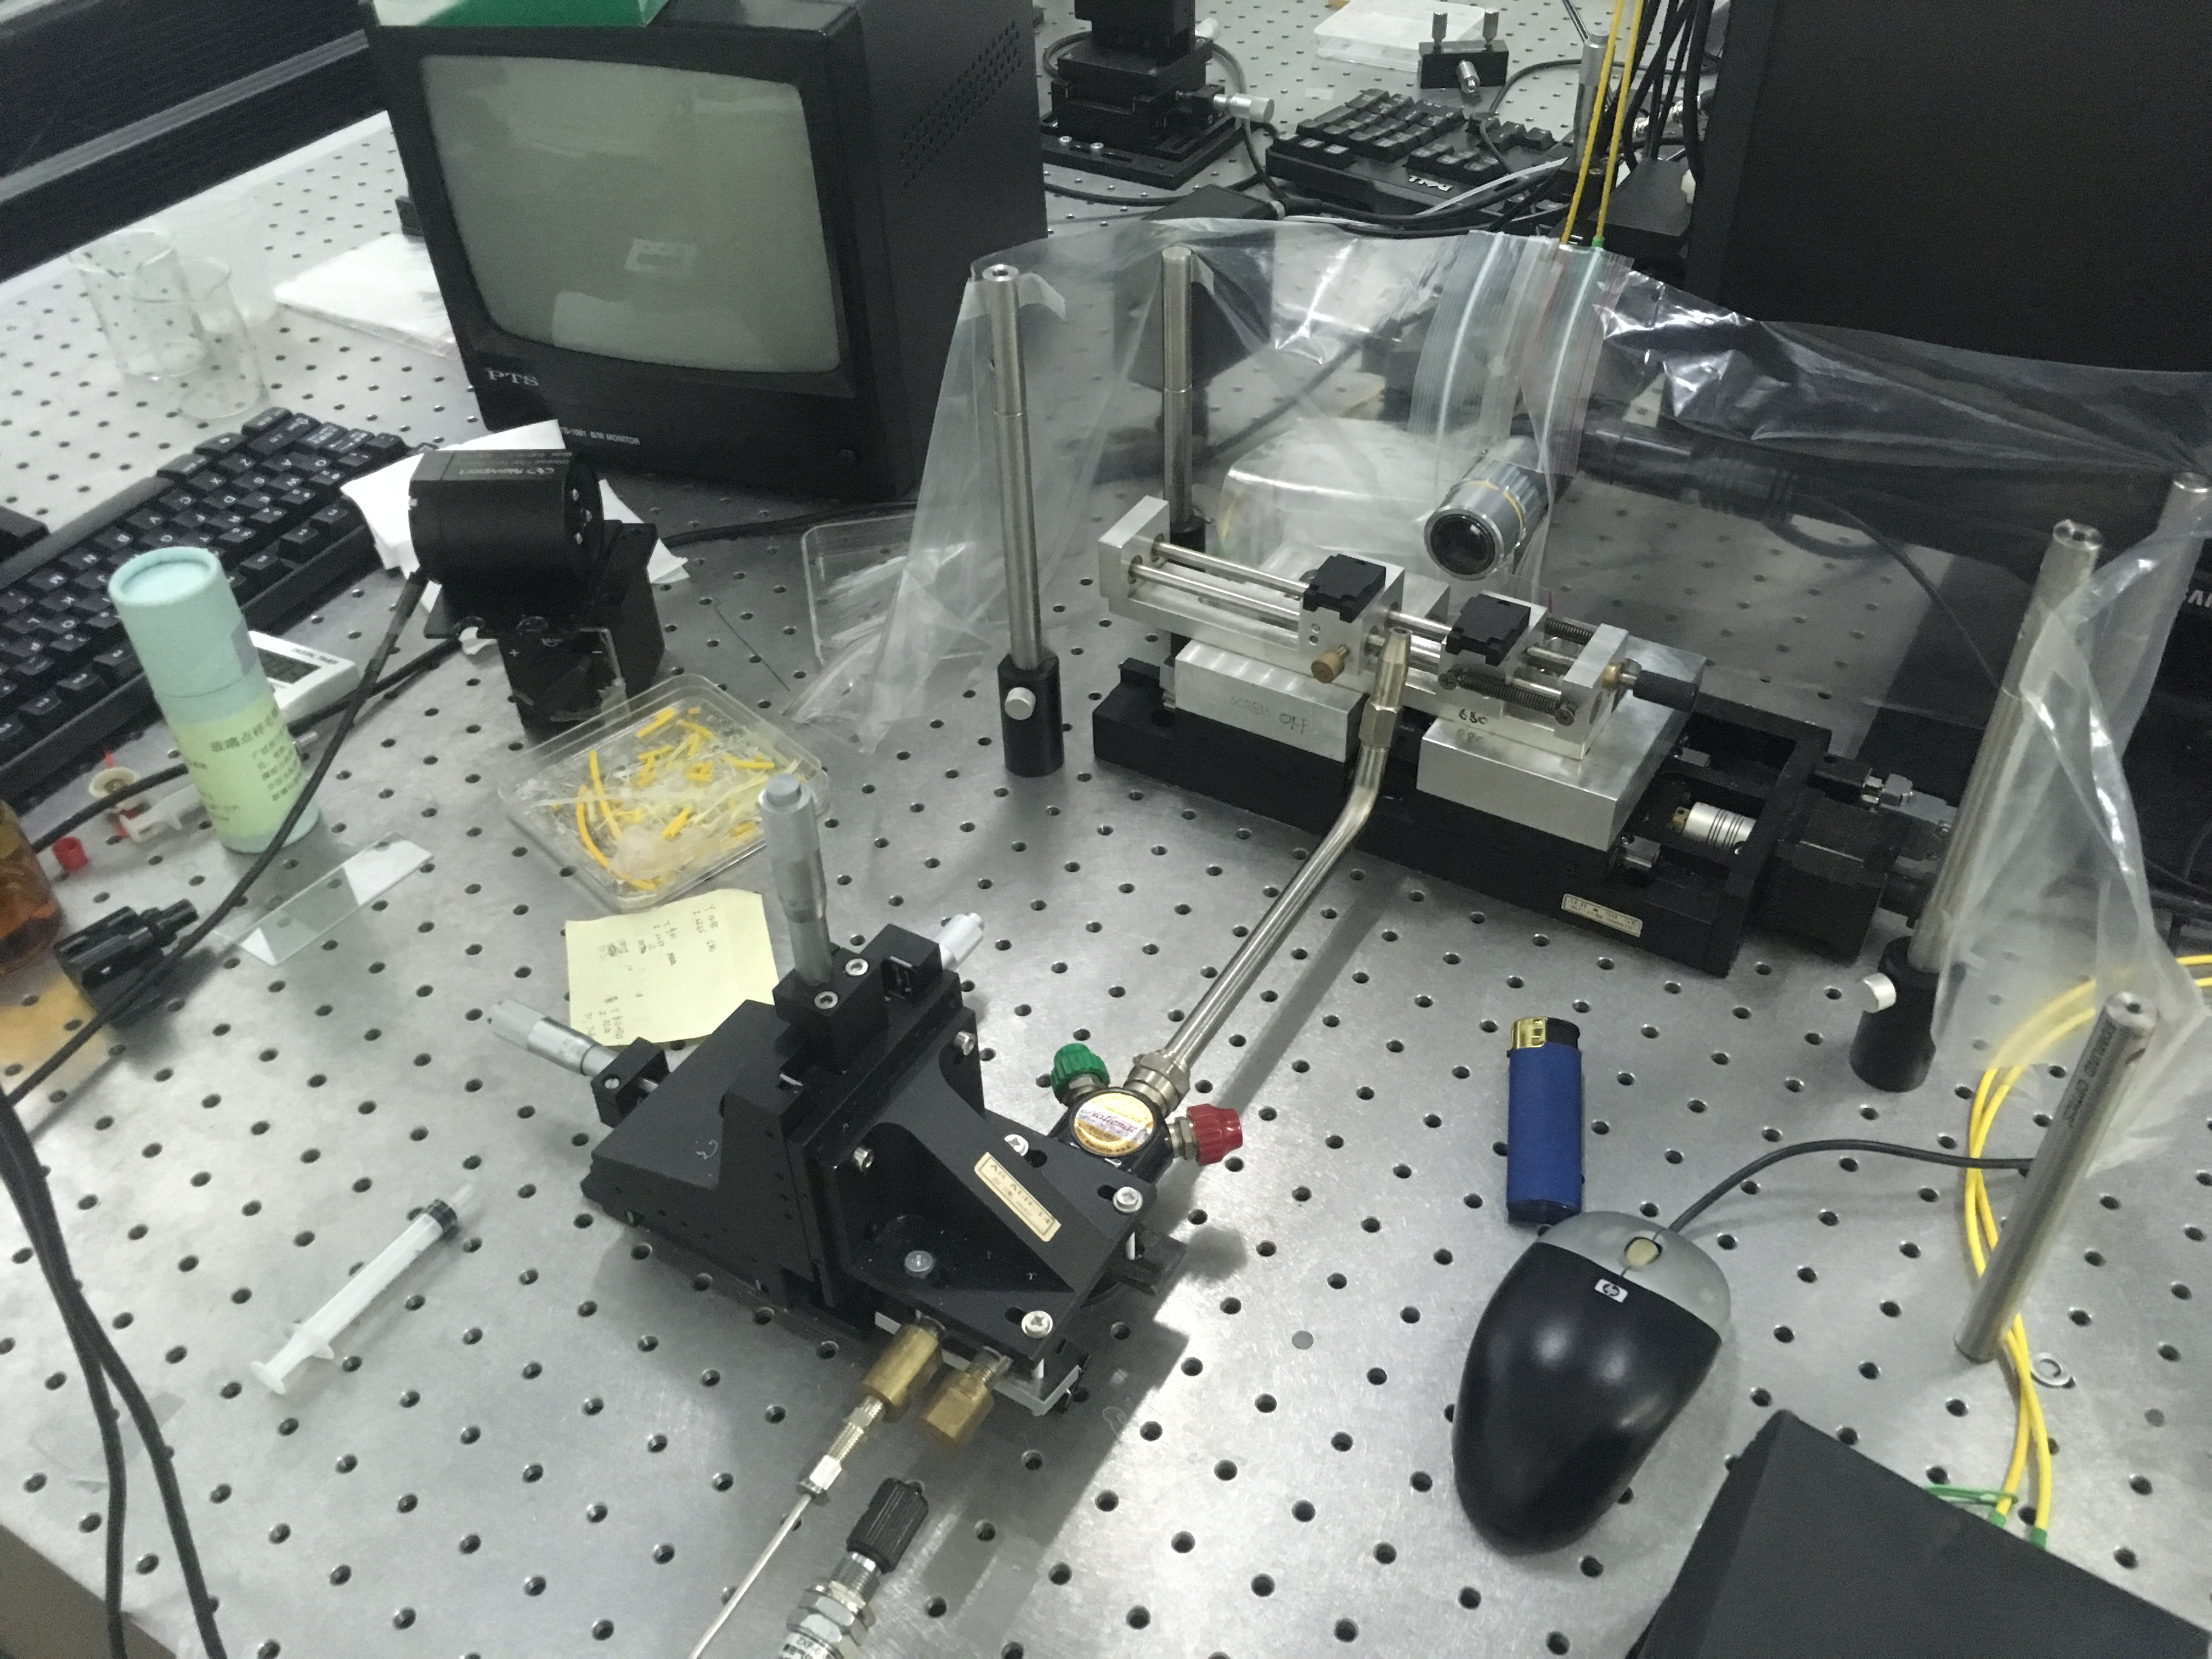
\includegraphics[width=16cm ]{Setup_pullingFiber}
\caption{双光纤制备实验装置图}
\label{pic:Setup_pullingFiber}
\end{figure}

图\ref{pic:Setup_pullingFiber}所示是用来制备双光纤的实验装置。从原理上来讲,光纤锥是通过氢氧焰对光纤中部进行加热,配合两边电机驱动将光纤拉长,使得受热部分变细,直到受热部分的直径达到该波段的单模条件,此时光纤锥中的波矢与球腔中基模的波矢相近,能够实现较好的耦合效率。

在实验上,可以通过调节火焰的位置找到一个最佳加热点,使得在达到单模条件时由于光纤变细造成的损耗较小,针对1550nm波段的光纤锥,在最优位置,损耗可以降低到1$\%$以下。而对于双光纤来说,主要有两个难点,一是使得两根光纤在各自波段能几乎同时达到单模条件,不至于使得后达到单模条件的光纤制备好时第一根光纤已经变得太细,影响耦合;另一个难点是要同时使得两根光纤的损耗尽可能小。经过反复试验,得到一组参数,可以稳定地使两根光纤同时达到单模条件。对于这组参数,泵浦光光纤锥的损耗为3$\%$,信号光光纤锥的损耗为35$\%$。

具体制备步骤如下:首先将两根光纤分别通1555nm波段和778nm波段的光,接在光探测器上随时检测功率;之后在两根光纤中部选取合适的位置各自拨开长约1cm的包层,用酒精擦拭干净,卡在最细的夹槽中,需要注意的是,最细的夹槽是为单光纤设计的,两根光纤一起放有时会在拉动过程中打滑,不利于制备,所以实验中用贴纸做固定;接下来点燃氢氧焰,对光纤中部预热3分钟;预热好后,控制电机向两侧拉光纤,同时通过光探测器检测两根光纤的输出功率,在达到单模条件之前,光纤输出功率会反复震荡,最终在达到单模条件时稳定,此时同时关闭火焰和电机;最后利用成像系统检查两根光纤是否完好,是否过于松弛影响耦合等,并进行相应调整。

\begin{figure}
\centering
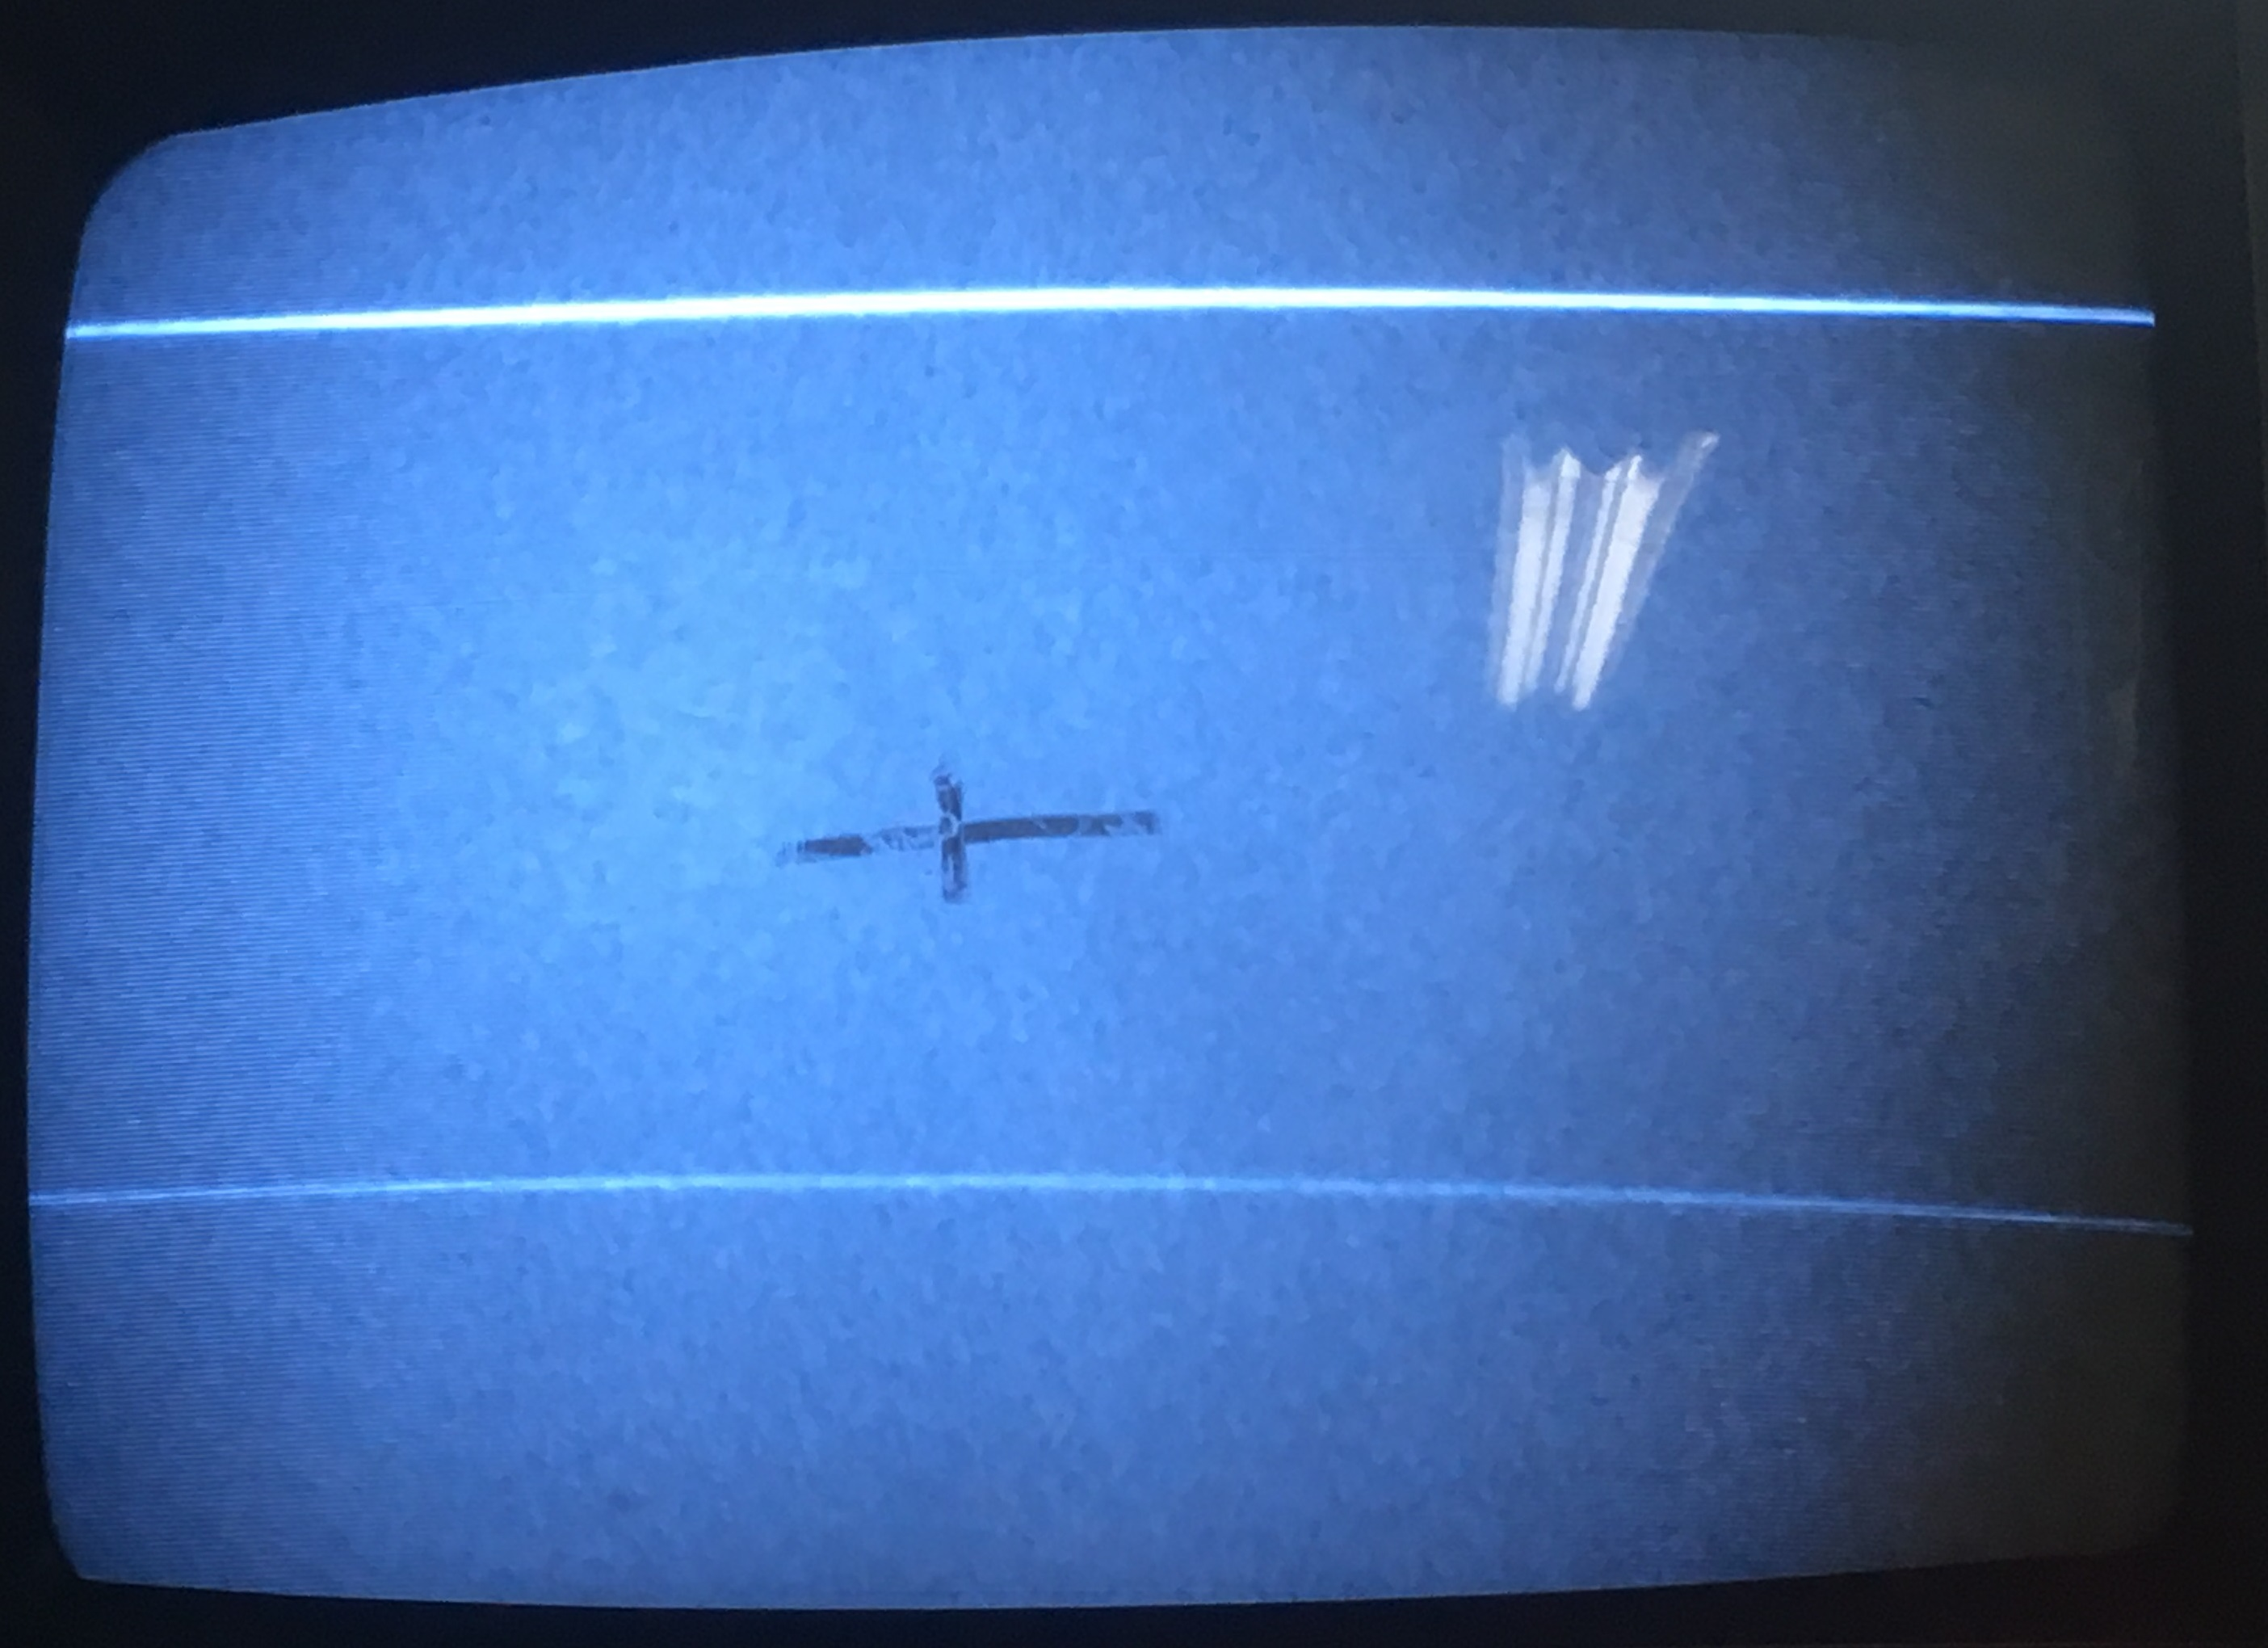
\includegraphics[width=16cm ]{DualFiber}
\caption{双光纤锥的顶视图,上面的是泵浦光光纤锥,下面是信号光光纤锥}
\label{pic:DualFiber}
\end{figure}

图\ref{pic:DualFiber}是双光纤的顶视图,上面的是泵浦光光纤锥,下面是信号光光纤锥,可以看到泵浦光光纤锥比信号光光纤锥要粗,这是由于泵浦光波长约为信号光的两倍,在达到单模条件时,光纤锥直径也会更大。

\begin{figure}
\centering
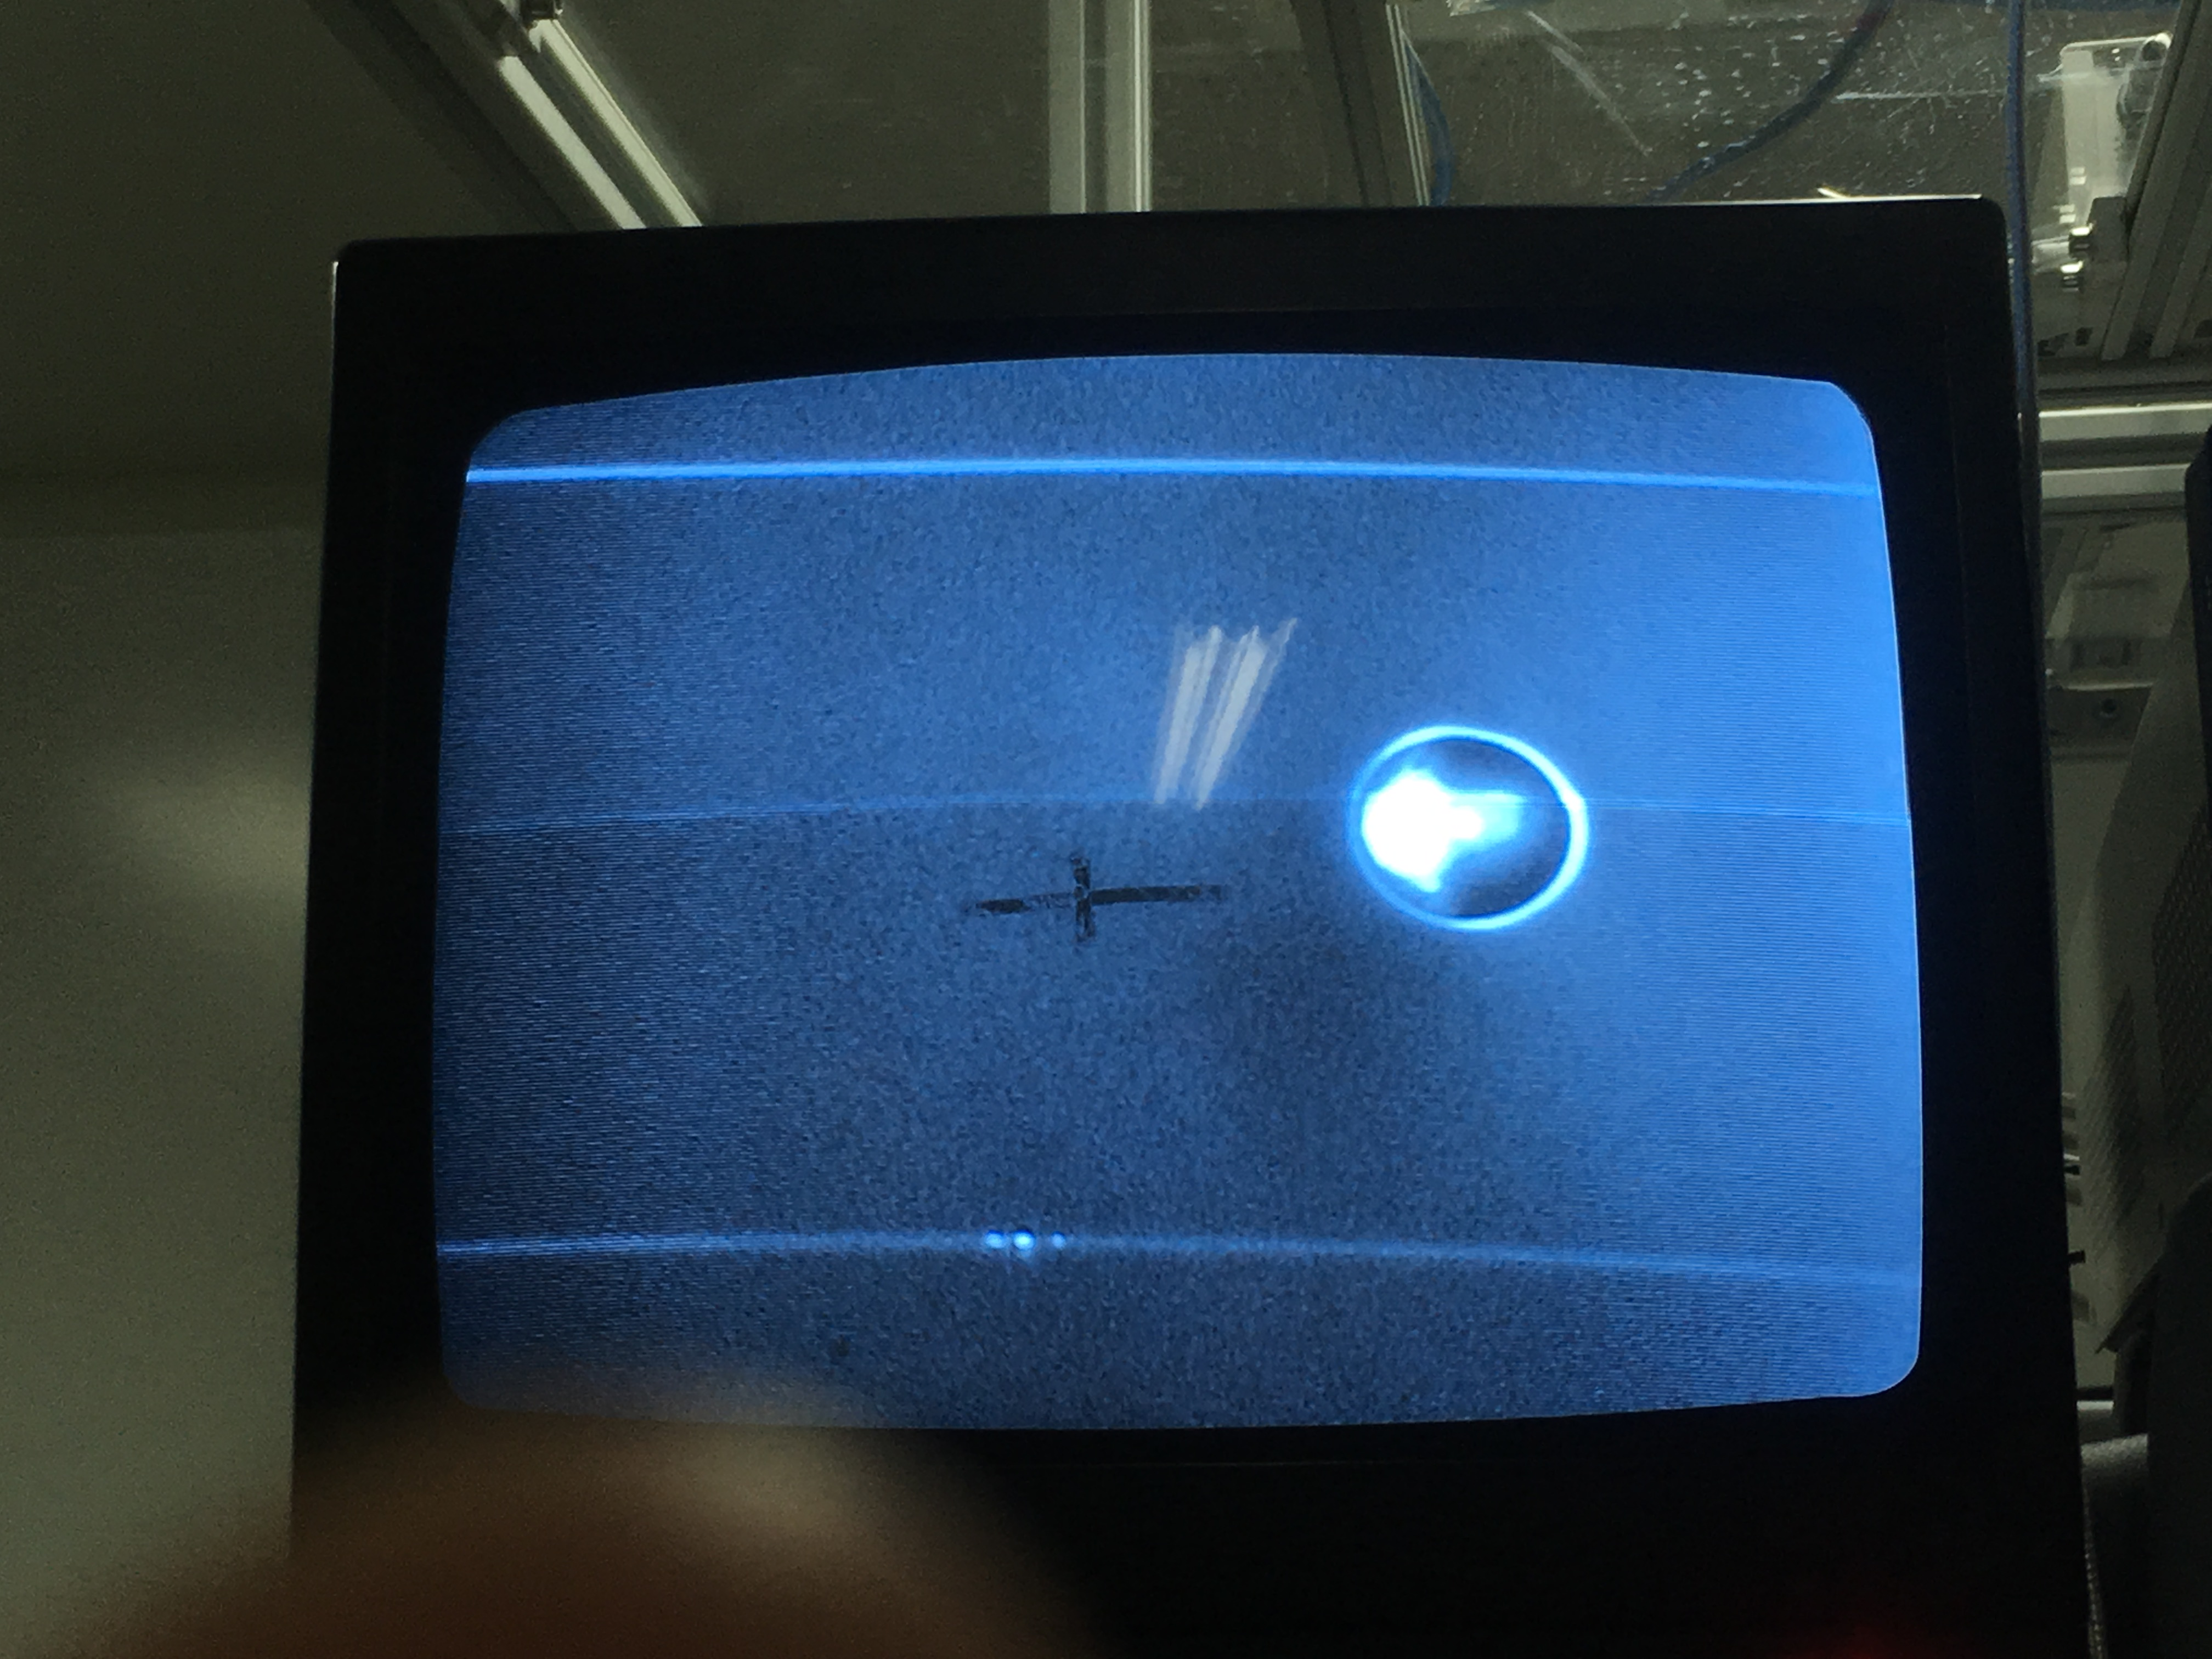
\includegraphics[width=16cm ]{Fiber_sphere}
\caption{进行耦合前的光纤锥和微球腔顶视图}
\label{pic:Fiber_sphere}
\end{figure}

图\ref{pic:Fiber_sphere}是进行耦合前的光纤锥和微球腔顶视图,微球腔的固定是将光纤杆与地面垂直地贴在垫块上,故在顶视图中看不到光纤杆。

\begin{figure}
\centering
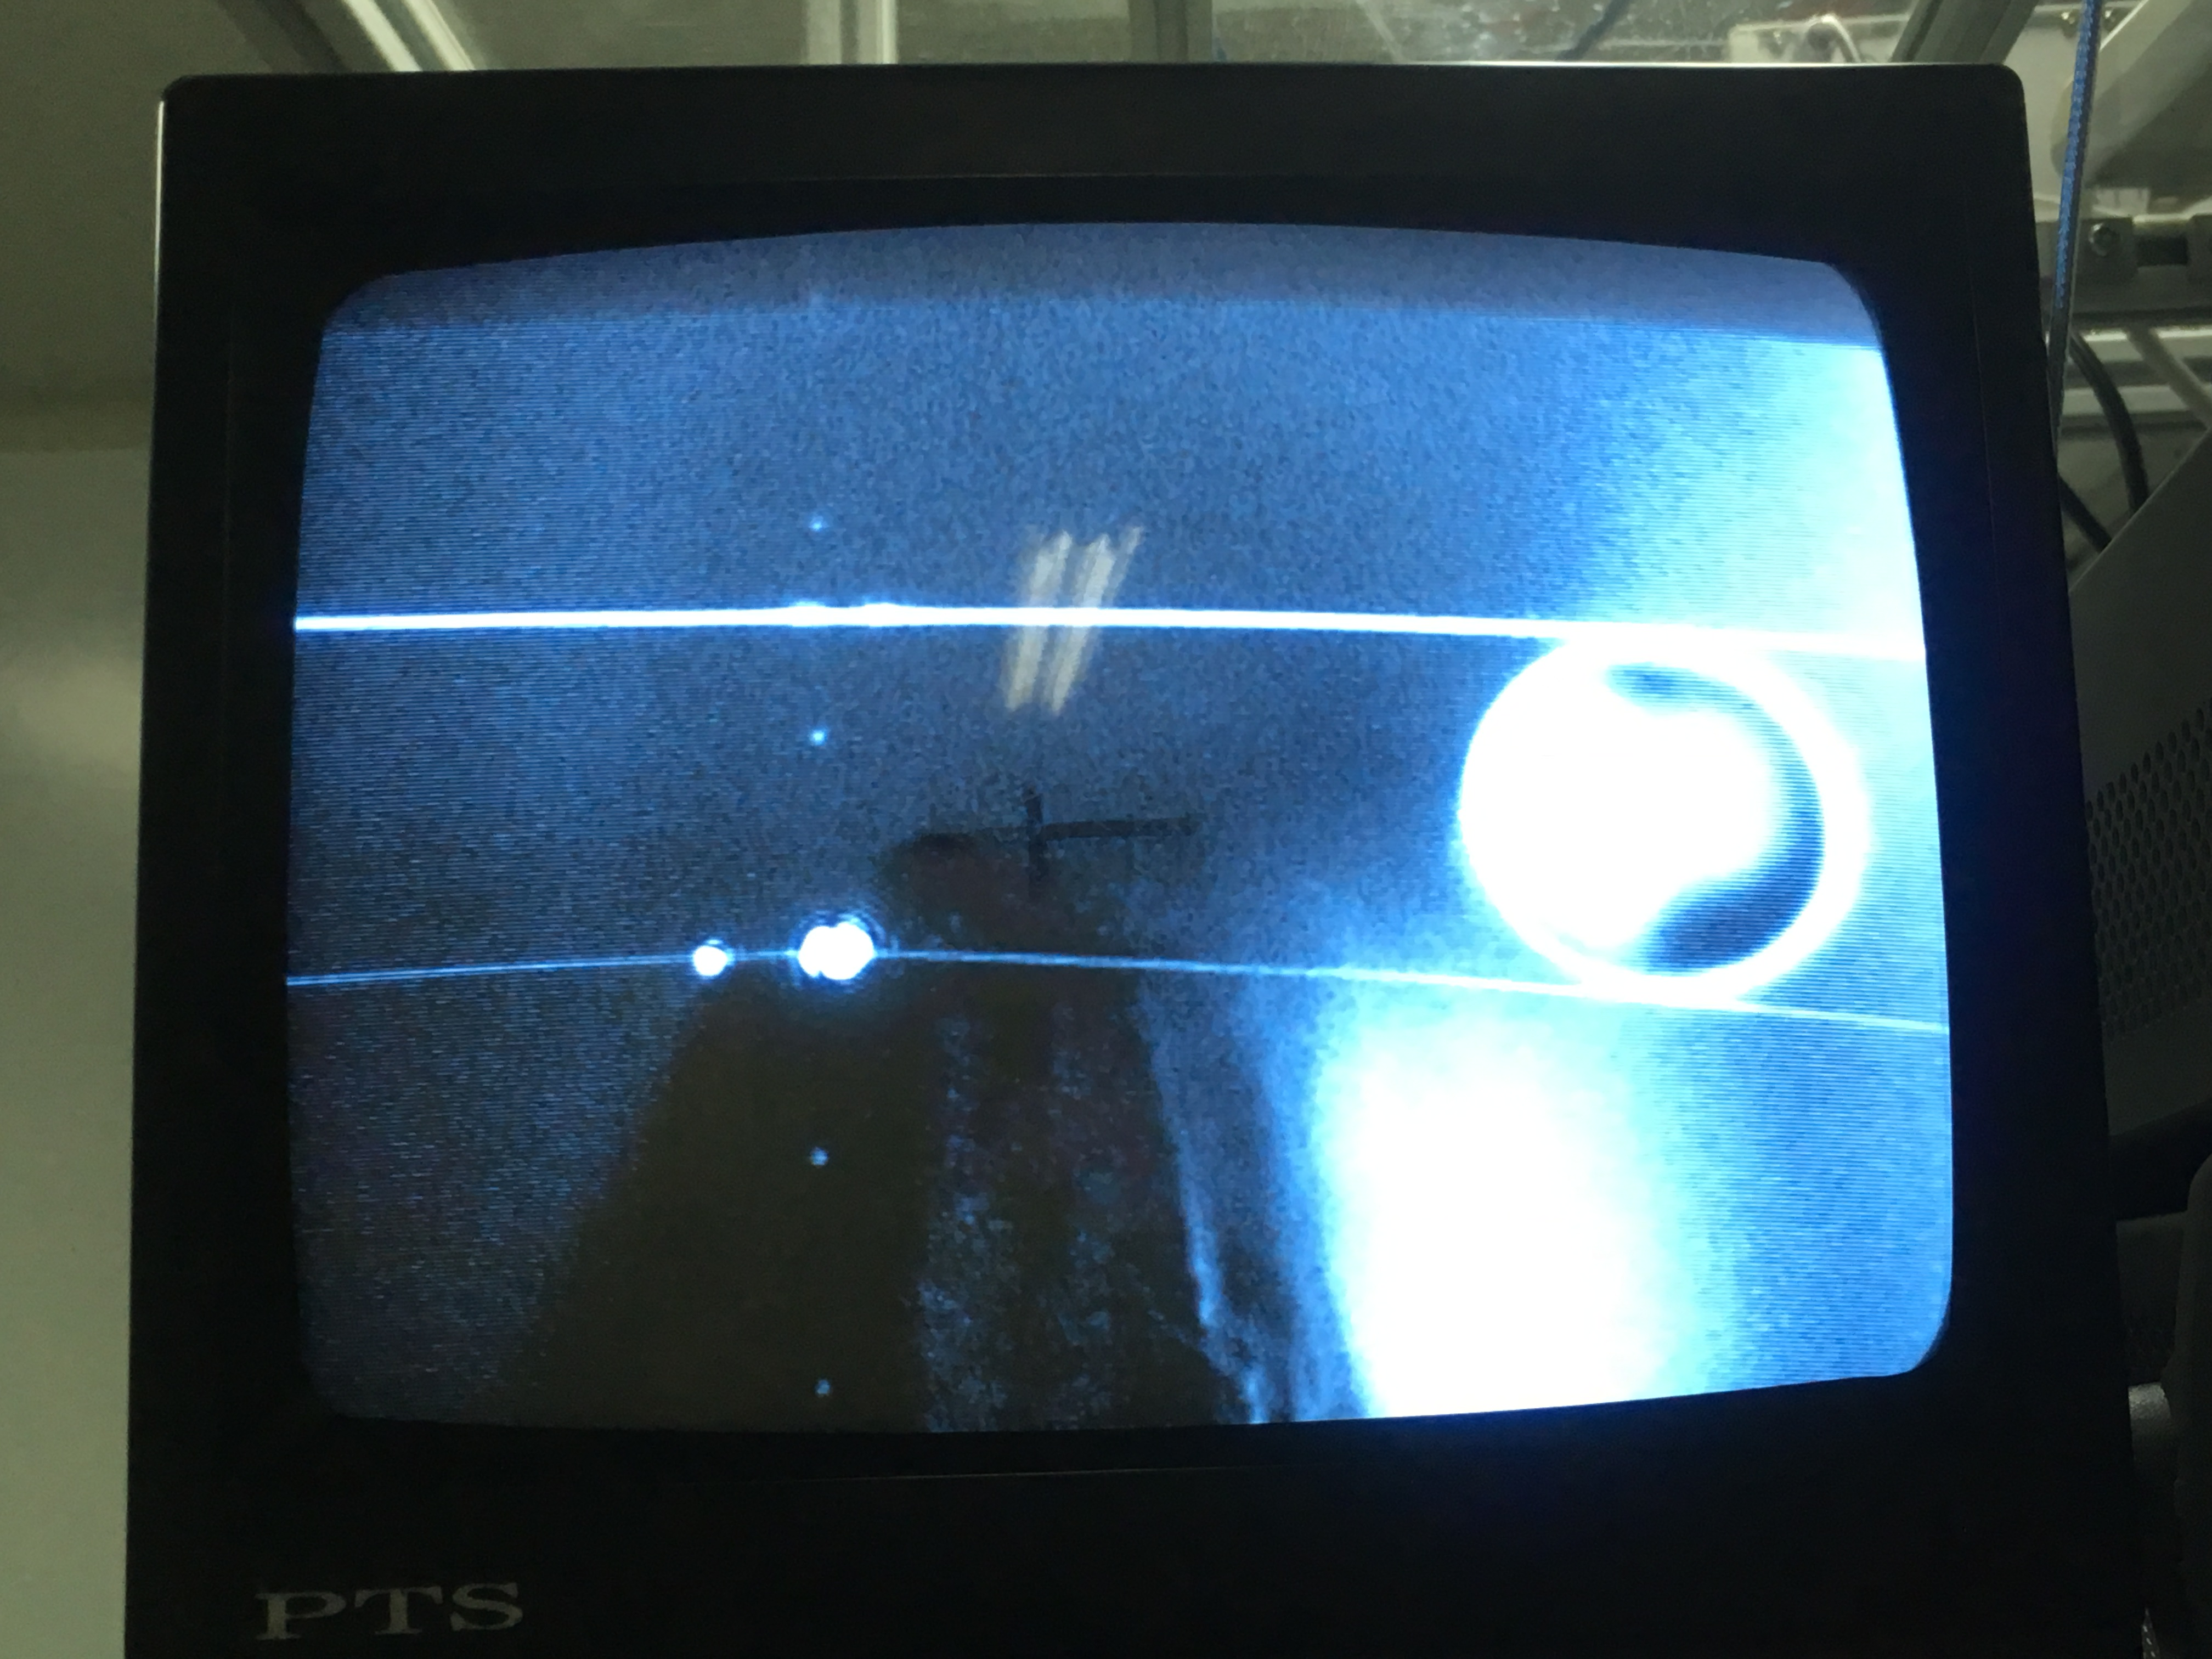
\includegraphics[width=16cm ]{coupling}
\caption{耦合时的光纤锥和微球腔顶视图}
\label{pic:coupling}
\end{figure}

在图\ref{pic:Fiber_sphere}中可以看到,两根光纤间的距离(取决于未去包层的光纤直径)约为250$\mu m$,比微球腔直径大得多,无法进行直接耦合,在实验中,加了一个固定在三维纳米平移台上的尖硅片,用硅片挑住信号光光纤锥,可以调节它与微球腔的相对距离和高度,移到一个合适的位置进行耦合,如图\ref{pic:coupling}所示,左下方阴影为尖硅片。

在实验中,泵浦光光纤在找到了波矢匹配位置之后就保持不动,为了实现较好两个波段的较好耦合,首先将球腔靠近泵浦光光纤锥,通过调节球腔位置并检测投射谱,使其与泵浦光光纤实现临界耦合。调节好球腔位置之后,再通过硅片操纵信号光光纤锥使得它与球腔实现较好耦合,在这个过程中,在信号光光纤中输入778nm附近的激光,通过监测投射谱来监测信号光耦合情况。在采集二次谐波数据时,为了保护EMCCD,输入光光源处于关闭状态。

\newpage
\section{实验结果及分析}
\label{sec:measurement}

\subsection{二次谐波信号的产生及两根光纤锥收集情况对比}

%SH spectrum, pump spectrum, Q, f1f2
\begin{figure}
\centering
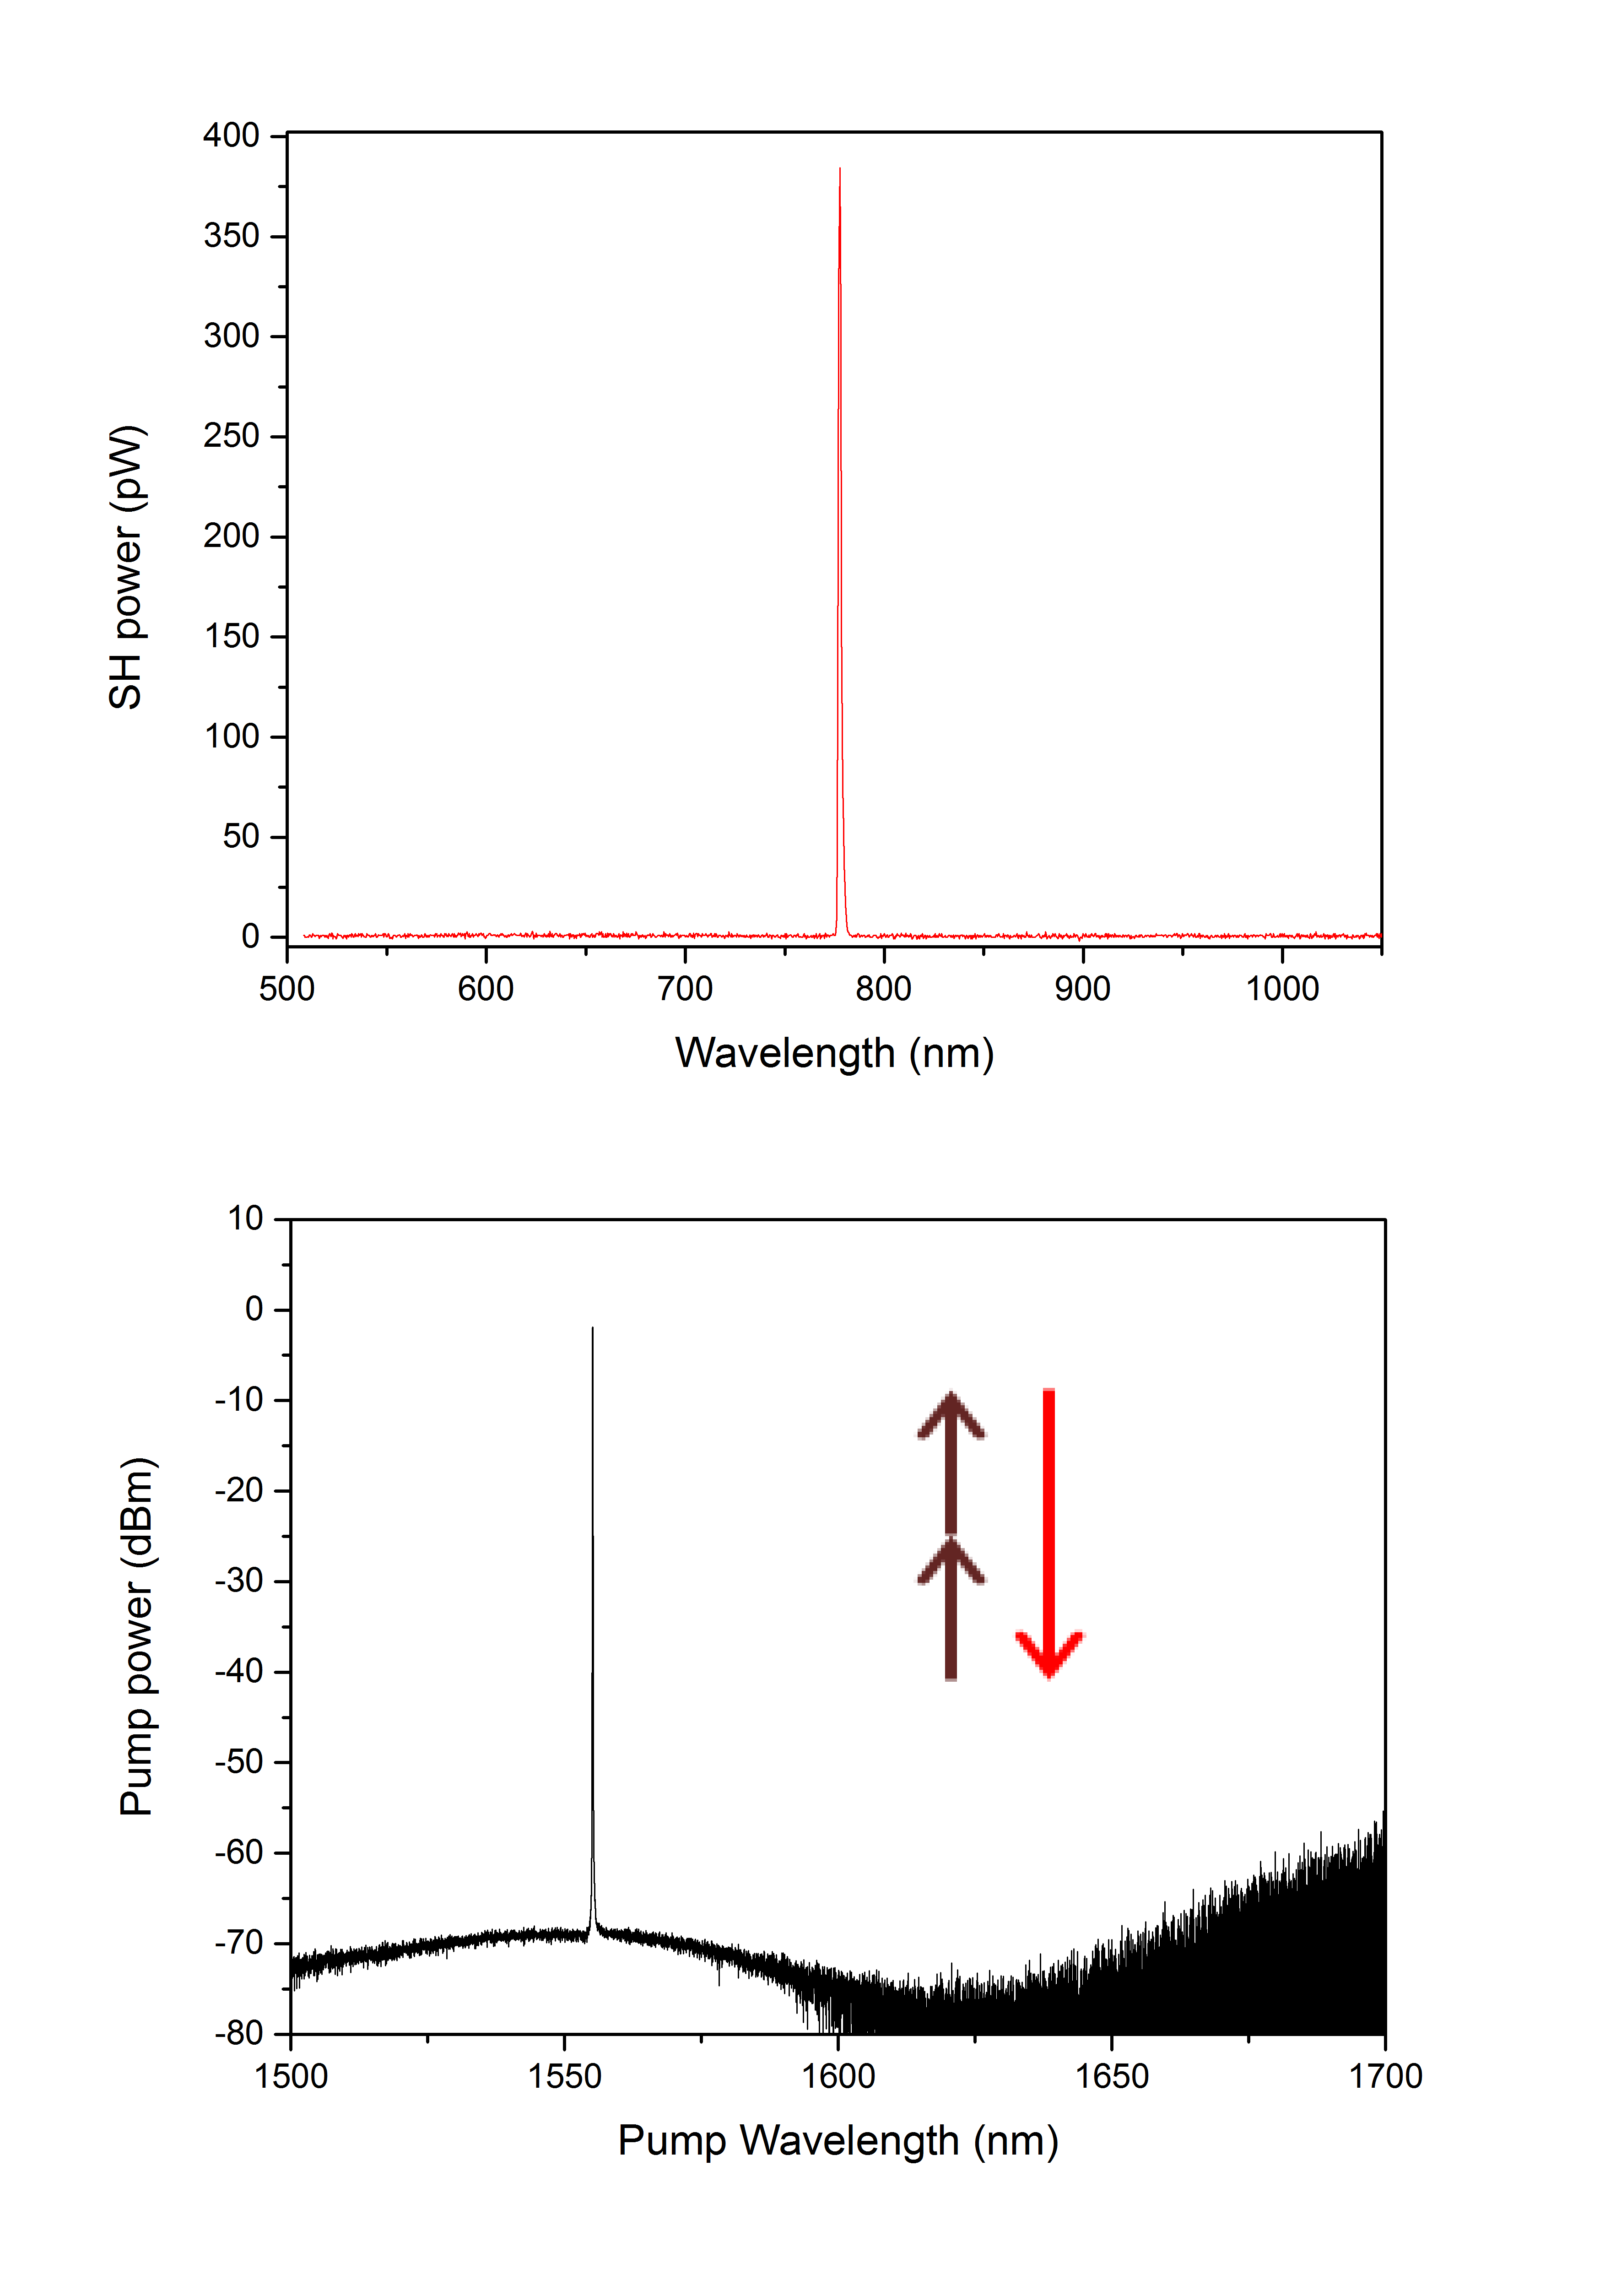
\includegraphics[width=14cm ]{FigSHspectrum}
\caption{二次谐波产生光谱图。上图为二次谐波光谱,下图为泵浦光光谱,插图为二次谐波产生的能级示意图}
\label{pic:FigSHspectrum}
\end{figure}

使用\ref{sec:ExpSetup}中的实验装置,在功率和偏振合适的情况下,可以观察到二次谐波信号,如图\ref{pic:FigSHspectrum}所示,此时的微腔处光纤中泵浦光功率为4.46mW。二次谐波功率的最大值出现在777.75$\pm0.34$nm处,泵浦光功率最大值出现在1555.14nm处,满足二倍频关系。


二次谐波信号与微球腔密切相关,如果将微球腔移开或将微球腔和信号光光纤锥在保持间距不变的情况下一起移开,信号光光纤锥中都不会收集到任何信号。

此外,二次谐波信号还与微球腔的模式密切相关。由于热效应和Kerr效应的影响,在波长逐渐增大耦合进腔膜中时,耦合会逐渐加深,且在较长一段波长范围之内都处在该模式之中,但一旦泵浦光追上腔膜之后,就会跳出该模式,此时反向调节泵浦光,不会立刻进入该模式\cite{carmon2004dynamical},因此可以利用此特性,使得一些波长点只在增加波长调节的过程中在该模式内,而反向调节的过程中,不在该模式内。图\ref{pic:FigSHspectrum}所示的波长满足这样的条件,出模式之后反向调节的过程中在该波长处依然没有进入模式,而在EMCCD上也完全观测不到该图所示的二次谐波信号。由此排除了该信号是光栅二级衍射信号的可能性,因为光栅二级衍射信号只与波长和泵浦光功率有关而与模式无关。

\begin{figure}
\centering
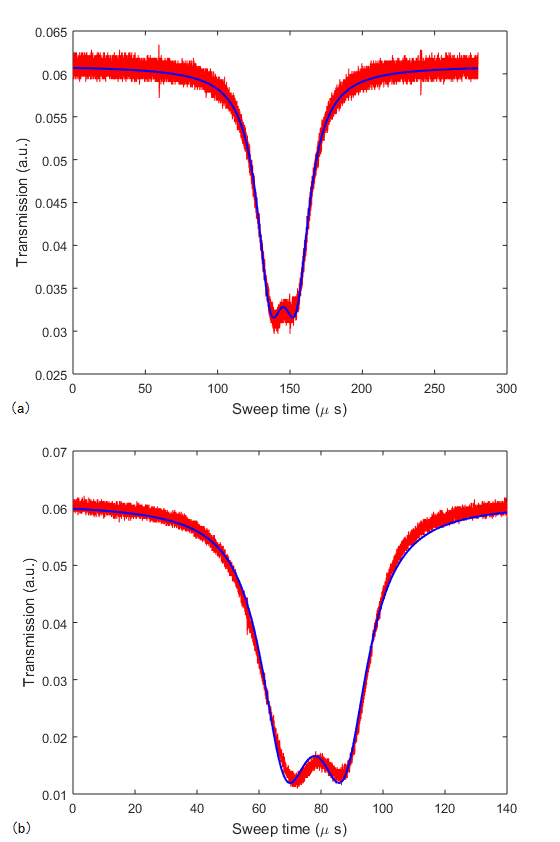
\includegraphics[width=12cm ]{Qfit_w}
\caption{产生二次谐波的模式透射谱。a, 信号光光纤靠近微球腔时的透射谱。b, 信号光光纤移开微球腔时的透射谱。}
\label{pic:Qfit_w}
\end{figure}

为了进一步观察该模式的特性,实验中降低功率到热效应可以忽略,能够看出模式的洛仑兹线形,此时的模式在约1555.02nm处。图\ref{pic:Qfit_w}a是信号光光纤在球腔附近时的模式透射谱,b是信号光光纤远离球腔时的模式透射谱。可以看到该模式存在模式劈裂,这是由于腔表面存在散射点,使得频率简并的正向传播和背向传播的行波模式通过散射点耦合起来,如果将模式正交化处理,则两个新的模式为驻波模式,它们与散射点的相对位置不一样,从而导致模式频率不再简并,而产生劈裂\ref{cao2017experimental},一般在品质因子较高的情况下容易观察到这样的现象。图中的蓝线是理论拟合结果,由该结果可以推知,信号光光纤锥接近球腔时的本征品质因子为3.62$\times 10^7$,而将信号光光纤锥移开时的本征品质因子为4.83$\times 10^7$,这里的本征品质因子是相对于泵浦光光纤锥来说的,即信号光光纤锥的影响也包含在里面。由于信号光光纤锥的存在,使得腔中光场多了一条耗散通道,所以本征品质因子有所降低。

为了证明信号光光纤锥虽然降低了品质因子,但能够提高收集到的二次谐波信号功率。实验中选取了另一个模式,在泵浦光输入功率约7.45mW时进行探测。用图\ref{pic:ExpSetup}所示的实验装置图,在信号光光纤锥中收集到二次谐波信号功率约为5nW。接着将信号光光纤锥移开,将泵浦光光纤锥出口直接接在EMCCD上,仅用泵浦光光纤锥完成信号的激发和收集。直接移开信号光光纤锥,泵浦光光纤锥中收集到的二次谐波信号不足0.1nW,通过纳米平移台精细调节球腔相对泵浦光光纤锥的位置,可以得到一个二次谐波功率的最大值,为0.364nW。可见,信号光光纤锥对于观察二次谐波,尤其是功率较弱的 二次谐波信号具有重要作用。

同样,只用泵浦光光纤锥也进行了正向、反向调节波长的测试,只有在模式中特定位置才能够看到二次谐波信号,如果不在模式中,即使有相同的泵浦光功率和波长,也看不到信号。进一步证明了该信号来自于球腔,而非EMCCD的光栅二级衍射。

\begin{figure}
\centering
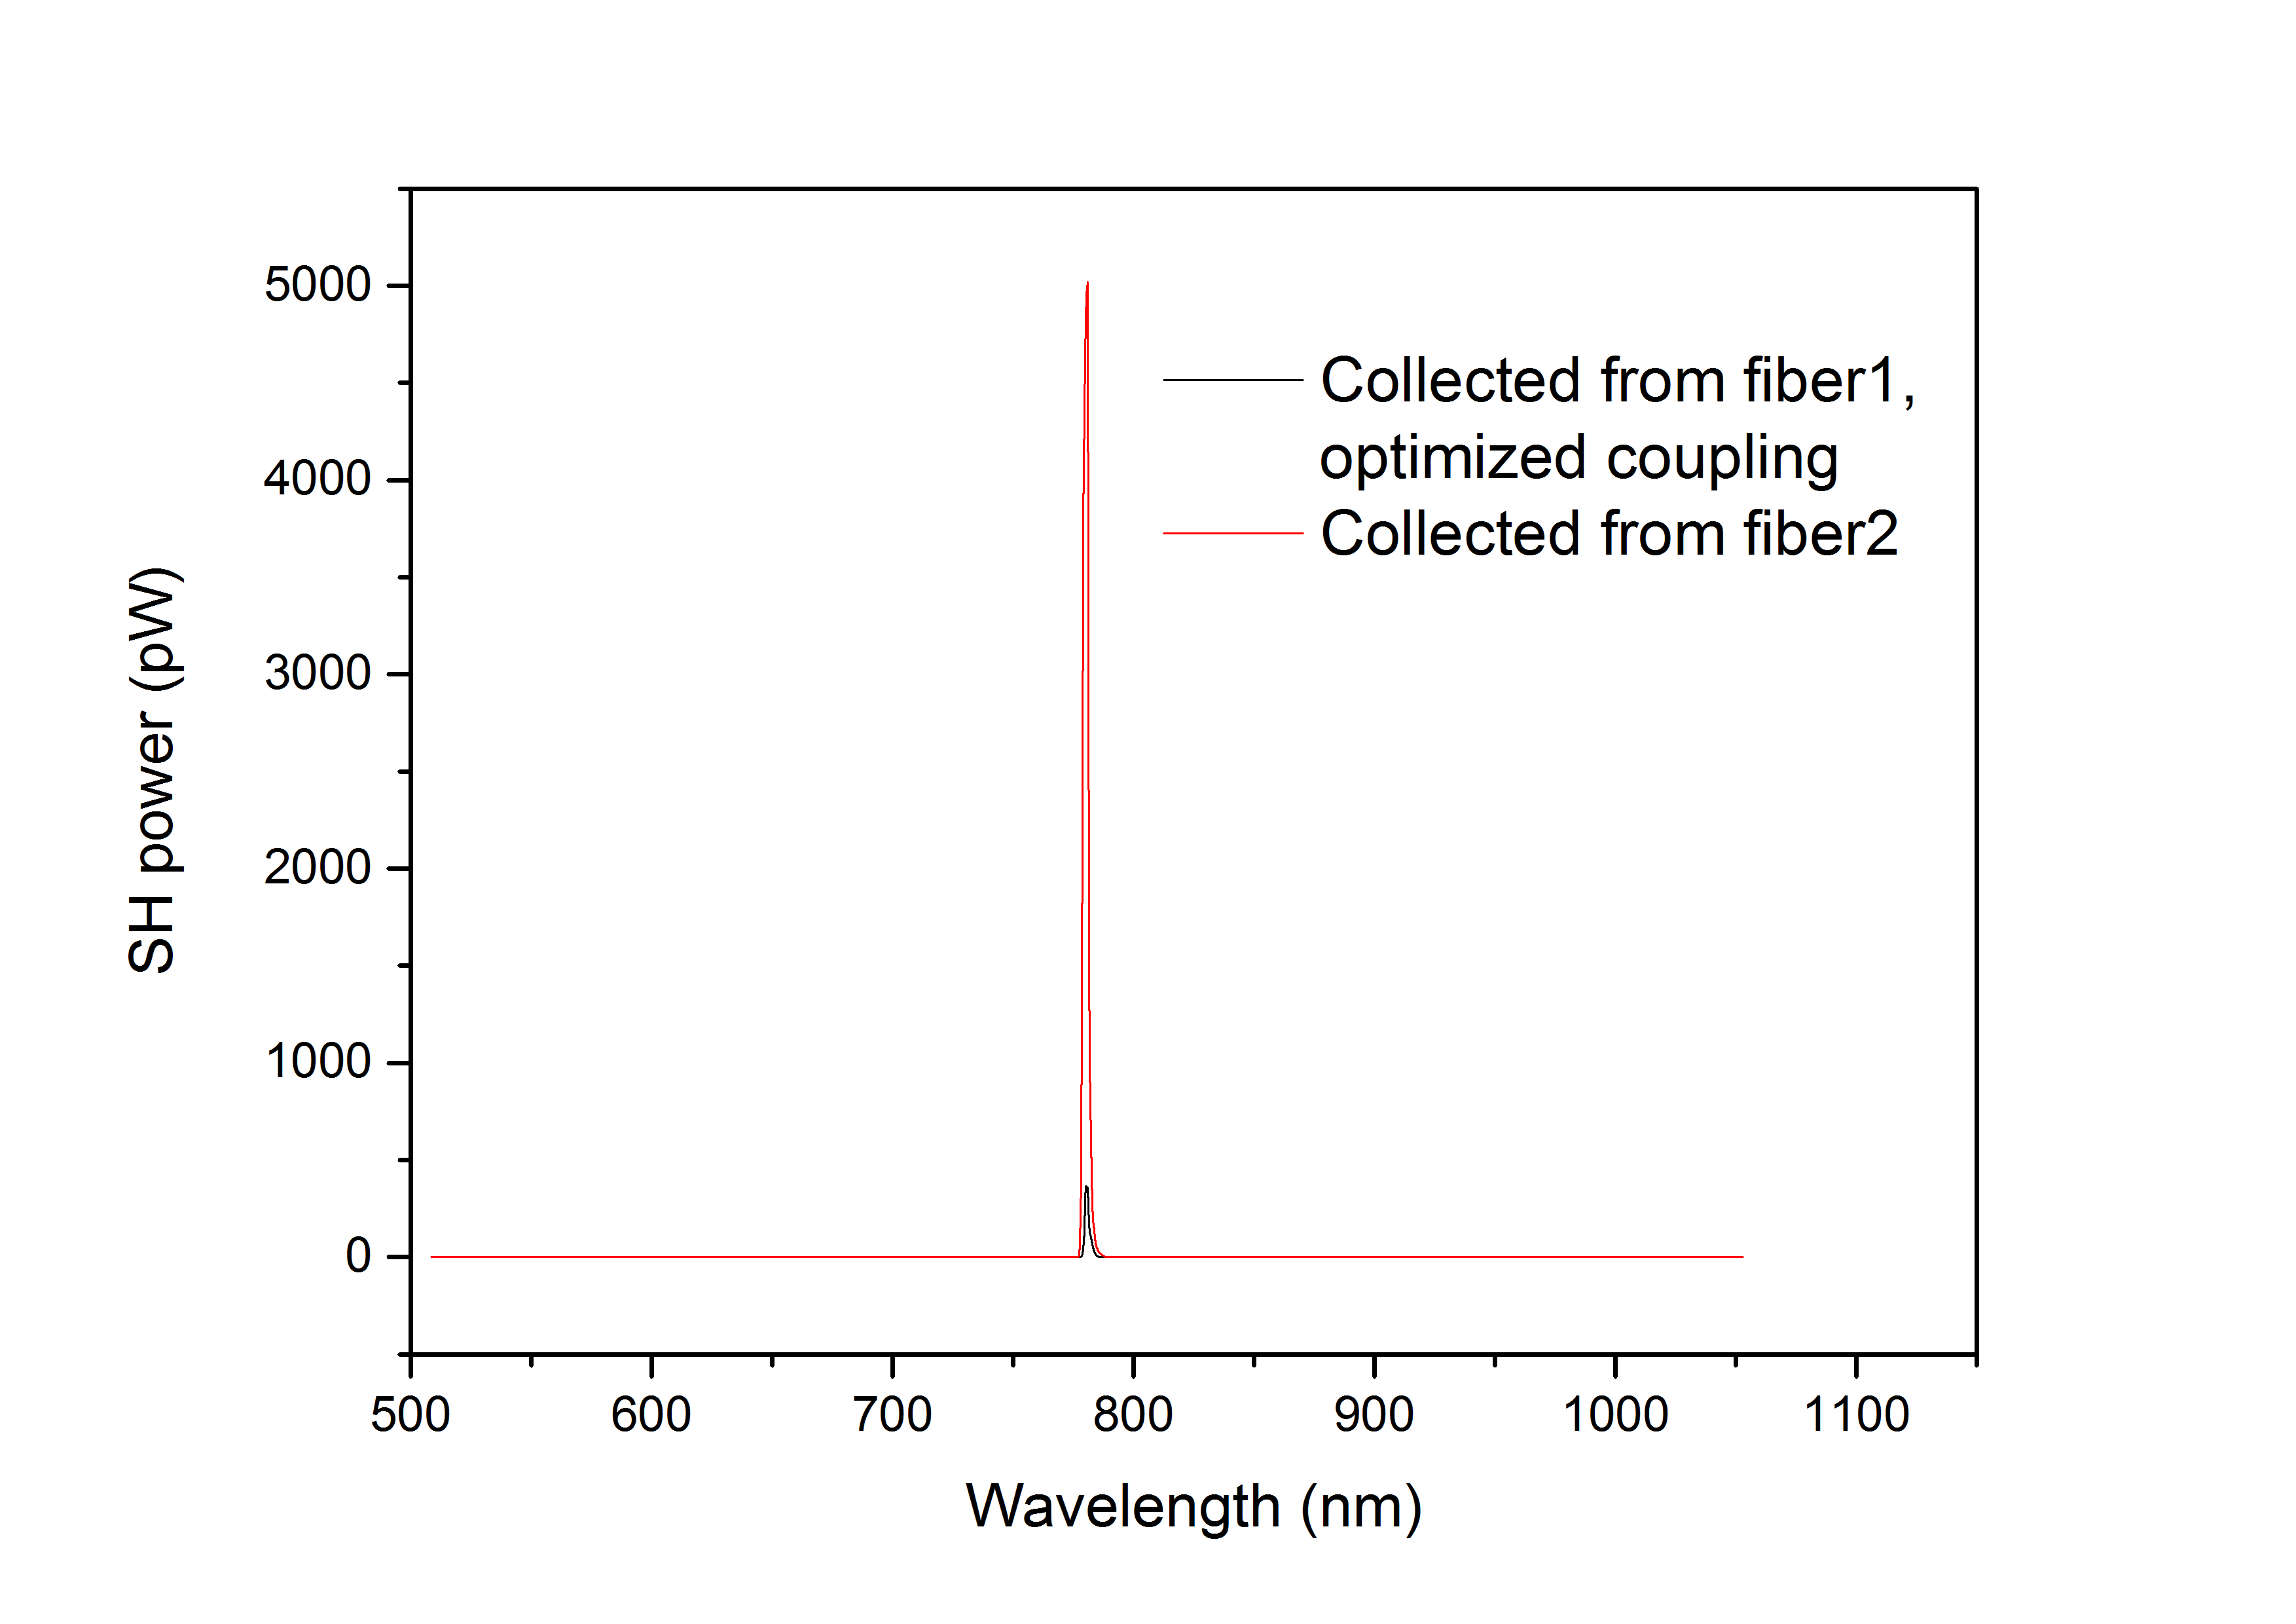
\includegraphics[width=14cm ]{Figf1_f2}
\caption{两根光纤锥收集信号对比,红线为用信号光光纤锥收集到的信号,耦合位置未经过优化,黑线为将信号光光纤锥移开后,只用泵浦光光纤锥在产生二次谐波功率最大的耦合位置收集到的二次谐波信号。}
\label{pic:Figf1_f2}
\end{figure}

\subsection{二次谐波信号对失谐和输入光功率的依赖关系}

%two figures, movement of 780nm, 

\begin{figure}
\centering
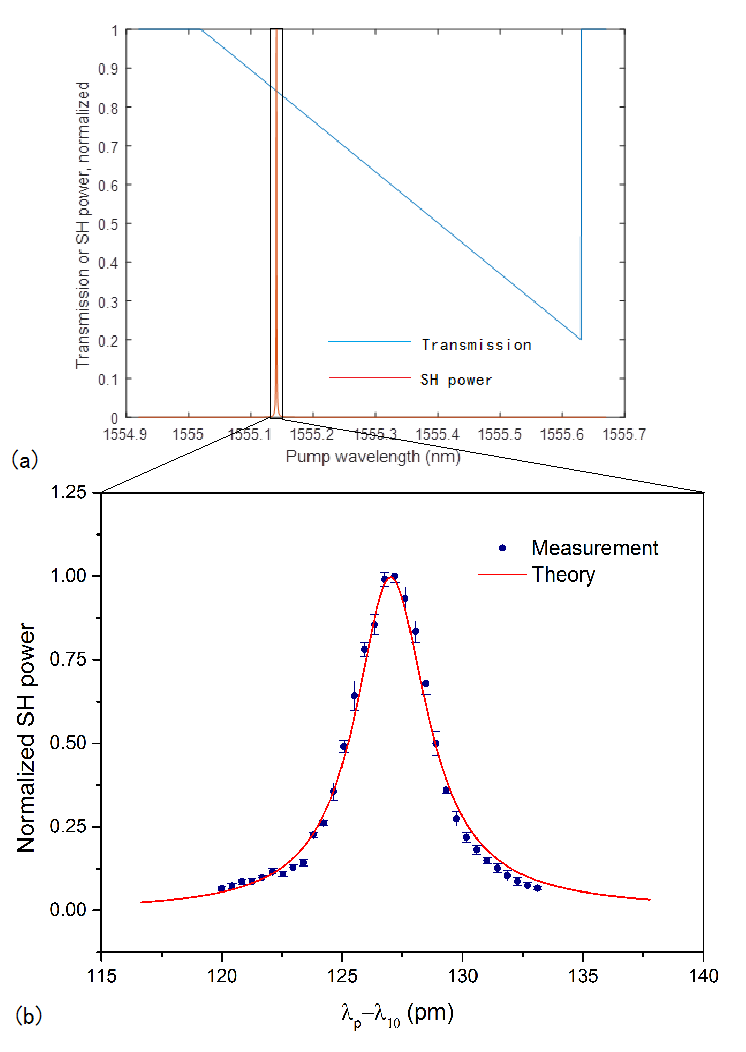
\includegraphics[width=14cm ]{TransSHpower}
\caption{二次谐波信号与失谐的关系。a,归一化的泵浦模式透射谱(波长依次增大)和归一化的二次谐波信号功率随泵浦光波长的变化,理论计算。b,二次谐波功率较大的部分随失谐变化关系。}
\label{pic:TransSHpower}
\end{figure}

图\ref{pic:TransSHpower}展示了二次谐波信号随失谐的变化关系,失谐是泵浦光波长和冷腔模(输入光功率极小,热效应可忽略时的腔膜波长,在本实验中为1555.02nm)之差。a图是以实验中拟合得到的数据作为参数,使用\ref{sec:2Resonance}中的理论得出的泵浦光腔模透射谱和二次谐波功率随泵浦光波长变化的曲线。透射谱由于热效应和Kerr效应,展宽成为一个三角形\cite{carmon2004dynamical},由于此时腔模处于欠耦合状态,故透射谱最低点不到零。根据双共振条件的理论,在泵浦光波长约1555.3nm附近泵浦光波长的一半与二次谐波模式达到共振,因而二次谐波模式产生了一个极大值。

b图展示了二次谐波功率极大值附近的情况,同样使用\ref{sec:2Resonance}中的理论进行拟合,可以得出如下关系,
\begin{equation}
\frac{\kappa_{2e}+\kappa_{20}}{2} = (2-D_{12})\times 306.5\mathrm{ MHz}
\end{equation}

其中$D_{12}$是单位泵浦光频率变化带来的二次谐波模式频率移动。由于实验上无法确定二次谐波的具体模式,故无法进一步确认$\kappa_2$和$D_{12}$的值。

\begin{figure}
\centering
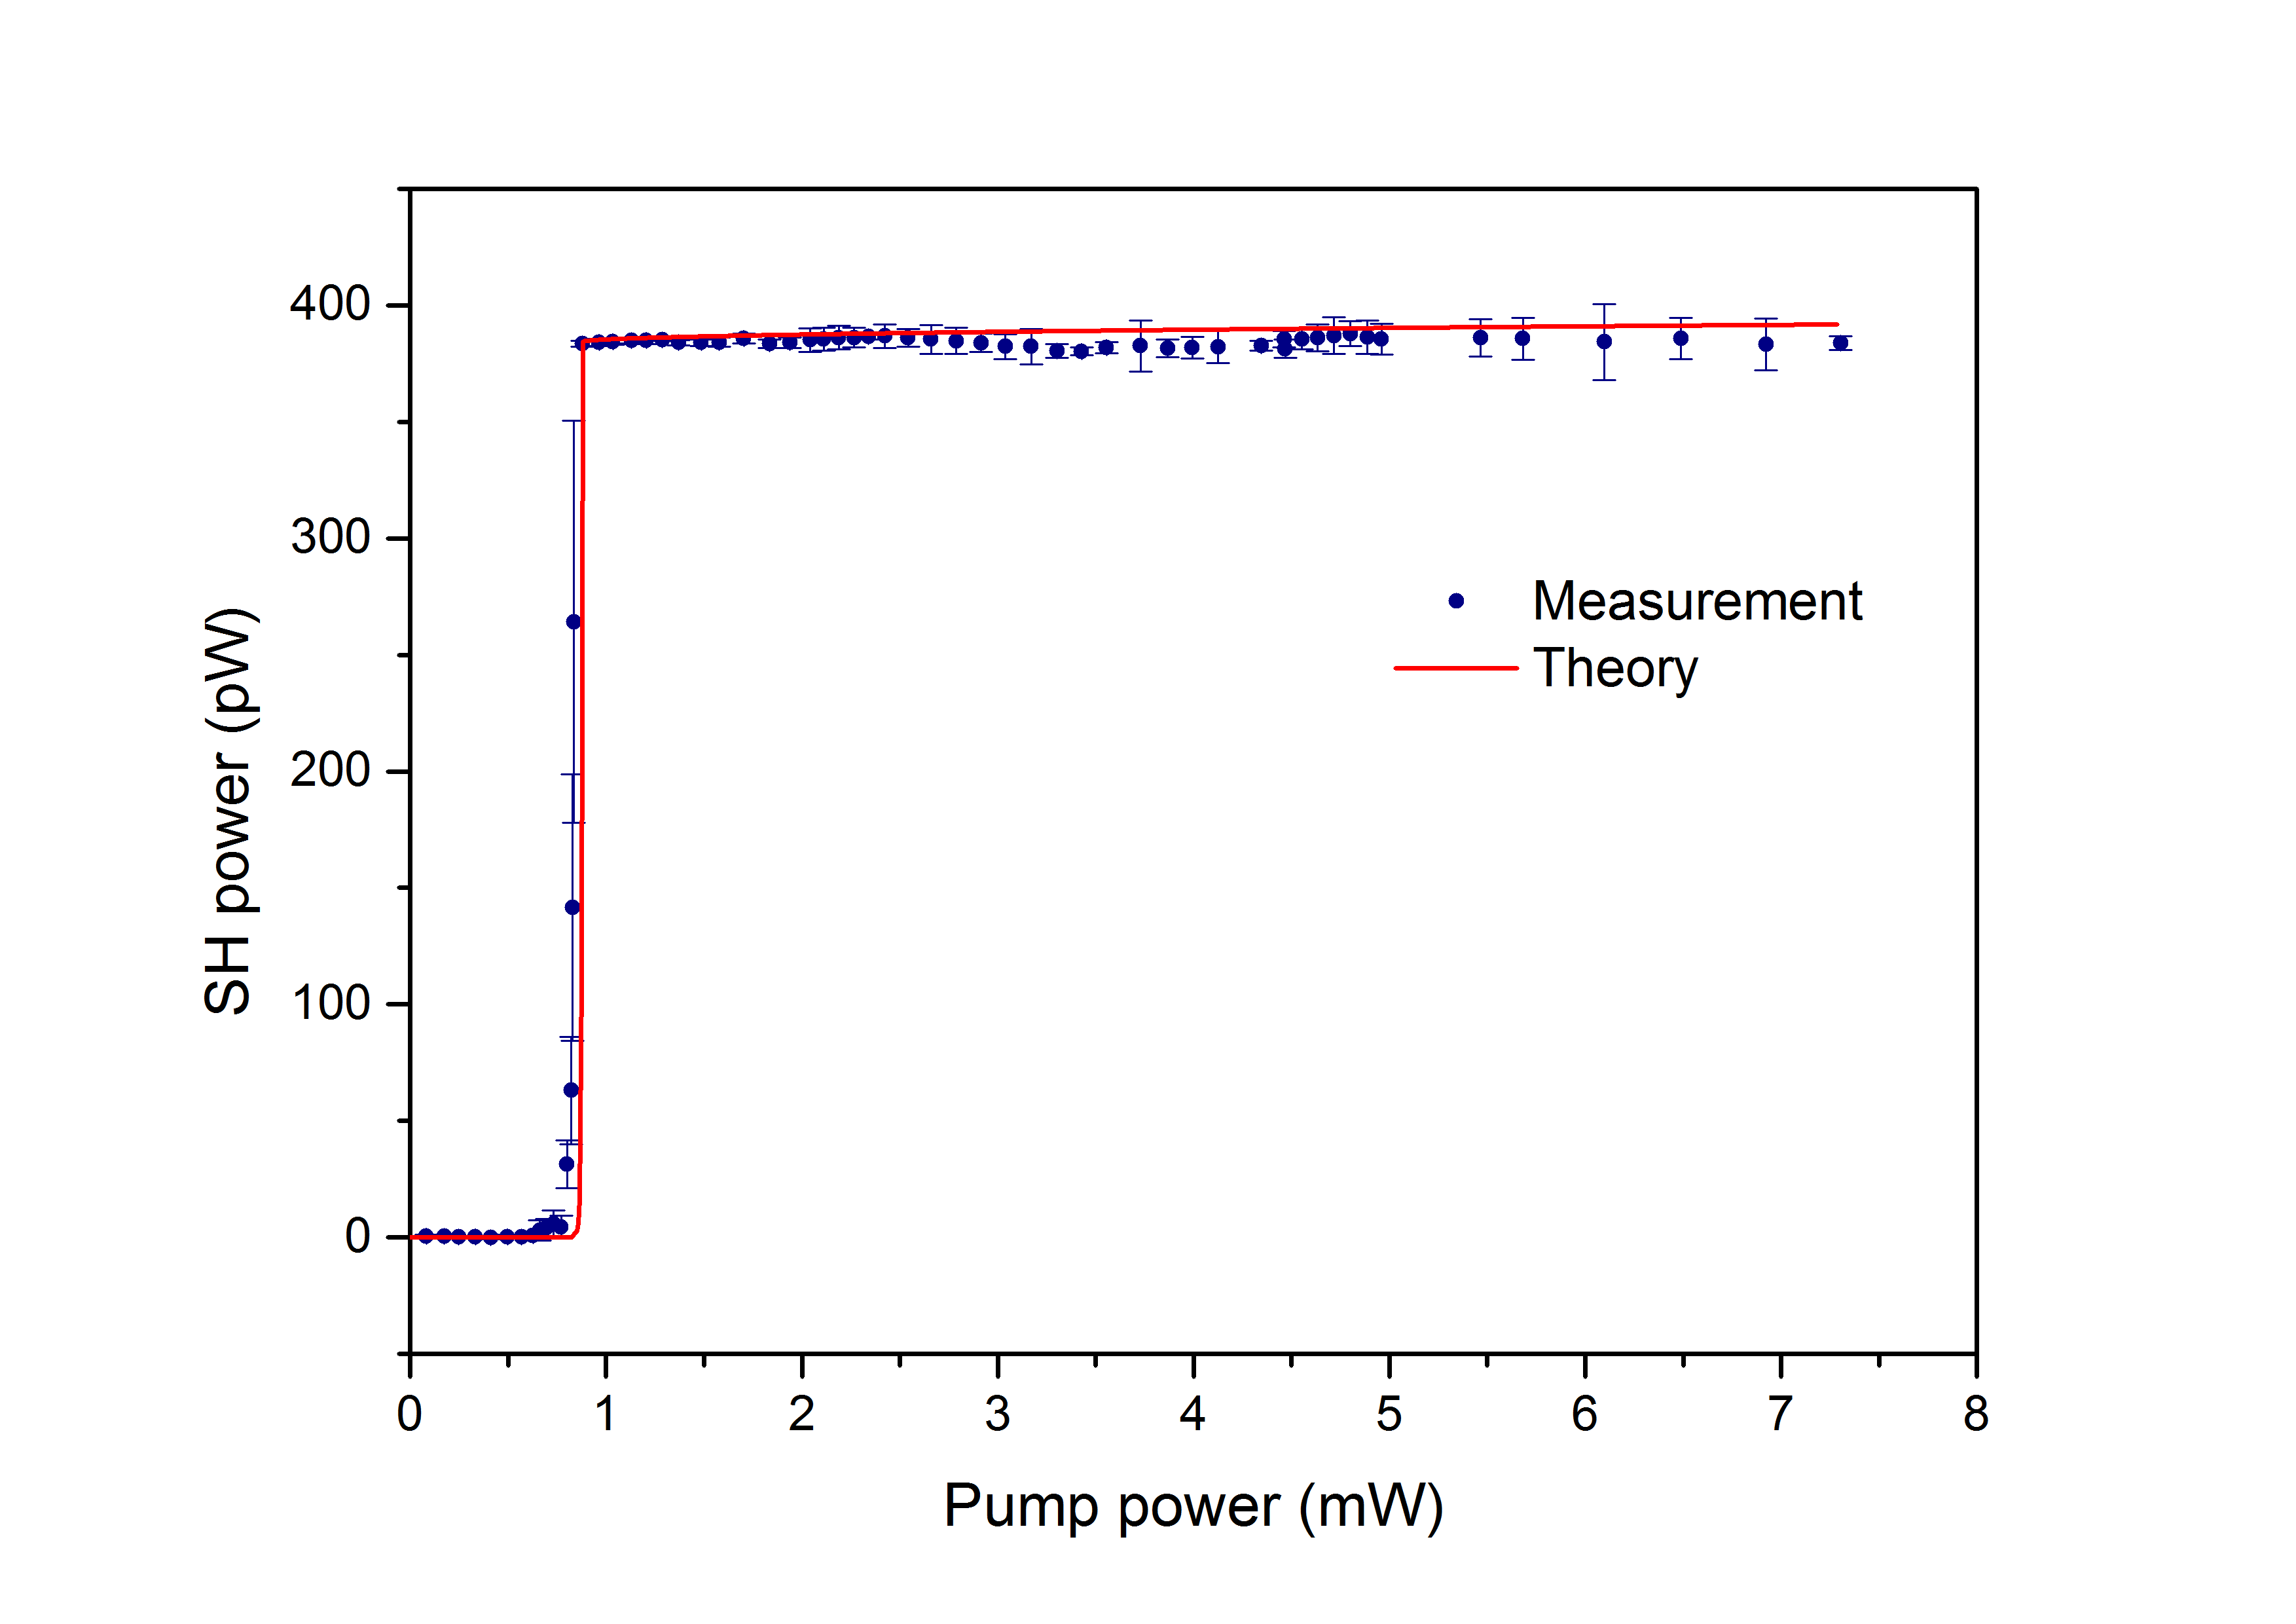
\includegraphics[width=14cm ]{FigSHpower-inputPw}
\caption{二次谐波信号与泵浦光功率的关系。蓝点为实验数据,红线为理论拟合曲线}
\label{pic:FigSHpower-inputPw}
\end{figure}

图\ref{pic:FigSHpower-inputPw}所示为二次谐波信号与泵浦光功率的关系,与图\ref{pic:P2change_ed2_ai}所示的理论预测非常接近。实验数据是固定一个泵浦光功率之后,向波长增大的方向扫描泵浦光波长,由上文分析的二次谐波功率随失谐的变化关系,二次谐波功率会逐渐增加,但如果功率较小,使得还未达到二次谐波功率较大的时候,泵浦光就已经追上腔模,之后会跳出腔模,则二次谐波功率极小。当泵浦光功率逐渐增大,直到能够覆盖使二次谐波功率较大的失谐时,二次谐波最大功率先是在即将失稳处(即泵浦光追上腔模)达到所有失谐中的最大值(固定泵浦光功率不变)。当泵浦光功率增大到能够取到的失谐范围覆盖了二次谐波功率极大值(即图\ref{pic:TransSHpower}b中的峰值),二次谐波功率的最大值每次都是在该峰值处读取,又由于不改变失谐而直接改变泵浦光功率对于腔内能量的增加作用极小,因而此后二次谐波功率极大值随着泵浦功率的增加变化不是很大。

\subsection{二次谐波信号对偏振的依赖关系}

%polarization figure, theories, 
\begin{figure}
\centering
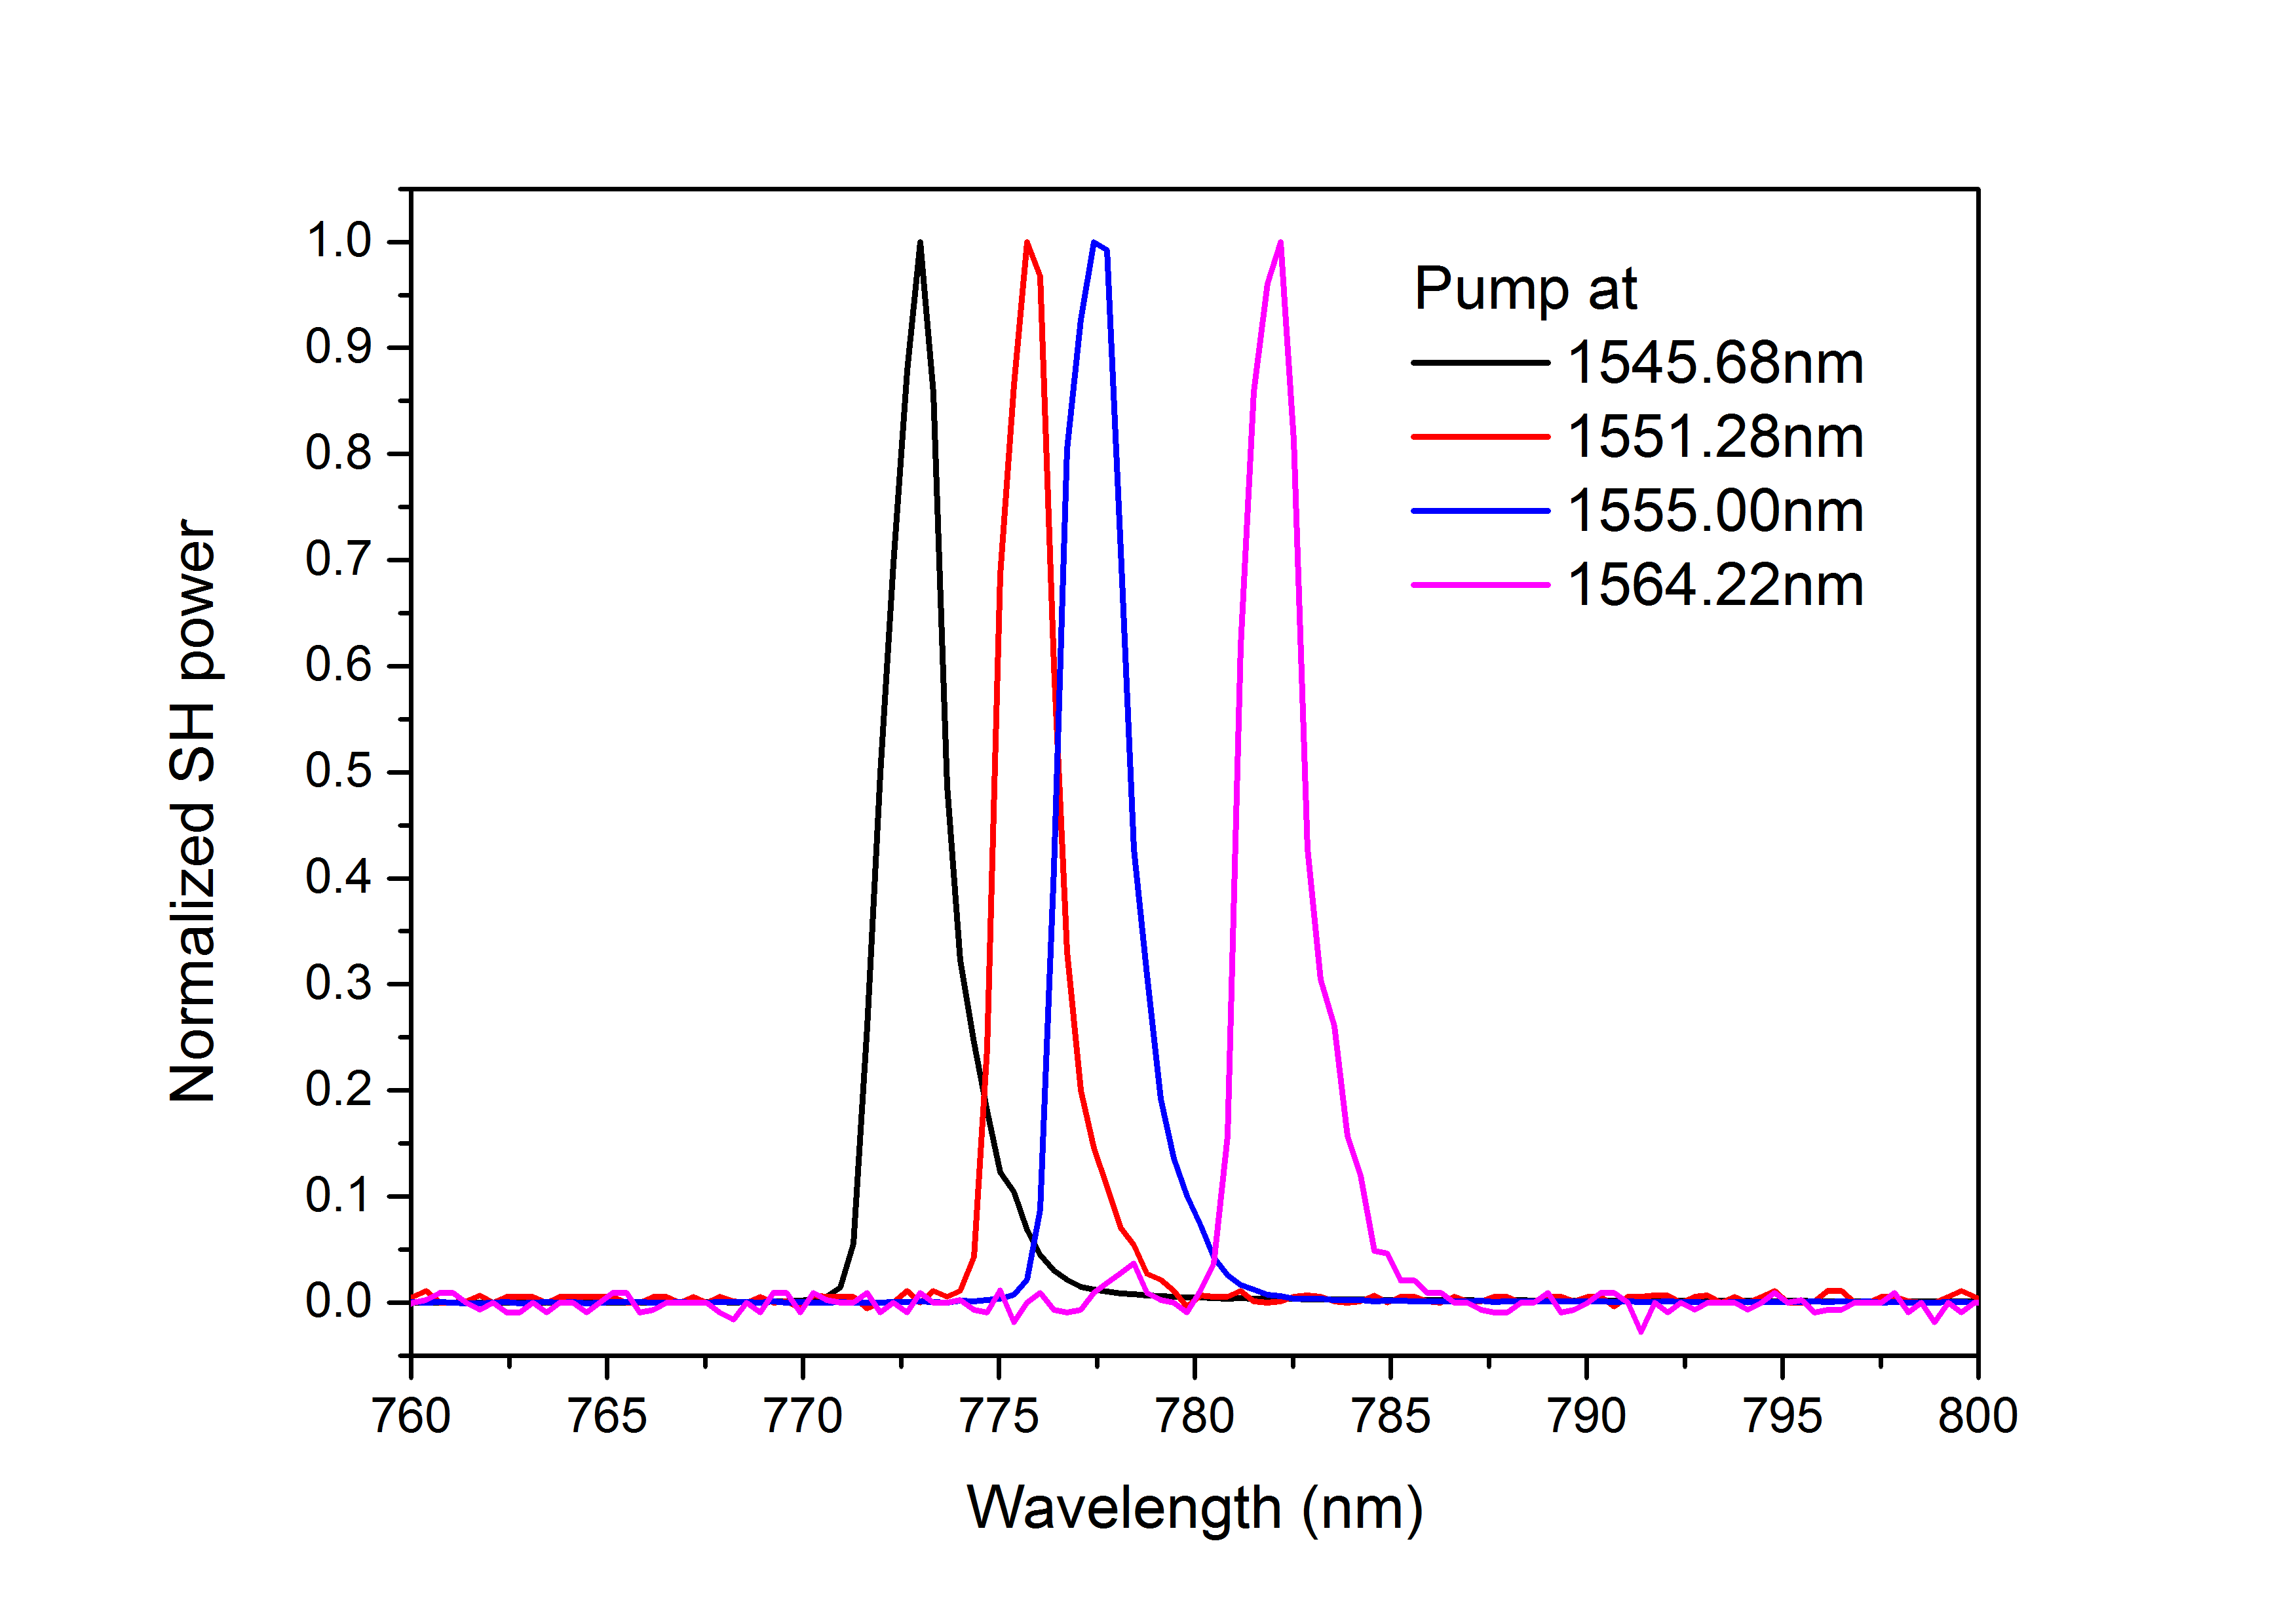
\includegraphics[width=14cm ]{FigSHexamples}
\caption{不同模式产生的二次谐波信号,强度已经归一化。}
\label{pic:FigSHexamples}
\end{figure}

除了上面看到的两个模式产生二次谐波以外,微球腔中还有许多其他不同模式也可以产生二次谐波,实验中泵浦光波长从1545nm到1565nm区间内扫描(超过两个自由光谱范围),整个区间内均有模式能产生二次谐波,如图\ref{pic:FigSHexamples}所示,产生的二次谐波波长也覆盖了773nm至782nm的范围。

针对两个不同的模式比较它们的二次谐波强度没有直接意义,但由于可以观察到很多产生二次谐波的模式,可以研究二次谐波产生的统计特性,其中一个重要方面在于,对于偏振的依赖性。但在本实验中无法直接判别模式是TE还是TM偏振,只能标记为偏振1和偏振2,其中图\ref{pic:FigSHspectrum}所示的模式来自偏振1.实验中,以7.45mW的输入光功率分别采用两种偏振对1545nm到1565nm区间进行了三次扫描,记录下每个对应模式产生二次谐波的最大值,绘制成如图\ref{pic:PolarizationHistogram}所示的统计直方图。由该图可以看出,偏振1对应的模式能够产生更多功率更高的二次谐波,即两个偏振对于产生二次谐波来说并不是平等的。

\begin{figure}
\centering
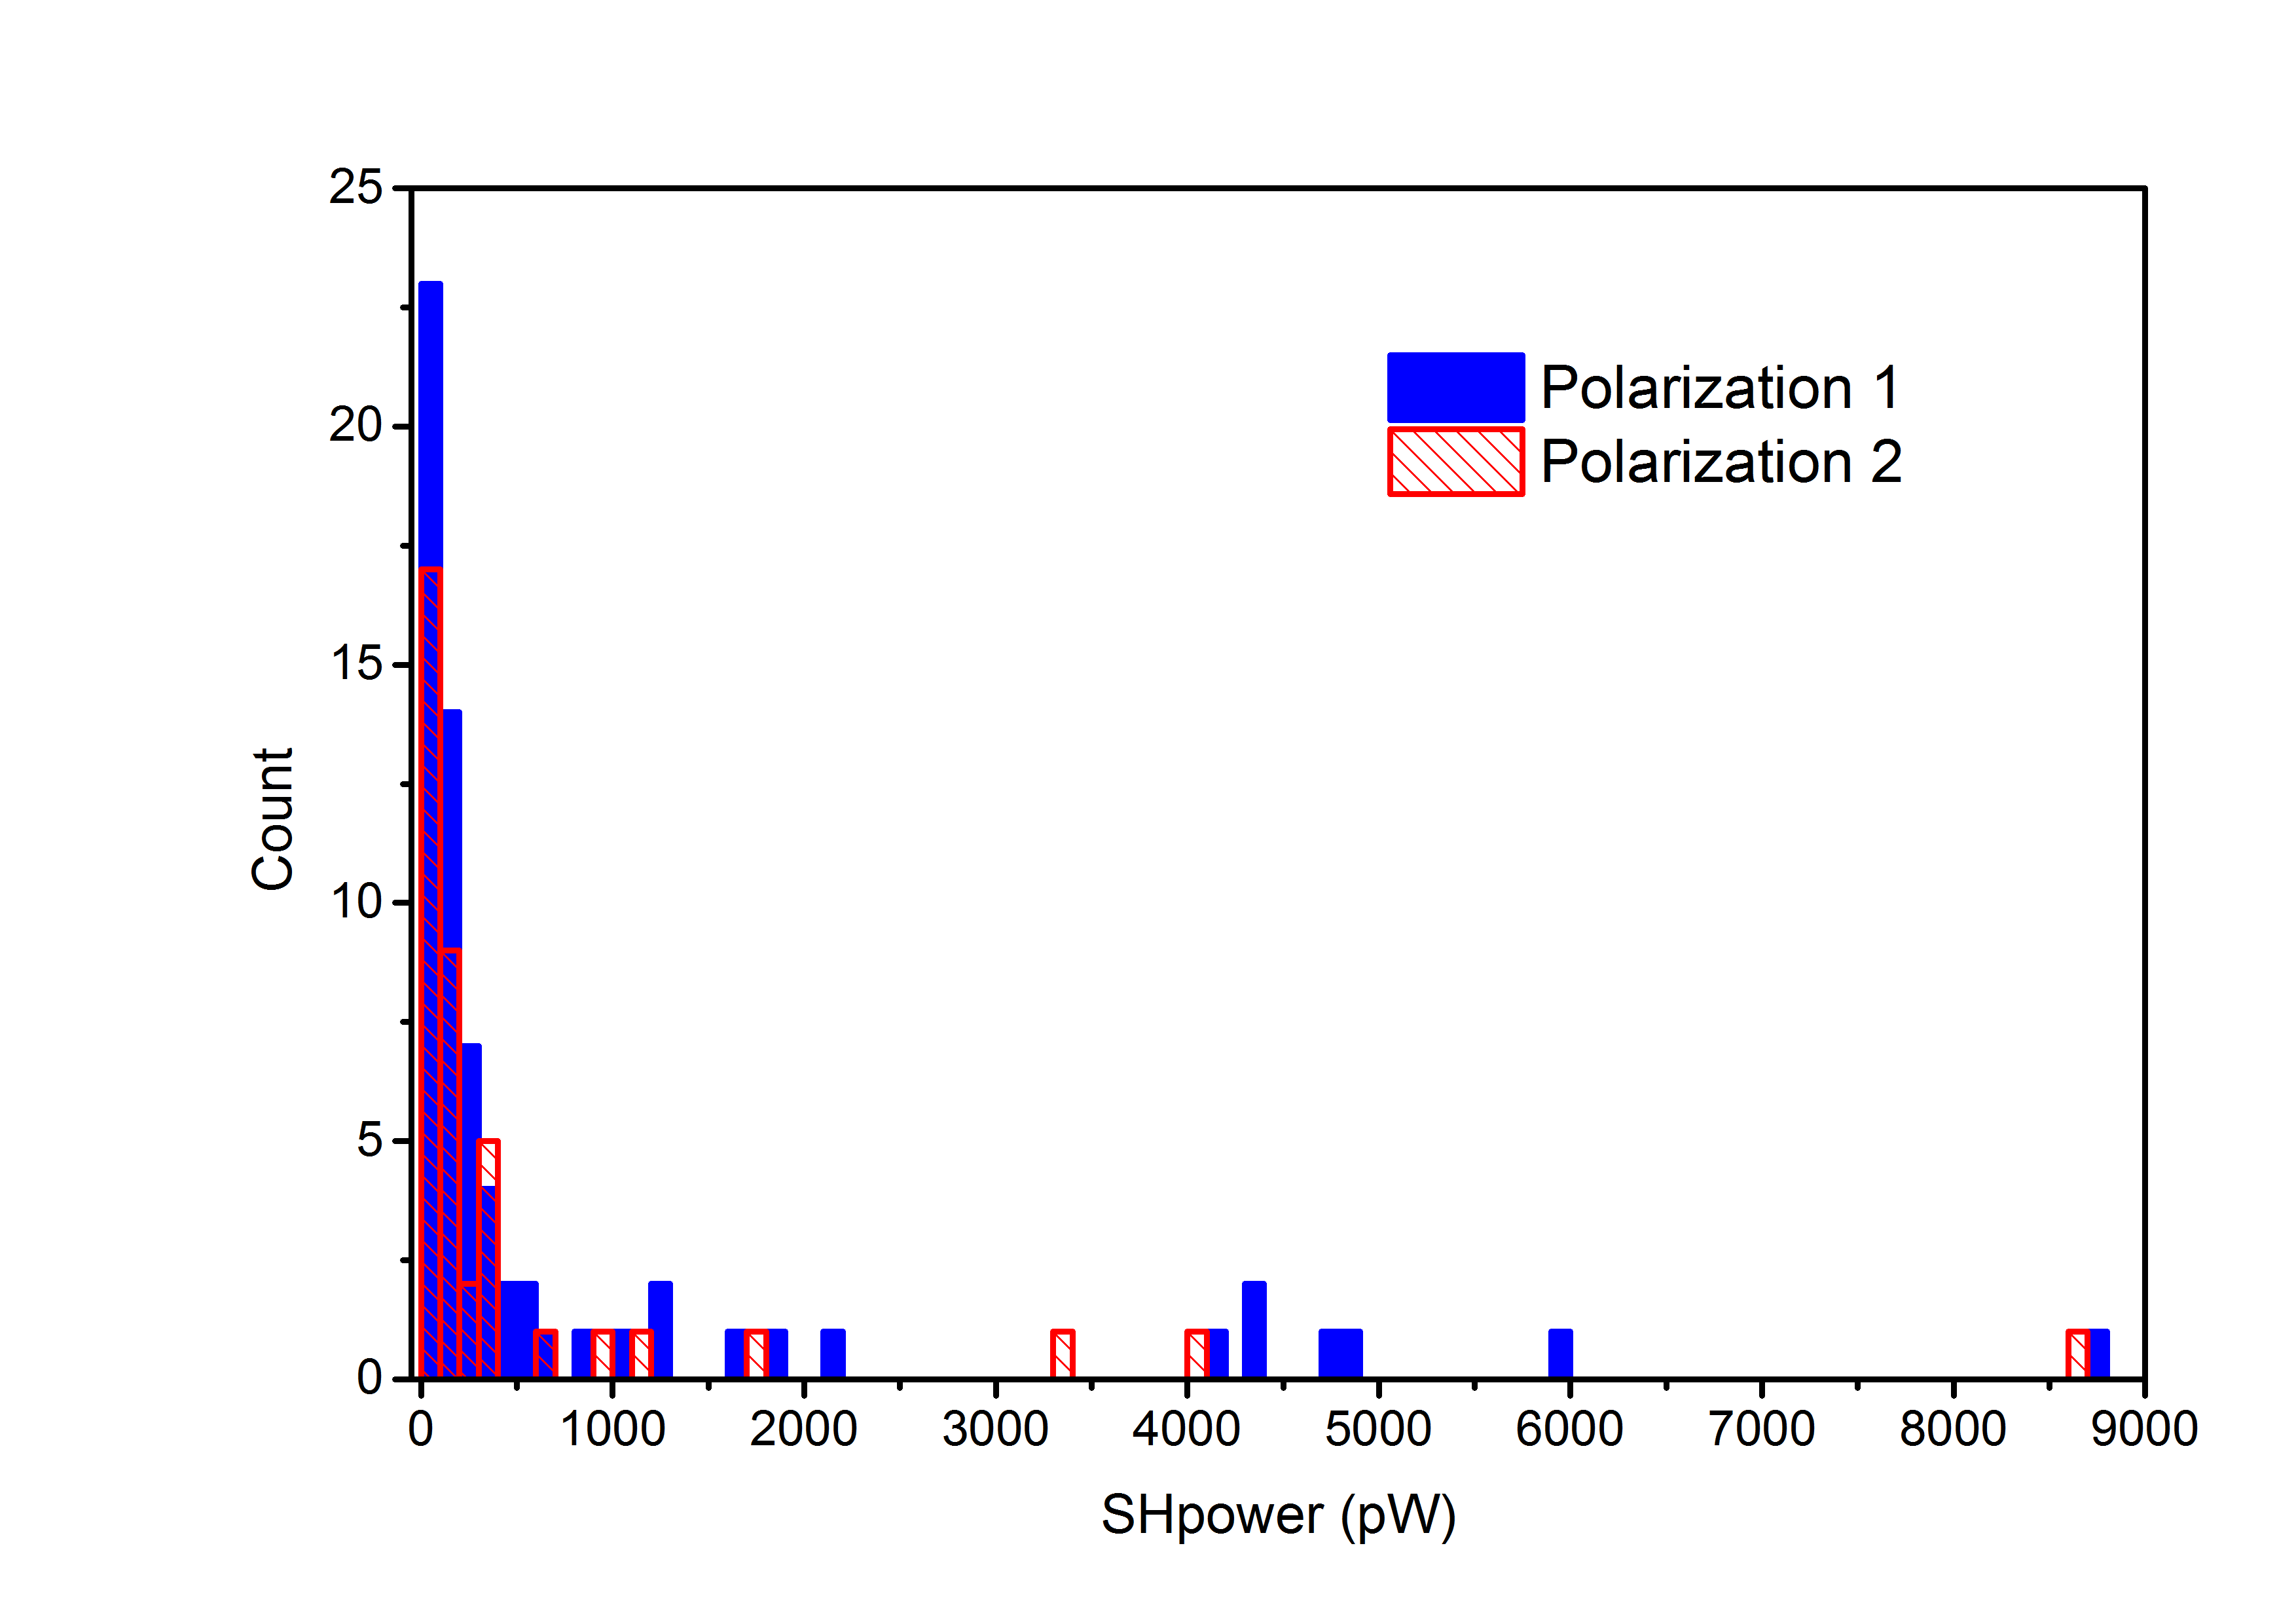
\includegraphics[width=14cm ]{PolarizationHistogram}
\caption{不同偏振中模式产生二次谐波的统计直方图}
\label{pic:PolarizationHistogram}
\end{figure}

解释这个现象需要考虑二氧化硅微球腔中二次非线性的来源。首先考虑表面对称性破缺引起的二次非线性,在非晶态材料当中,表面二次非线性系数是一个张量,只有三个分量不为零,分别是$\chi_{\perp \perp \perp}$,$\chi_{\perp \parallel \parallel}$和$\chi_{\parallel \parallel \perp}$,对于二氧化硅来说,三个系数分别为59,3.8和7.9(单位均为$\times 10^{-22} m^2/V$)。在微球腔中,$\chi_{\perp \perp \perp}$,主要对应着泵浦光和二次谐波均为TM模式,$\chi_{\perp \parallel \parallel}$对应着一个TE泵浦模式的光子和一个TM泵浦模式的光子结合产生了一个TE模式的二次谐波光子,一般这是一个二次合频过程而非二倍频过程,由于本实验只使用一台泵浦光激光器,故不研究此过程。$\chi_{\parallel \parallel \perp}$则对应着两个TE模式的泵浦光子结合产生一个TM模式的二次谐波光子。从系数大小上来看,TM泵浦产生二次谐波的效率应当最高。

另一个二次非线性的来源是体多极效应。由式\ref{eq:gb}可知,体非线性系数为一个标量,而积分中含有空间散度,故这个等效体二次非线性系数与模式的空间分布密切相关。对于TM模式来说,由于电场主要分布在$\mathbf{\hat{r}} $向,故微分也是在这个方向。$\mathbf{\hat{r}} $向本身不存在对称性,因而微分之后与二次谐波模式的电场及泵浦模式电场的乘积空间积分不会为零。TE模式的电场分布在$\mathbf{\hat{\theta}} $向,由于球对称性,这个方向本身也具有对称性,如果泵浦光选取TE角向基模,即,$m=l$,对于角向为偶函数,微分之后是奇函数,而根据\ref{sec:2Resonance}中的积分不为零条件和$M\le L$,二次谐波模式也只能为TE角向基模,为角向偶函数,因而整体的交叠积分为零,即,TE角向基模不能通过体二次非线性产生二次谐波。泵浦光与二次谐波模式都为TE角向二阶模时,空间积分不为零,可以产生二次谐波。另外需要注意的是,无论哪种二次非线性来源,都需要通过径向高阶模式(在实验考虑的条件下为径向二阶模式)来达到初步双共振条件。图\ref{pic:TM1zoomwarrow_1_9319}所示为通过体二次非线性能够产生二次谐波的最低阶模式。

\begin{figure}
\centering
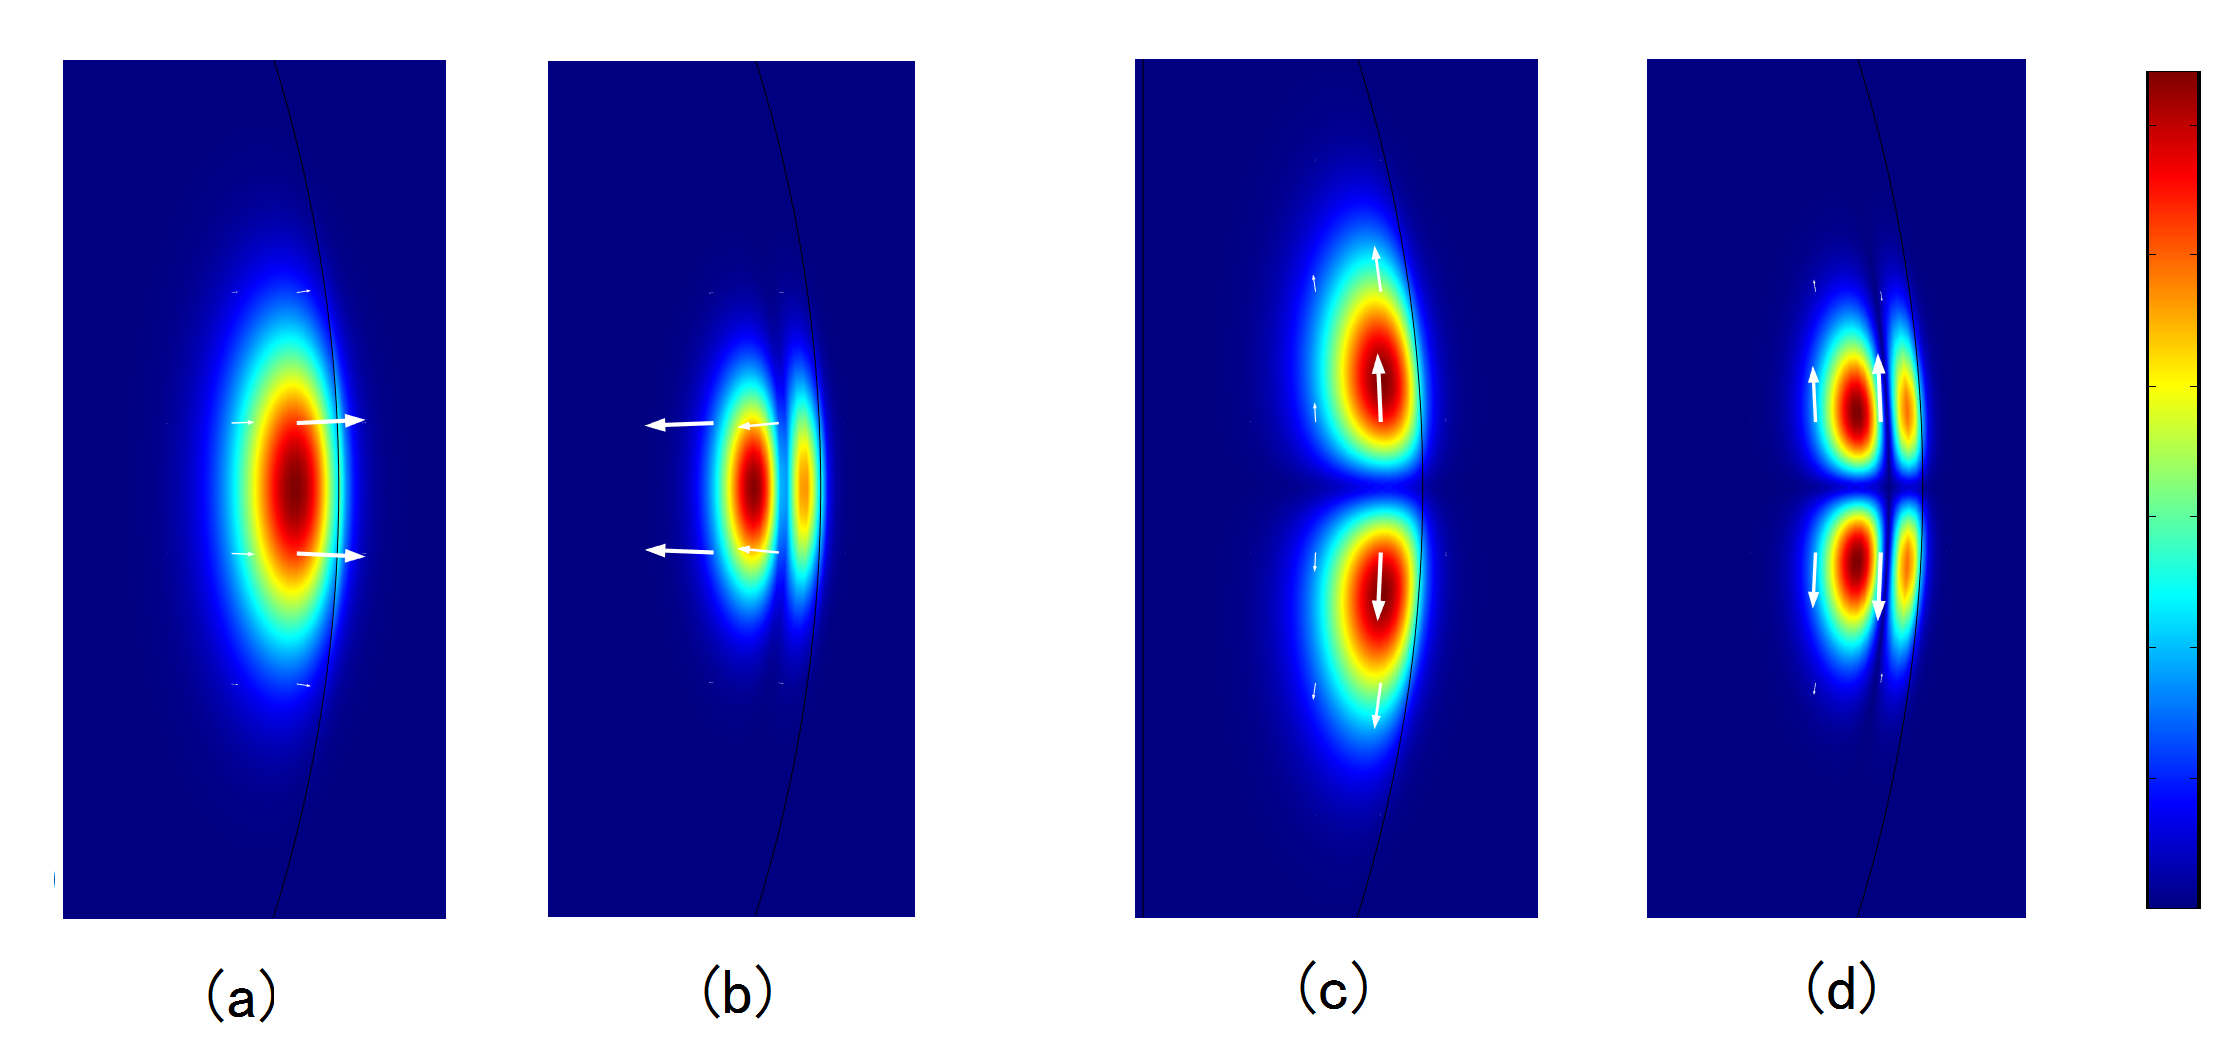
\includegraphics[width=14cm ]{TM1zoomwarrow_1_9319}
\caption{通过体二次非线性能够产生二次谐波的最低阶模式,电场强度切面分布仿真图。箭头为局部电场方向。a, 泵浦光TM基模,仿真波长1551.8nm。b, 二次谐波TM径向二阶角向基模$M=L, Q=2$,仿真波长775.96nm。c, 泵浦光TE角向二阶模$m=l-1, q=1$,仿真波长1549.2nm。d, 二次谐波TE径向二阶角向二阶模$M=L-1, Q=2$,仿真波长775.30nm。}
\label{pic:TM1zoomwarrow_1_9319}
\end{figure}

通过上述分析可知,TM模式在径向微分,且对模式没有附加要求,而TE模式在角向微分,且需要高阶模式。由图\ref{pic:TM1zoomwarrow_1_9319},由于模式在径向压缩得更严重,因而在同样归一化的条件下TM模式应当得到更大的微分值,且基模有利于达到更好的光纤锥耦合条件。为了定量说明这一点,使用式\ref{eq:gb}计算了直径62$\mu m$的微球腔中,如图\ref{pic:TM1zoomwarrow_1_9319}所示两组模式的二次谐波耦合系数,得到TM模式耦合系数的绝对值为TE模式耦合系数绝对值的18.62倍。

综合以上分析,虽然不同模式有所不同,但统计一个自由光谱范围中的全部模式,TM模式产生二次谐波的强度应当比TE模式要大,因此在实验上会观察到两个偏振产生二次谐波模式的数量和强度的统计特性不相同的情况。


\subsection{拉曼和二次合频信号}

%figures, a little bit about Raman

光子与二氧化硅中晶格振动产生的光学声子产生相互作用,会存在拉曼散射效应\cite{boyd2003nonlinear},产生一个波长更长的光子,拉曼光子的频率取决于材料本身的拉曼增益带。由于微腔对光场的增强作用,可以显著降低拉曼产生的阈值\cite{spillane2002ultralow, cai2000fiber, kippenberg2004ultralow}。 

在本次实验条件下,在某些模式中可以观察到拉曼信号,且在合适的条件下,拉曼光子与泵浦光子通过二次非线性效应进行合频,可以产生一个二次合频光子,进一步拓宽了可观测的频率范围。

\begin{figure}
\centering
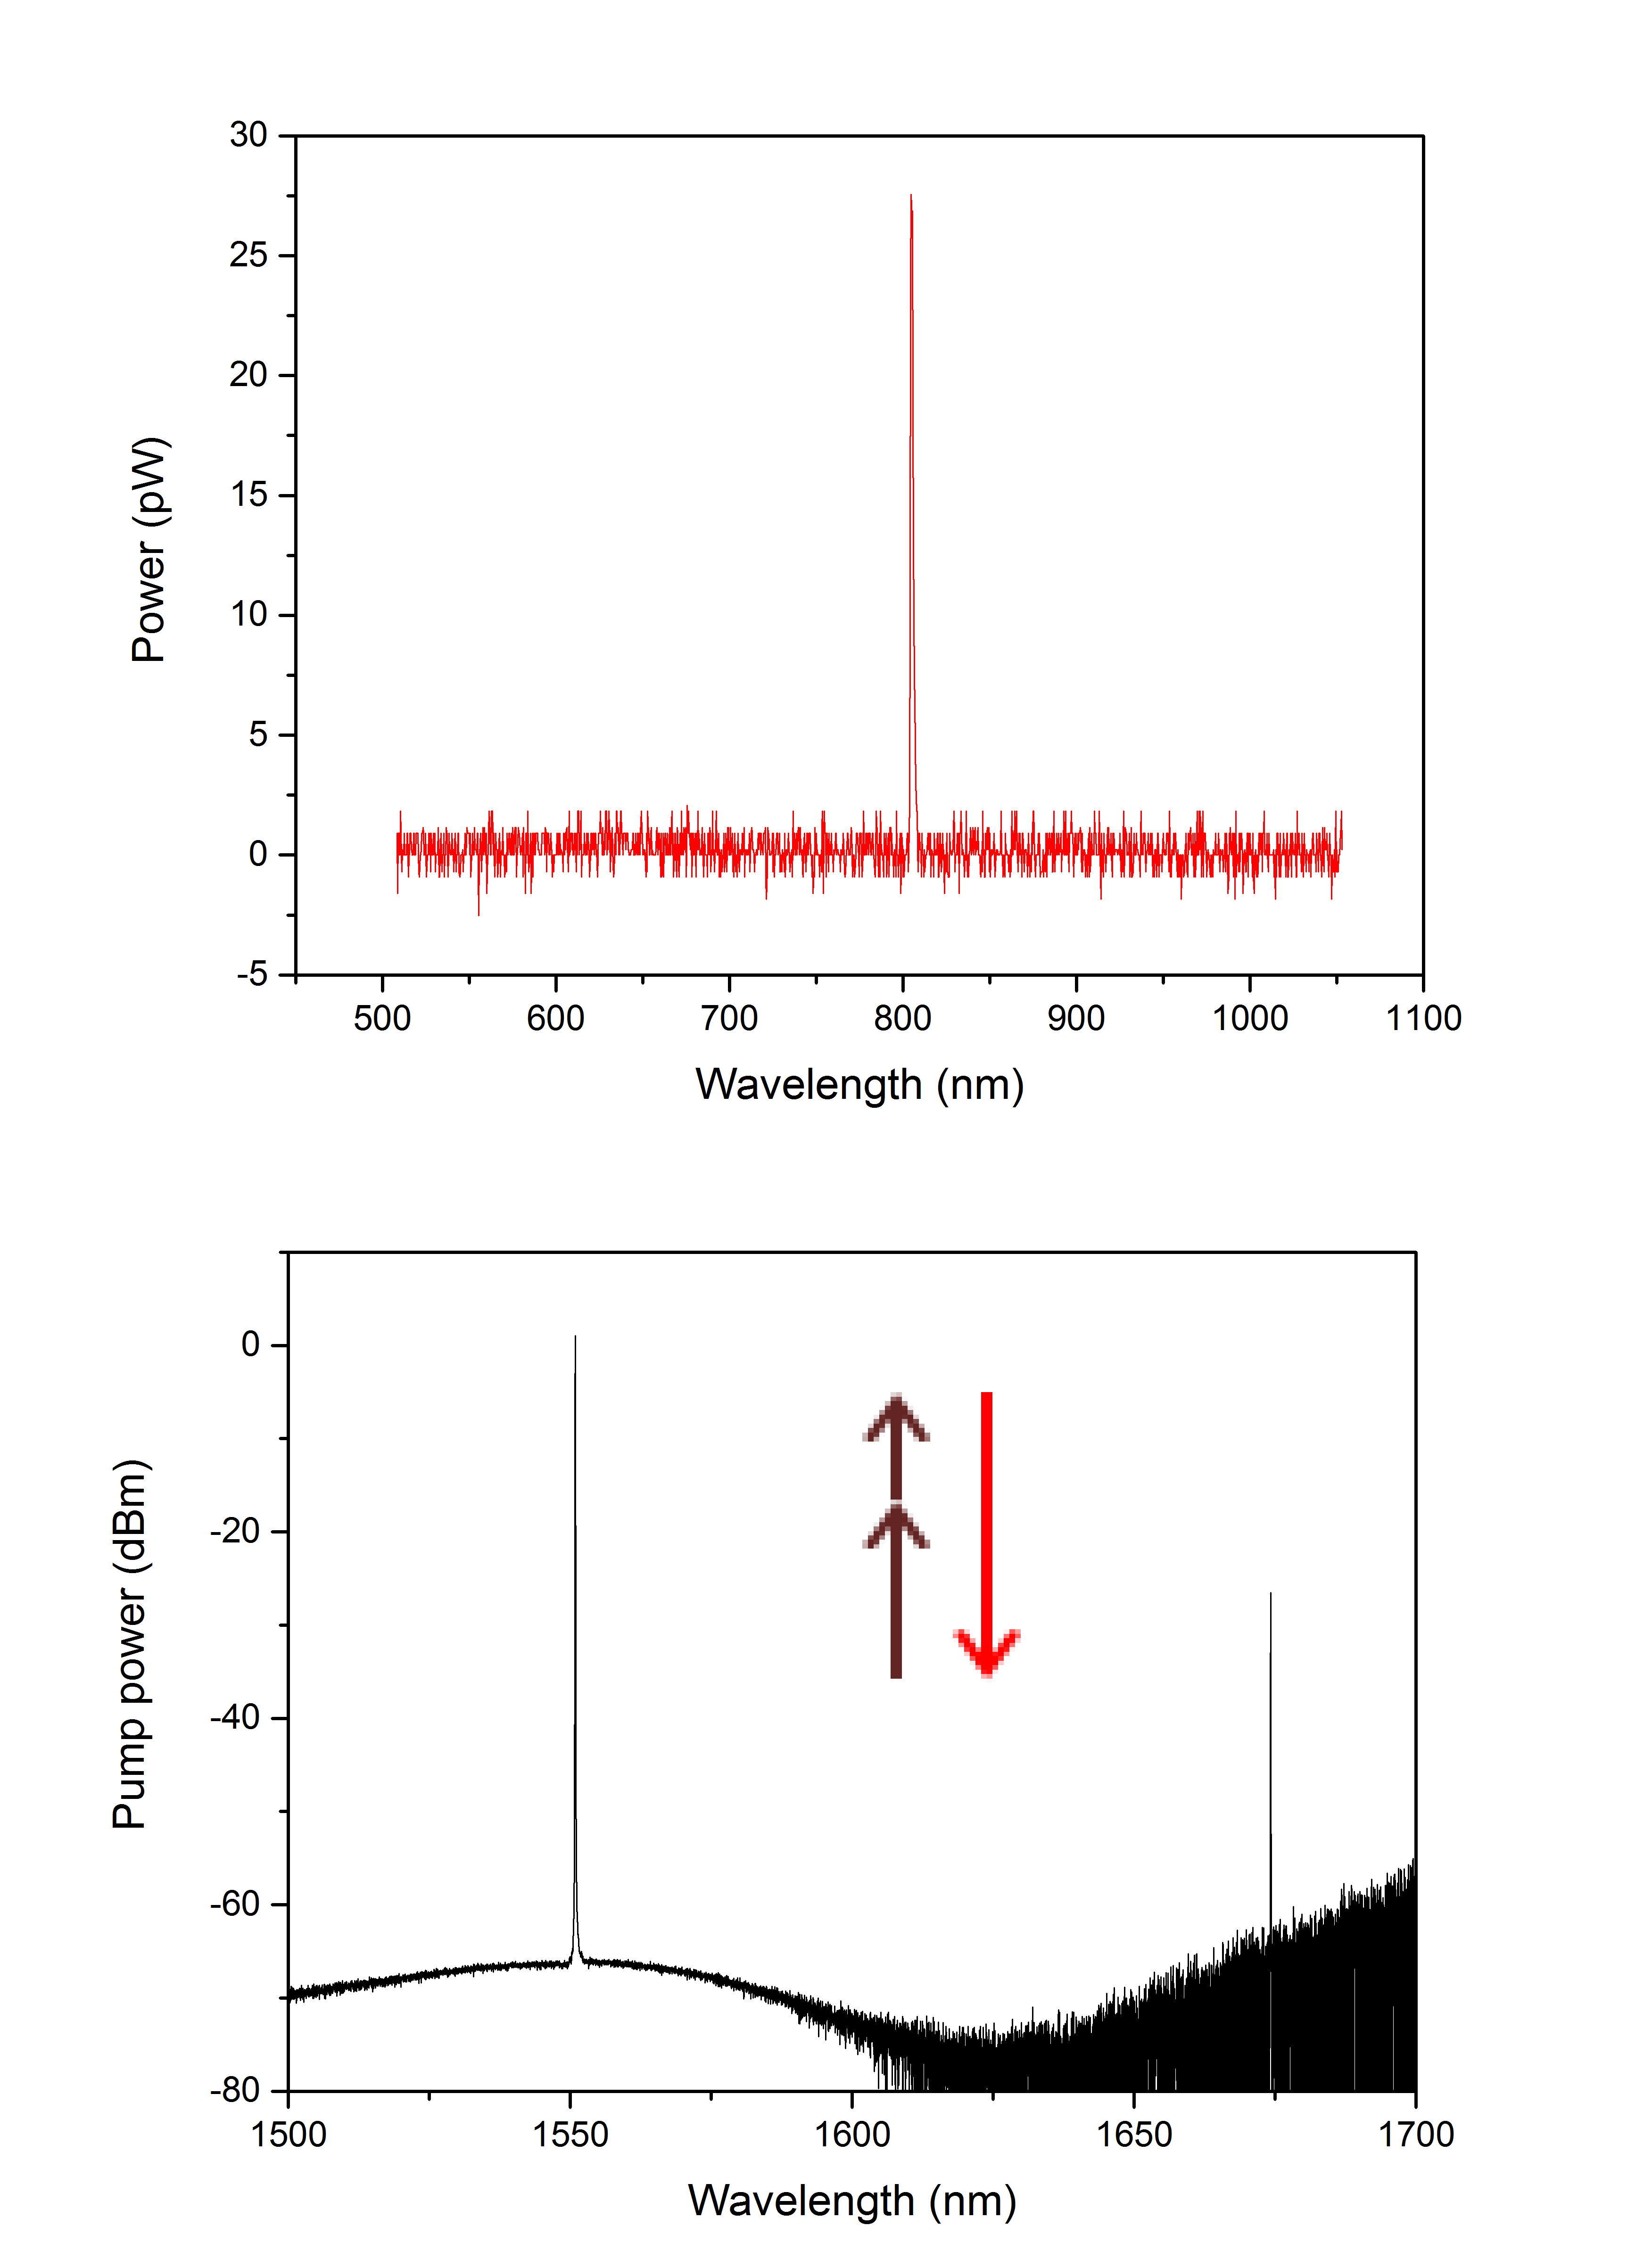
\includegraphics[width=14cm ]{FigRamanSF}
\caption{二次合频信号。a, 二次合频信号光谱图,波长为804.67nm。b,泵浦光波段光谱图,泵浦波长1550.88nm,拉曼光波长1674.22nm,插图为光子转换示意图。}
\label{pic:FigRamanSF}
\end{figure}

如图\ref{pic:FigRamanSF}所示为二次合频信号光谱图及其对应的泵浦波段光谱图,分析上图可以得出波长关系,$1/1550.88nm+1/1674.22nm = 1/804.63nm \approx 1/804.67nm$,满足二次合频关系。

\newpage
\section{结论}
\label{sec:conclu}

中心对称材料或非晶态材料的表面二次非线性已经在生物化学传感中得到了广泛的应用,而利用微型谐振腔对于光场的增强作用,可以极大地增强这种二次非线性。但就我们所知,几乎没有人对这些缺乏电偶极二次非线性的材料所制备的微腔进行深入的二次非线性研究。

因此,本文从理论和实验两方面入手。在理论上,首先探究了中心对称材料或非晶态材料中二次非线性的不同来源;接着探究了在微型谐振腔的框架中,这些二次非线性如何转化为基波和二次谐波之间的耦合系数;为了实际实验考虑,我们研究了有效产生二次谐波的前提,双共振条件,并提出了利用腔中显著的三次非线性效应(热效应和Kerr效应),来辅助调节腔模的位置,进而实现双共振条件;最后,我们分析了不同偏振在两种不同的非线性来源之下,产生二次谐波的效率。

实验上,设计了包含信号光光纤锥的实验装置,为能够有效收集二次谐波并观测其性质做好了铺垫;经过多次尝试,制备出了高品质因子,大小合适的微球腔,以及能够在两个波段同时达到临界耦合的双光纤锥,并探究出了灵活操纵双光纤锥的实验方法;在实验中证实了信号光光纤锥收集效率可以达到泵浦光光纤锥最优收集效率的13.73倍以上;探究了二次谐波信号功率随着泵浦光频率的变化关系,与理论中的近似洛仑兹线形有较好的对照;探究了二次谐波信号功率随泵浦光功率的变化关系,也与理论中的特征功率相对应;还给出了二次谐波产生功率和次数与偏振相对应的统计直方图,在实验上印证了理论中关于两种偏振二次非线性系数大小的相关结论;最后,在实验中还观测到了泵浦光和它对应的拉曼光子产生的二次合频光信号,拓宽了二次谐波波段的出射光谱范围。

本文填补了光学微腔非线性研究领域中的一大空白,拓宽了光学微腔出射光谱范围。非常重要的是,实验中在泵浦光功率882$\mu$W时(连续波激光器)就能够观测到功率约为0.4nW的二次谐波,而之前的实验中观测到二次谐波时,泵浦光功率高达209mW\cite{asano2016visible}。本实验展示了低功率二氧化硅微腔二次谐波产生的能力,为低功率生物化学分子的二次非线性方法传感作出了铺垫。同时,使用连续波激光器,与\cite{dominguez2011whispering}中使用脉冲激光器并将脉冲拉宽的实验方法相比,极大地简化了实验装置和操作。实验中的双光纤锥实验装置,作为良好的二次谐波收集系统,也可以应用在其他光学微腔弱信号探测和收集中。

由于双共振条件需要一定的腔内能量才能达到,而腔内能量又与输入光的频率密切相关,所以才得出类似于阶跃函数式的二次谐波功率-泵浦光功率依赖曲线,而非正规的二次曲线。为了得到二次曲线,应当有独立于泵浦光的腔内能量调控方式,并且有较好的腔内泵浦光能量衡量方法,这可以成为进一步实验的方向。

\section{致谢}

首先要感谢我的毕业设计导师刘玉玺教授,他在量子信息学引论这门课上为我打开了新方向的大门。虽然我加入组里的时间并不长,但刘老师从毕业设计选题,相关参考文献等各个方面对我给予了非常多的帮助和指导。不论是单独讨论还是组会上的工作讲解,刘老师的意见都让我受益匪浅。刘老师自由宽容的风格让我尤其印象深刻,学生有自己的想法,刘老师就会鼓励我们



\newpage
\bibliography{ref}
\end{document}




